% !TeX spellcheck = hu_HU
% !TeX encoding = UTF-8
% !TeX program = xelatex
% TODO Change language to en_GB (recommended) or en_US for English documents
\documentclass[11pt,a4paper,oneside]{report}             % Single-side
%\documentclass[11pt,a4paper,twoside,openright]{report}  % Duplex
\usepackage{xytree}
\usepackage{qtree}
\usepackage{multirow}
\newcommand{\edge}[3]{\texttt{#1}~$\xrightarrow#2$~\texttt{#3}}
\newcommand{\twoedges}[4]{\texttt{#1}~$\overset{#2}{\underset{#3}{\rightleftharpoons}}$~\texttt{#4}}
\newcommand{\bin}[3]{
    \texttt{#2}~$\xleftarrow1$~\texttt{#1}~$\xrightarrow2$~\texttt{#3}}
%\usepackage{tikz}

\input{include/packages}

%TODO Set the main variables
\newcommand{\vikszerzoVezeteknev}{Holló-Szabó}
\newcommand{\vikszerzoKeresztnev}{Ákos}

\newcommand{\vikkonzulensAMegszolitas}{}
\newcommand{\vikkonzulensAVezeteknev}{Ács}
\newcommand{\vikkonzulensAKeresztnev}{Evelin}

\newcommand{\vikkonzulensBMegszolitas}{}
\newcommand{\vikkonzulensBVezeteknev}{Nemeskey}
\newcommand{\vikkonzulensBKeresztnev}{Dávid}

\newcommand{\vikkonzulensCMegszolitas}{}
\newcommand{\vikkonzulensCVezeteknev}{}
\newcommand{\vikkonzulensCKeresztnev}{}

\newcommand{\vikcim}{Szemantikai elemzés gráf-transzformációkkal} % Cím
\newcommand{\viktanszek}{\bmemit} % Tanszék
\newcommand{\vikdoktipus}{\bsc} % Dokumentum típusa (\bsc vagy \msc)
\newcommand{\vikmunkatipusat}{szakdolgozatot} % a "hallgató nyilatkozat" részhez: szakdolgozatot vagy diplomatervet

\input{include/tdk-variables}
\newcommand{\szerzoMeta}{\vikszerzoVezeteknev{} \vikszerzoKeresztnev} % egy szerző esetén
%\newcommand{\szerzoMeta}{\vikszerzoVezeteknev{} \vikszerzoKeresztnev, \tdkszerzoB} % két szerző esetén

\newcommand{\todo}[1]{{\color{red}{TODO: #1}}}
\newcommand{\note}[1]{{\color{blue}{NOTE: #1}}}

%TODO Language configuration -- choose one
% Beállítások magyar nyelvű dolgozathoz
%\input{include/thesis-hu}
% Settings for English documents
\input{include/thesis-hu}

\input{include/preamble}

%--------------------------------------------------------------------------------------
% Table of contents and the main text
%--------------------------------------------------------------------------------------
\begin{document}

\pagenumbering{gobble}

%TODO These includes define guidelines -- remove these
%~~~~~~~~~~~~~~~~~~~~~~~~~~~~~~~~~~~~~~~~~~~~~~~~~~~~~~~~~~~~~~~~~~~~~~~~~~~~~~~~~~~~~~

\selectthesislanguage

%TODO Titlepage -- choose one from below
%~~~~~~~~~~~~~~~~~~~~~~~~~~~~~~~~~~~~~~~~~~~~~~~~~~~~~~~~~~~~~~~~~~~~~~~~~~~~~~~~~~~~~~
\include{include/titlepage}		   % Szakdolgozat/Diplomaterv címlap
%\include{include/titlepage-tdk}	% TDK címlap
%\include{include/titlepage-otdk}   % OTDK címlap


% Table of Contents
%~~~~~~~~~~~~~~~~~~~~~~~~~~~~~~~~~~~~~~~~~~~~~~~~~~~~~~~~~~~~~~~~~~~~~~~~~~~~~~~~~~~~~~
\tableofcontents\vfill


% Declaration and Abstract
%~~~~~~~~~~~~~~~~~~~~~~~~~~~~~~~~~~~~~~~~~~~~~~~~~~~~~~~~~~~~~~~~~~~~~~~~~~~~~~~~~~~~~~
\include{include/declaration} %TODO Hallgatói nyilatkozat -- TDK és OTDK esetén törlendő!
\pagenumbering{roman}
\setcounter{page}{1}

\selecthungarian

%----------------------------------------------------------------------------
% Abstract in Hungarian
%----------------------------------------------------------------------------
\chapter*{Kivonat}\addcontentsline{toc}{chapter}{Kivonat}

A Slime nyelv olyan nyelvek és nyelvtanok kiegészítésére való, melyek szintaxisa nagy mennyiségű redundáns kód írását teszi szükségessé. 
Nyelvi elemei a kiegészítendő nyelv vagy nyelvtan sablonjainak hatékony létrehozását, manipulációját és tárolását támogatják. 
A fordítót az ANTLR (ANother Tool for Language Recognition) segítségével valósítottuk meg. 
A Slime elsődlegesen IRTG (Interpreted Regular Tree Grammar) nyelvtanok tömör és átlátható leírására lett kifejlesztve. 
Az IRTG-t olyan nyelvtan fejlesztésére használjuk, amely két vagy több formalizmus (nyers szöveg, szintaktikai reprezentációk, szemantikai reprezentációk) közötti konverziót implementál gráftranszformációk segítségével. 
A Slime nyelvet IRTG nyelvtanok, ANTLR lexer nyelvtanok,  Android layout leíró XML kódok és HTML kódok előállítására használtuk. 
A legnagyobb nyereséget egy android layout esetében tapasztaltuk, ahol egy egyszerű gombos menü tömörítésére használtuk a Slime nyelvet: 30\%-kal lett kevesebb a sorok száma, de a kód nagy részét a sablonok előkészítése tette ki. Az előkészítést követően a gombokat már az addigi átlagosan tizenöt sor helyett három sorban lehetett megadni, ez sokkal több gomb esetén majdnem 80\%-os nyereséget jelent.
IRTG-k esetében az előkészítésen felül két sorra volt szükség az addigi hat sor helyett: egy sor az adatok definiálása, a másik pedig azok beszúrása a sablonba. Ez több IRTG szabály esetén akár 66\%-os nyereséget is jelenthet.
A program teljes forráskódja, szintaxisának és alapelemeinek leírása és számos példakód elérhető a \texttt{https://github.com/Hollo1996/SlimeAnUTLE} oldalon.

\vfill
\selectenglish


%----------------------------------------------------------------------------
% Abstract in English
%----------------------------------------------------------------------------
\chapter*{Abstract}\addcontentsline{toc}{chapter}{Abstract}

The Slime language is used for extending languages whose syntax requires the writing of highly redundant source code for certain applications. 
Its syntax supports efficient declaration, manipulation and storage of templates of the extended language. 
We implemented the compiler using ANTLR (ANother Tool for Language Recognition). 
The primary goal of developing Slime was a syntax that facilitates compact and clear formulation of IRTG (Interpreted Regular Tree Grammar) grammars. 
We use IRTGs to develop grammars which are capable of converting between two or more formalisms, such as raw text, syntactic, and semantic representations via graph transformations. 
Slime has been tested by implementing templates to generate IRTG grammars, ANTLR lexer grammars, Android layout XML and HTML sources.
Our Slime templates were most effective at generating Android layout code. Here we have managed to achieve a 30\% reduction in the lines of code needed
for implementing a menu. Most of the template content was initialization code, apart from which we only needed three lines of code per menu item as opposed to the avarage fifteen lines of code necessary in XML. This can result in even an 80\% reduction in necessary lines when implementing menus with a large number of items. In the case of generatating IRTG files, apart from the initialization code we only needed two lines of code per IRTG rule instead of the six in plain IRTG format. For an IRTG file with many rules this can mean a 66\% reduction in lines of code.
The source code of the language, the description of its syntax and its basic elements can be found at \texttt{https://github.com/Hollo1996/SlimeAnUTLE} alongside with several examples.

\vfill
\selectthesislanguage

\newcounter{romanPage}
\setcounter{romanPage}{\value{page}}
\stepcounter{romanPage}    %TODO Összefoglaló -- TDK és OTDK esetén nem kötelező


% The main part of the thesis
%~~~~~~~~~~~~~~~~~~~~~~~~~~~~~~~~~~~~~~~~~~~~~~~~~~~~~~~~~~~~~~~~~~~~~~~~~~~~~~~~~~~~~~
\pagenumbering{arabic}

%TODO import your own content
%----------------------------------------------------------------------------
\chapter{Bevezetés}
%----------------------------------------------------------------------------

Manapság egyre több technológia jelenik meg, aminek alapja az NLP (Natural Language Processing). Ezek a technológiák nagy része nem lenne megvalósítható szemantikai elemzés nélkül. A szemantikai elemzés célja, hogy egy nyers szövegből, vagy beszédhangból előállítsa annak a szemantikai reprezentációját. Ez a reprezentáció egy irányított gráf is lehet, amit ha a mondat szintaktikai szerkezetét reprezentáló fákból állítunk elő, akkor a teljes feladat felfogható egy gráf-transzformációként. 

Bár szemantikai elemzésre számos Deep Learning-es megoldás létezik, ezek pontatlansága nagy igényt teremt egy analitikus mély szemantikai elemzési módszerre. A gráf transzformációs megközelítés ígéretes eredményeket mutatott fel, mint például a Stanford Parser, ami TREGEX-ek segítségével végzi el tiszta analitikus módon a transzformációkat.
Több formalizmus is létezik a transzformációk leírására, mint például a HRG (hyperedge-replacement grammar) vagy az IRTG(interpreted regular tree grammars). Jelenleg is egy ezekkel kapcsolatos kutatás folyik az AUT tanszéken.

A kutatás során az ALTO(Algebraic Language Toolkit)-val dolgoztunk, ami a jelenlegi leghatékonyabb környezet IRTG-k futtatására. Ugyanakkor a kutatásnak állandó gátját jelenti, hogy az IRTG még egy fejletlen nyelvtan és nehezen átlátható; és az ALTO-ból is hiányoznak fontos funkcionalitások. A problémán sokat enyhítene, ha az IRTG szabályokat REGEX-ek segítségével is meglehetne hivatkozni.

Szakdolgozatom keretében egy templatelésre alkalmas nyelvet fejlesztettem ki, ami a Slime fantázianévre hallgat. Segítségével az IRTG nyelvtanokat tömörebben és átláthatóbban lehet definiálni. Mivel az ALTO java-ban készül, a nyelv Kotlinban készül ANTLRv4 segítségével. Még nincs teljesen kifejlődve, de a feladathoz szükséges megoldásokat tartalmazza. Ilyen például a template definiálás, egymásba ágyazás, regexxel hivatkozás és sok egyéb. Teljes formájában egy univerzális bővítmény lesz, ami bármely nyelv vagy szöveg felett használható.
 	 	 	
A dolgozat a következőképpen épül fel: 
\begin{itemize}
\item Az 2. fejezetben bemutatom a téma nyelvészeti vonatkozásait mutatom be, és a projektet, ami kapcsán készül.

\begin{itemize}
\item Az 1. alfejezetben mutatom be a szintaxis fogalmát, és annak bevett reprezentációit, avagy a szintaktikai fákat és az UD gráfokat.
\item A 2. alfejezetben mutatom be a szemantikai elemzés fogalmát, és a 4lang-ot.
Arra is kitérek, hogy mik a különbésgek az UD és a 4lang között.
\item A 3. alfejezetben a projekt célját mutatom be, ami kapcsán a szakdolgozat készül. 
\item A 4. alfejezetben mutatom be azt az eszközt, nyelvet és algebrákat, amivel dolgozunk a projekt során.
\item Az 5. alfejezetben mutatom be az eszköz és a nyelv hiányosságait, amik enyhítése a szakdolgozat termékének a célja.
\item Az 6. alfejezetben mutatom be a jelenlegi megoldásainkat a probléma orvoslására.
\end{itemize} 

\item Az 3. fejezetben mutatom be magát a nyelvet.

\begin{itemize}
\item Az 1. alfejezetben mutatom be a szakdoga termékét jelentő nyelvet, a Slime-ot.
\item A 2. alfejezetben ismertetem a tervezés szempontjait, amiken a design döntések többsége nyugszik.
\item A 3. alfejezetben ismertetek más megoldásokat a problémára, amik a nyelv megszerkesztéséhez is alapul szolgáltak.
\item A 4. alfejezetben mutatom be magának a Slime-nak a részletes működését és szintaxisát.
\item Az 5. alfejezetben ismertetem az implementáció mögötti technológiákat és megoldásokat nagy vonalakban.
\item Az 6. alfejezetben mutatom be a nyelv fejlesztésének eddigi és ez utáni ütemtervét.
Az ambíciók demonstrációjának céljával betekintést nyújtok minden tervben lévő funkcionalitásra.
\item Az 7. alfejezetben példákkal szolgálok a Slime felhasználására több alárendelt nyelvvel is.
\end{itemize}

\end{itemize} 

%----------------------------------------------------------------------------
\chapter{Szemantikai elemzés gráf-transzformációkkal}
\label{sec:spwgt}
%----------------------------------------------------------------------------
\section{Szintaxis}
\label{sec:syntax}
%----------------------------------------------------------------------------
Azon szabályok összességét hívjuk szintaxisnak, amelyek mentén a szavakból szószerkezeteket és mondatokat építhetünk. Ide tartoznak például a szavak sorrendjére vonatkozó megkötések. A nyelvészetben a mondatrészek közötti viszonyokat többféle módon lehet szemléltetni, ebben a fejezetben két ilyen formalizmust ismertetek röviden.

%----------------------------------------------------------------------------
\subsection{A közvetlen összetevős elemzés}
\label{sec:tree}
%----------------------------------------------------------------------------

A természetes nyelvek struktúráját számos nyelvészeti elméleti keretben \texttt{környezetfüggetlen nyelvtan} segítségével írják le.

Környezetfüggetlen nyelvtannak egy $G=(V,\Sigma ,P,S)$ rendezett négyest nevezünk, ahol:

\begin{itemize}
	\item \emph{$V$} s változók halmaza, avagy a nem terminális abc.
	\item \emph{$\Sigma$} terminális ábécé amire $ V \cap \Sigma =\varnothing $
	\item \emph{$S \in N$} a kezdőszimbólum
	\item \emph{$P$} egy véges halmaz, az ún. levezetési vagy produkciós szabályok halmaza. P elemei
$\alpha \to \beta$ alakúak, $\alpha$ és $\beta$ tetszőleges, V és $\Sigma$ elemeiből képzett sorozat, az egyetlen
megkötés, hogy $\alpha$ tartalmazzon legalább egy változót is ($\beta$ lehet akár az üres szó is).
\end{itemize}
\cite{Friedl:2003}
Ebben a nyelvtanban a terminális szimbólumok a szavak, a nemterminális szimbólumok pedig a \textit{szófaji kategóriák}, \textit{frázisok} és \textit{mondatok}. A szófaji kategóriák (pl. \textit{főnév}, \textit{ige}) azok a szimbólumok, amik közvetlen szavakká írhatóak át, mindegyik pontosan egy szóvá. Frázisoknak azokat a szerkezeteket nevezzük, amelyeknek egy-egy szó a feje, és az adott szó szófajáról nevezzük el (pl. \textit{NP - noun phrase, főnévi frázis/kifejezés}). Ezeket szófaji kategóriák és más frázisok sorozatává írhatjuk át, a mondatokat pedig frázisokká.
A lehetséges levezetési fákon kivehető az egyes nemterminális szimbólumtípusok rétegződése, hierarchiája.  A~\ref{fig:john_zarojel} ábrán láthatjuk a \textit{John loves Mary.} mondat szerkezetére vonatkozó újraíró szabályokat.

\begin{figure}[h]
\texttt{S( NP( NNP( John ) ), VP( VBZ( loves ),  NP( NNP( Mary ) ) ) ) )} :
\begin{itemize}
\item$S \to NP, VP$ 
\item$NP \to NNP$
\item$VP \to VBZ, NP$
\item$NNP \to John | Mary$
\item$VBZ \to loves$
\end{itemize}
\caption{A \textit{John loves Mary.} mondat újraíró szabályai}
\label{fig:john_zarojel}
\end{figure}

A zárójelezés és az ágrajz egymással ekvivalens ábrázolási módok. A fenti mondat ágrajzát a~\ref{fig:john_agrajz} mutatja.

\begin{figure}[h]
\centering
\graphicspath{./}
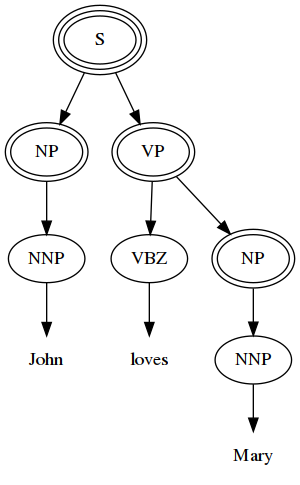
\includegraphics[scale=0.32]{figures/dots/john_agrajz.png}
\caption{A \textit{John loves Mary.} mondat ágrajzon ábrázolva}
\label{fig:john_agrajz}
\end{figure}

A fa levelei a szavak(\textit{John}, \textit{loves}, \textit{Mary}), amik fölött a szófaji kategóriák (\textit{NNP}, \textit{VBZ}) helyezkednek el, mint unáris csúcsok.
Az \textit{NP}, \textit{VP} a főnévi és igei kifejezéseket jelölik, az \textit{S} pedig a mondat gyökere (az angol \textit{sentence} szó után).


%----------------------------------------------------------------------------
\subsection{Dependenciaelemzés és az UD}
\label{sec:ud}
%----------------------------------------------------------------------------
A dependencia-alapú megközelítés szerint a szintaktikai szerkezet lexikai elemekből áll, amelyeket bináris kapcsolatok kötnek össze. A \texttt{dependencia} fogalma azt jelenti, hogy a szavak (\texttt{fej} és \texttt{dependens}) irányított kapcsolatokkal vannak összekötve.  Általában az állítmány a gráf gyökércsomópontja vagy a strukturális középpontja a mondatnak. A különböző elméleti keretekben közös vonás, hogy a mondat szerkezetét a fejek és dependensek közötti viszonyok adják, összefoglalásért lásd \cite{Nivre:2005}.

A dependencianyelvtanok az információt egy DAO gráfon szemléltetik, amelyek csúcsai a szavak, és élei pedig a szavak közötti viszonyok. Az ilyen függőségi gráfok leírására többféle formalizmus létezik. Mi a kutatásunk során az \texttt{UD}-t (Universal Dependencies)\cite{deMarneffe:2014} használtuk.

Az UD projekt\footnote{\url{http://universaldependencies.org/}} egy nyelvek közötti konzisztens annotációs rendszer és fa-adatbázis hatvannál is több nyelvre. Kategóriák és annotációk univerzális készletét nyújtja, miközben megenged nyelvfüggő kiterjesztéseket is. Az UD a Stanford Dependencies-ből \cite{deMarneffe:2008} fejlődött ki, és lehetővé teszi nyelvfüggetlen dependenciaparszerek kiértékelését.

\begin{figure}[h]
\centering 
\xytext{
    \xybarnode{I} 
    &~~~&
    \xybarnode{saw} 
      \xybarconnect(UL,U){-2}"_{\small nsubj}"
      \xybarconnect[18](U,UR){8}"^{\small punct}"
      \xybarconnect[12](UR,UR){6}"^{\small obj}"
    &~~~&
    \xybarnode{the} 
    &~~~&
    \xybarnode{white} 
    &~~~&
    \xybarnode{cat} 
      \xybarconnect[8](U,U){-4}"_{\small det}"
      \xybarconnect(UL,U){-2}"_{\small amod}"
    &~~~&
    \xybarnode{.}
}
\caption{Az \textit{I saw the white cat.} mondat függőségi elemzése}
\label{fig:deptreeEN}  
\end{figure}

\begin{figure}[h]
\centering 
\xytext{
    \xybarnode{A} 
    &~~~&
    \xybarnode{fehér} 
    &~~~&
    \xybarnode{macskát} 
      \xybarconnect[8](U,U){-4}"_{\small det}"
      \xybarconnect (UL,U){-2}"_{\small amod}"
    &~~~&
    \xybarnode{láttam} 
      \xybarconnect(U,UR){-2}"_{\small obj}"
      \xybarconnect(UR,UL){2}"^{\small punct}"
    &~~~&
    \xybarnode{.}
}
\caption{Az \textit{A fehér macskát láttam.} mondat függőségi elemzése}
\label{fig:deptreeHU}  
\end{figure}

A~\ref{fig:deptreeEN} és~\ref{fig:deptreeHU} ábrákon jól látszik az UD nyelvfüggetlensége. A mondat angol és magyar verziójában a szavakat megfeleltetve az élek is könnyen megfeleltethetőek.
Itt az élek jelentése a következő:
\begin{itemize}
\item \emph{punct : } 
A feje az állítmány, a dependense pedig a mondatot záró pont vagy más írásjel.
\item \emph{det : } 
A szerkezet fejét a rá vonatkozó névelővel (determinánssal) köti össze. 
Például a \textit{The} a \textit{cat}-nek, és az \textit{a} pedig a \textit{macskát}-nak determinánsa.
\item \emph{amod: } 
Azt jelöli, hogy a fejnek a dependens a mellékknévi módosítója.
Például a \textit{white} a \textit{cat}-et, a \textit{fehér} a \textit{macskát} szót módosítja.
\item \emph{obj : }  
A feje az állítmány, a dependense pedig a tárgy.
Jelen esetben a \textit{cat} vagy a \textit{macskát} a mondat tárgya.
\item \emph{nsubj : } 
Azt jelöli, hogy a fejnek a dependens a névszói alanya. 
Ez azért nem jelenik meg a magyar mondat esetén, mert a magyarban nem vagyunk kötelesek megadni az "én" személyes névmást, mivel az állítmány ragozása jelöli a rejtett alanyt.
\end{itemize}

%----------------------------------------------------------------------------
\section{Szemantika}
\label{sec:semantics}
%----------------------------------------------------------------------------

A szemantika a nyelvészet jelentéssel foglalkozó részterülete. A \texttt{szemantikai elemzés} (semantic parsing) célja, hogy a nyers szövegből, vagy valamely szintaktikai reprezentációból előállítsa a szemantikai reprezentációkat.

A legmodernebb, jellemzően mélytanulás-alapú rendszerek szóvektorokat alkalmaznak: a szavak jelentését sokdimenziós terek vektoraiként reprezentálják. Ezekkel a módszerekkel a legnagyobb probléma az, hogy csak nagyon csekély belátást biztosítanak a háttérben meghúzódó struktúrákra.

Ezzel ellentétben mi a kutatás során fogalmi hálózatokon alapuló szemantikai reprezentációkat alkalmaztunk, amelyek lehetővé teszik a struktúrák explicitebb analízisét, így jobb rálátást nyújtanak olyan problémákra, mint a természetes nyelvi következtetés (natural language inference) vagy a gépi szövegértés (machine comprehension).

%----------------------------------------------------------------------------
\subsection{4lang}
\label{sec:4lang}
%----------------------------------------------------------------------------
A \texttt{4lang}  \cite{Kornai:2015} egy formalizmus, ami irányított gráfokat épít szemantikai reprezentáció céljával. A gráfban a csúcsok nem szavakat, hanem nyelvfüggetlen fogalmakat jelölnek. Ezeknek a fogalmaknak már nincsenek nyelvtani jellemzőik és a kompetens beszélők közös tudását reprezentálják a fogalomról. Például a \textit{fagy} mint főnév vagy mint ige, illetve a \textit{fagyás} vagy \textit{fagyott} szavak nincsenek megkülönböztetve a 4lang reprezentációban \cite{Recski:2018}. Ezáltal a 4lang fogalmak és a nekik egy nyelvben megfelelő szavak között egy-a-többhöz kapcsolat áll fenn.

A csúcsokat háromféle él kapcsolhatja össze:
0-él reprezentálja a tulajdonságokat. Például \edge{virág}{0}{szép}, az \textit{$IS\_A$} viszony \edge{virág}{0}{növény} és unáris predikáció \edge{virág}{0}{bimbózás}.
Az 1 és 2-élek bináris predikációkat kapcsolnak az argumentumaikhoz, például \bin{szeretet}{James}{kutya}.

Létezik egy másik élkonfiguráció is, ami megjelenhet 4lang gráfban, \twoedges{$w_1$}{1}{0}{$w_2$} . Erre azért van szükség, hogy konzisztensen lehessen jelölni a tárgy és predikátum közötti viszonyt. Vegyük például a \textit{I am writing} (\textit{Én éppen írok})  mondatot az \edge{i}{0}{write} 4lang gráffal és az \textit{I am writing a letter} (\textit{Én egy levelet írok éppen}) mondatot az \bin{write}{i}{letter} gráffal . Ez a két példa a dupla él nélkül azt jelentené, hogy  az \textit{I} és a \textit{write} között attól függ a viszony, hogy adott-e a tárgy vagy sem. \cite{Recski:2018}

A 4lang könyvtár tartalmaz eszközöket, amelyek képesek 4lang gráfokat építeni nyers szövegből és szótári definíciókból (text\_to\_4lang, dict\_to\_4lang). A dep\_to\_4lang 4lang viszonyokat nyer ki szövegből a Stanford Parser \cite{deMarneffe:2008} kimenetének a feldolgozásával és a Stanford függőségek 4lang részgráfokká való leképezésével.
4lang a neve egy kézzel alkotott  fogalmi szótárnak is, amely négy nyelven (magyar, angol, latin, lengyel) tartalmazza több mint 2000 fogalom nyelvfüggetlen definícióját. \cite{Kornai:2013}


%----------------------------------------------------------------------------
\subsection{A 4lang és az UD különbségei}
\label{sec:4LvsUD}
%----------------------------------------------------------------------------
A munkánk során, mint majd alaposabban is bemutatom a nyelvtan generálásánál, alaposan kihasználtuk a 4lang és az UD közötti hasonlóságot. Mindkét esetben irányított gráfokról beszélünk: a csúcsok megfeleltethetőek a szavaknak, és az élek a szavak közötti viszonyokat jelölik, ezek a viszonyok sok esetben megfeleltethetőek egymásnak: például az \texttt{amod} dependencia leképezhető a \edge{$w_1$}{0}{$w_2$} 4lang-éltípusra.

A kettő között ugyanakkor fontos elméleti és jelölésbeli különbségek vannak. Az UD a mondatok szintaxisát reprezentálja, míg a 4lang a szemantikáját (jelentését). Az UD-ben a csúcsok maguk a szavak, míg a 4lang-ban a szavaknak megfeleltethető fogalmak. Az UD élei a szavak közötti nyelvtani viszonyt jelölik, a 4lang élek pedig a szavak közötti szemantikai kapcsolatokat. A 4lang élek és az UD függőségek között egy a többhöz viszony áll fenn, ahogy a szavak és a 4lang-beli fogalmak között is. Ez azt jelenti, hogy az UD közvetetten tartalmazza a szemantikára vonatkozó információkat is.

    \begin{table}
      \centering
      \begin{tabular}{ll}
      \textbf{UD dependencia} & \textbf{4lang él}                 \\ \hline
      advcl               & \edge{$w_1$}{0}{$w_2$}        \\
      advmod              &                               \\
      amod                &                               \\
      nmod                &                               \\
      nummod              &                               \\ \hline
      appos               & \twoedges{$w_1$}{0}{0}{$w_2$} \\
      dislocated          &                               \\ \hline
      csubj               & \twoedges{$w_1$}{1}{0}{$w_2$} \\
      nsubj               &                               \\ \hline
      ccomp               & \edge{$w_1$}{2}{$w_2$}        \\
      obj                 &                               \\
      xcomp               &                               \\ \hline
  
      \multicolumn{2}{l}{\textbf{A \texttt{case} kezelése}}      \\ \hline
      case + nmod         & $w_1\xleftarrow1$ $w_3$ $\xrightarrow2w_2$ \\
      case + nsubj        &                                            \\
      case + obl          &                                            \\ \hline
  
      \multicolumn{2}{l}{\textbf{Angol nyelvspecifikus altípusok}}                           \\ \hline
      obl:npmod           & \edge{$w_1$}{0}{$w_2$}                            \\ \hline
      nmod:tmod           & $w_1\xleftarrow1$ \texttt{AT} $\xrightarrow2w_2$  \\
      obl:tmod            &                                                   \\ \hline
      nmod:poss           & $w_2\xleftarrow1$ \texttt{HAS} $\xrightarrow2w_1$
      \end{tabular}
      \caption{UD dependenciák leképezése 4lang részgráfokra (\cite{Acs:2019}, \cite{Recski:2018} alapján).}
      \label{table:deps}
      \end{table}

Bár a mondat UD gráfjából a 4lang gráfja levezethető, a két formalizmus tartalma mégsem ekvivalens. A 4lang gráfból már nem mindig vezethető le egyértelműen az UD.

\begin{figure}[h]
\centering 
\xytext{
    \xybarnode{The} 
    &~~~&
    \xybarnode{white} 
    &~~~&
    \xybarnode{cats} 
      \xybarconnect[8](U,U){-4}"_{\small det}"
      \xybarconnect (UL,U){-2}"_{\small amod}"
}


\xytext{
    \xybarnode{white} 
    &~~~&
    \xybarnode{cat} 
      \xybarconnect (UL,U){-2}"_{\small 0}"
}
\caption{A 'The white cat' UD és 4lang gráfja }
\label{fig:thewhitecat}  
\end{figure}

A~\ref{fig:thewhitecat}. ábra szemlélteti, hogy az \textit{amod} él megfeleltethető egy \textit{0} élnek. Az is megfigyelhető, hogy a névelő nem jelenik meg a 4lang gráfban. A \textit{cats} is elveszti a többes számát, mivel fogalommá általánosul, így a 4lang gráf nem is alakítható vissza egyértelműen UD gráffá ez elveszett információk miatt.


%----------------------------------------------------------------------------
\section{A kutatás célja}
\label{sec:goals}
%----------------------------------------------------------------------------

A kutatásunk célja az, hogy a nyers szöveg és a fent leírt interpretációk bármelyikéből le tudjuk a többit generálni. Ha az egyik interpretációhoz a másikból több is tartozik, akkor képesek akarunk lenni az összes verziót legenerálni és a legalkalmasabbat automatikusan kiválasztani valószínűségi súlyozás segítségével. Minél kevesebb nyelvet szeretnénk használni, és minél kevesebb módszertant. Ez utóbbi szemponttól azt várjuk, hogy könnyebb lesz a kódot karbantartani és bővíteni további interpretációkkal. Mindezt hatékonyan is szeretnénk csinálni. E téren az alap célunk egy négyzetes lefutási idő a bemenet méretének függvényében. Ezeknek a megkötéseknek az IRTG eleget tesz, hiszen nagyon eltérő interpretációk esetében is legfeljebb interpretációk száma plusz egy nyelvet kell használnunk. Ugyanakkor, ha kiegészítjük az IRTG-t egy összetettebb gráfalgebrával, az képes lehet minden interpretáció hatékony leírására és mindehhez két nyelvet kellene használnia.

%----------------------------------------------------------------------------
\section{Az IRTG és az alárendelt algebrák}
\label{sec:aists}
%----------------------------------------------------------------------------
Ebben a fejezetben a kutatás során használt környezetről (Alto), formalizmusról (IRTG), algebrákról(SA, TTA, SGA), hátrányaikról és az ezeket kiküszöbölő ideiglenes megoldásainkról lesz szó.

%----------------------------------------------------------------------------
\subsection{Az Alto}
\label{sec:Alto}
%----------------------------------------------------------------------------
A kutatás során a kódot az Alto-val\footnote{\url{https://github.com/coli-saar/Alto}} (Algebraic Language Toolkit) fordítjuk és futtatjuk. Az Alto egy nyílt forrású parszer, többféle algebrát is megvalósít, amelyek IRTG-be ágyazva használhatók, mint például az \texttt{s-graph} és a \texttt{tag tree} algebrák. Ezen kívül is szabadon bővíthető új algebrákkal. Már korábban is használták gráftranszformációra és szemantikai elemzésre is, lásd \cite{Koller:2015}, \cite{Groschwitz:2015}. Nagy előnyt jelent, hogy Java-ban lett implementálva, így szinte bármely platformon futtatható. Rendelkezik grafikus és konzolos felhasználói felülettel is.


%----------------------------------------------------------------------------
\subsection{Az IRTG}
\label{sec:irtg}
%----------------------------------------------------------------------------
Az IRTG (Interpreted Regular Tree Grammar, interpretált reguláris fa-nyelvtan) \cite{Koller:2011} egy kontextusfüggetlen nyelvtan, ami egy vagy több algebrába beágyazott újraíró szabályokból áll.

\begin{figure}[h]
\begin{verbatim}
NP -> _NP2_amod_JJ_NN(JJ, NN)
[string] *(?1,?2)
[tree] NP2(?1, ?2)
[ud] merge(f_dep(merge("(r<root> :amod (d<dep>))", r_dep(?1))),?2)
[fourlang] merge(f_dep(merge("(r<root> :0 (d<dep>))", r_dep(?1))),?2)
\end{verbatim}
\caption{Egy, az \texttt{amod} relációt leíró IRTG-szabály négy algebrával}
\label{fig:amod_irtg}
\end{figure}

A szabálysorok egy környezetfüggetlen nyelvtan átírási szabályait adják meg. A szabályok feldolgozásakor először egy \texttt{levezetési fa} (derivation tree) épül, amelyek a nonterminálisokat lecserélő szabályokat tartalmazzák. Egy szabályt a következő módon lehet definiálni (a sablonban a változó részeket \{\$ \$\} zárójellel jelöltem, ahol a \$ a Slot kifejezésből ered, a \{\} pedig a nem szöveg elemeket jelöli):
\begin{verbatim}
[{$ interpretáció neve $}] {$ interpretáció lépése $}
\end{verbatim}
A interpretációk nyelve és kimenete többféle is lehet.  Választható például a szöveg kimenetű \texttt{string algebra}, a csúcssorrendet tartó, fa kimenetű \texttt{tag tree algebra}, vagy  az irányított gráf kimenetű \texttt{s-graph algebra}. Az algebrák és az interpretációk között egy a többhöz kapcsolat van. Az interpretációk egymástól teljesen függetlenek. Egy szabályban minden interpretációt meg kell adni. Minden átírás során, minden interpretációra vonatkozó derivációba beszúródnak az alkalmazott szabályban az interpretációhoz tartozó lépések. A beszúrás helyét ?{\$ szám \$}-ként jelölik minden interpretációban. Itt a szám annak a jobb oldali nemterminálisnak a sorszáma, amely átírása során szúródik be az alkalmazott átírási szabálynak az interpretációhoz tartozó lépése. Az IRTG futtatásakor bármelyik interpretáció lehet a bemenet. Az Alto a bemeneti interpretáció algebrájának megfelelő formátumú bemenetet vár. A futás során az Alto keres a bemenethez egy olyan levezetést, ami megfelel a környezetfüggetlen nyelvtannak és a bemenetet adja eredményül. Ezt követően a levezetési fa szerint felépíti a többi interpretációt is, és végrehajtva őket, előállítja a kimeneteket.

Tekintsük az 1.ábrán bemutatott szabályt. Ez a szabály egy melléknévből (adjective, JJ) és egy főnévből (noun, NN) készít egy két gyermekű főnévi kifejezést (noun phrase, NP). A két szó között melléknévi módosítói (adjectival modifier, amod) viszony áll fenn az UD gráfban. Ennek megfelelően neveztük el a szabályt \texttt{\_NP2\_amod\_JJ\_NN}-nek. Az interpretációk sorban a nyers szöveg, a szintaktikai fa, az UD gráf és a 4lang gráf.
Itt minden reprezentációban a \texttt{?1} és \texttt{?2} az, ahova a \texttt{JJ} és \texttt{NN} jobb oldali nemterminális szimbólumok átírásánál keletkező kifejezések kerülnek. Ezek az interpretációk bemenetei. Jelen esetben a \texttt{?1} a \texttt{JJ} és a \texttt{?2} az \texttt{NN} szimbólum interpretációinak a helye. A két jobb oldali nemterminális kiértékelése után minden interpretációba a vele azonos interpretáció kimenete kerül, stringé a stringbe stb.

A string interpretációhoz a string algebra tartozik. Jelen esetben a bemeneti két szót fűzi össze. A tree interpretációhoz a tag tree algebra tartozik, ami egy \texttt{NP2} címkéjű csúcs alá szúrja be a két bemenetet. Ez az algebra állítja elő a szintaktikai fát. A bemenete két-két csúcs.  A negyedik és ötödik sorhoz is az s-graph algebra tartozik. Mindkettő irányított éllel köti össze a két bemenetet. Az UD egy \texttt{amod}, a 4lang pedig egy \texttt{0} címkéjű éllel. Itt mindkét esetben mindkét bemenet csak egy címkézett csúcs. A nevüknek megfelelő gráfokat állítják elő. Magasabb szintű szabályoknál már az UD és 4lang bemenetek összetett irányított gráfok lesznek. Mi elsősorban az előbb említett három algebrát használjuk, de ezeken kívül más algebra is használható az IRTG nyelvben, mint például a \texttt{wide string algebra}, a \texttt{tree with arities algebra} vagy a \texttt{set algebra}\footnote{\url{https://bitbucket.org/tclup/alto/wiki/Algebras}}. Ezek nem részei a dolgozat fókuszának.



%----------------------------------------------------------------------------
\subsection{A string algebra}
\label{sec:sa}
%----------------------------------------------------------------------------
Az SA (\texttt{string algebra} az összes IRTG alatt elérhető algebra közül a legegyszerűbb. Itt csak szövegek konkatenációjára (összefűzésére) van lehetőség. A bemenet és kimenet nem tartalmaz slotokat vagy egyéb nyelvi elemeket. A műveletet a következő formátumban lehet megadni:
\begin{verbatim}
*( {$ szöveg1 $}, {$ szöveg2 $} )
\end{verbatim}

Egymásba is ágyazható több konkatenáció:
\begin{verbatim}
*( {$ szöveg1 $}, *( {$ szöveg2 $}, {$ szöveg3 $} ) )
\end{verbatim}

Például a \textit{*( "Every mouse”, *( “loves”, “cheese.” ) )} kifejezés az \textit{Every mouse loves cheese.} szöveget adja vissza. Ez a konkatenáció kommutatív és asszociatív.


%----------------------------------------------------------------------------
\subsection{A tag tree algebra}
\label{sec:tta}
%----------------------------------------------------------------------------
A TTA (\texttt{tag tree algebra})-nak, mint az SA-nak, csak egy művelete van, a \textit{merge} (egyesítés). A TTA esetében viszont  már a bemenetek nem nyers szövegek, hanem csúcs sorrend tartó fa gráfok. Tartalmazhatnak slot-okat, amiket TTA esetében \textit{hole}-nak(lyuk) nevezünk. A hole-okat ‘*’-gal jelöljük. Nem lehet őket címkékkel vagy más módon megkülönböztetni, sem eltörölni. A gráf csúcsaiba helyezhetőek. Az ilyen slot-okat tartalmazó fákat nevezzük \textit{tag tree}-nek. A TTA merge műveletének két operandusa van. Mindkét operandus egy tag tree. A jobb oldali fát szúrjuk be a bal oldali fa minden hole-jába a merge során. A merge jele a ‘@’ szimbólum, és se nem kommutatív, se nem asszociatív. A fákat zárójelekkel adjuk meg. Egy csúcs közvetlen gyermekeit és az azok alatti részfát a tőle jobb oldali zárójelben kell megadni vesszőkkel elválasztva. Például így írható le a \textit{John loves Mary} mondat szintaktikai fája:

S3( NP1( NNP( John ) ), VP2( VBZ( loves ),  NP1( NNP( Mary ) ) ), .( . ) )

, aminek ez a fa felel meg:

Ugyanez az igei kifejezés, avagy a VP (Verb Phrase) helyén hole-lal:

S3( NP1( NNP( John ) ), *, .( . ) )

A fenti gráfba a VP2 beszúrása merge-dzsel:

@(S3( NP1( NNP( John ) ), *, .( . ) ),  VP2( VBZ( loves ), NP1( NNP( Mary ) ) ) )

Ennek a műveleti fája:

A TTA egy egyszerű, de átlátható és jól kezelhető nyelv. Ugyanakkor nincs arra lehetőség, hogy a jobb oldali gráfot a bal oldali gráfnak csak adott csúcsába szúrjuk be. A bal oldali gráf minden lyukát felhasználjuk a merge művelet során. Ez már a három gyermekű csúcsok esetében is komoly nehézséget jelentett számunkra. Négy gyermekű csúcsok esetében egyenesen ellehetetleníti a két bemenetű szabályok használatát, amikre a hatékonyság végett törekszünk.

Például ha van már egy szavak nélküli:

S3( NP1( * ), VP2( *,  NP1( * ) ), * )

fánk, akkor abból sose leszünk képesek az eredeti:

S3( NP1( NNP( John ) ), VP2( VBZ( loves ),  NP1( NNP( Mary ) ) ), .( . ) )

fát előállítani, mert már az első szóhoz tartozó csúcsok, az “NNP(John)” beszúrása esetén az:

S3( NP1( NNP( John ) ), VP2( NNP( John ),  NP1( NNP( John )) ), NNP( John ) )

fát kapjuk. 
Éppen ezért a interpretációs lépések segítségével kell összerakni szabályról szabályra ezt a fát. 
lásd~\ref{sec:example1}.

Ez a példa is jól mutatja, hogy egy két gyerekű csúcsot, mint a VP2, össze tudunk rakni egy két bemenetű szabályban. Egy három gyerekűt, mint az S3, már nem, hiszen a három gyereket nem tudja mind megkapni egyszerre. Ekkor kénytelenek vagyunk két szabály alatt előállítani a szerkezetet merge használatával. Az ilyen három gyermekű csúcsok gyakoriak a Penn Treebank (\cite{Marcus:1993}) szintaktikai fáiban.  Ilyen a \textit{the black cat} főnévi kifejezés is, aminek a szintaktikai fája a következő:

NP3( DT( the ), JJ( black ), NN( cat ) ).

A fát merge nélkül praktikusan csak három bemenetű szabállyal lehetséges implementálni, lásd~\ref{sec:example2}.

Merge segítségével sokkal optimálisabban is megoldható, lásd~\ref{sec:example3}.

Négy gyermekű főneves kifejezések esetében ez már nem lehetséges. 
Ilyen például a \textit{this British industrial conglomerate}, amihez  a:

NP4( DT( this), JJ( British), JJ( industrial), NN( conglomerate) )

fa tartozik. Ezt a fenti logikával nem tudjuk helyesen megoldani. lásd~\ref{sec:example4}.

Itt a második N\_BAR elkészítésekor, a merge művelet során a JJ  mindkét lyukba beszúródik, így a NP4( DT( this), JJ( British), JJ( British), NN( conglomerate)) fa jönne létre.

Ezt a TTA korlátai miatt nem tudjuk megkerülni.


%----------------------------------------------------------------------------
\subsection{Az s-graph algebra}
\label{sec:sga}
%----------------------------------------------------------------------------
Az SGA (\texttt{s-graph algebra}) a legbonyolultabb algebra, amit használunk. Több műveletet és összetett gráfnyelvet használ. Az egyetlen hiányossága, hogy nem képes a csúcsok sorrendjét kezelni. Ezért szorulunk a TTA használatára csúcssorrendet tartó fák esetén. Az SGA-ban egy csúcsnak három attribútuma van, \texttt{name} (név), \texttt{tag} (címke) és \texttt{mark} (megjelölés). Ezeket a következő szintaxissal tudjuk megadni: \{\$ name \$\}/\{\$ tag \$\}<\{\$ mark \$\}>. Az attribútumok közül a tag és a mark elhagyható. A név azonosítja a csúcsot adott környezetben, a címke jelenik meg a gráf kirajzolásakor és a jelöléssel hivatkozhatunk a csúcsokra egyes műveletek során. Az éleket :-tal jelölik, és címkézhetőek. Alapesetben az él balról jobbra mutat, de van mód jobbról balra mutató él definiálására is. A gráfokat stringként kell megadni, például a:

“(ROOT :root (loves/loves :nsubj (John/John) :dobj (Mary/Mary) ) )”

a “John Loves Mary.” mondat UD gráfját írja le, ami így néz ki:
\begin{figure}[h]
\centering
\graphicspath{./}
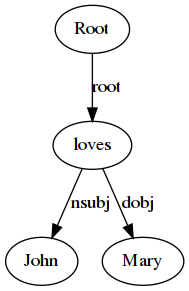
\includegraphics[scale=0.32]{figures/dots/example5_3.png}
\caption{A \textit{John loves Mary.} mondat UD gráfja}
\label{fig:JLM_UD}
\end{figure}


A nyelvtan legfontosabb három művelete a \texttt{forget} (elfelejt), \texttt{rename} (átnevez) és a \texttt{merge} (egyesít). A forget és a rename a jelölések manipulációjára való. A forget művelettel lehet egy jelölést az összes vele megjelölt csúcsról törölni. A rename művelettel egy adott jelölés minden megjelölt csúcson lecserélhető egy másik jelölésre. A merge művelet bemenete az előzőekkel ellentétben két gráf. A bal oldali gráf minden megjelölt csúcsába beszúrja a jobb oldali gráf minden ugyanazzal a jelöléssel megjelölt csúcsát. A műveletek egymásba ágyazhatóak. Csak az egymást követő forget műveletek cserélhetőek fel minden esetben. Forget-et a “f\_ \{\$ jelölés\_ neve \$\}(\{\$ gráf \$\})”
 formában lehet megadni, ahol természetesen a gráf helyén állhat újabb művelet is.  Rename-t pedig a:
\begin{verbatim}
r_{$ régi_jelölés $}_{$ új_jelölés $}( {$ gráf $} )
\end{verbatim}
formátumban lehet megadni. A rename esetén a leváltandó jelölés neve elhagyható és abban az esetben a \texttt{root} jelölésű csúcsokon fogja végrehajtani. A merge formátuma hasonlít leginkább a közismert programozási nyelvek függvényhívásaira: merge(\{\$ gráf1 \$\}, \{\$ gráf2 \$\}) lásd~\ref{sec:example5}.

A példa sok szabálya megfeleltethető a tree interpretáció esetében használttal. Ennek oka az, hogy a nyelvtanokat úgy írtuk meg, hogy azokat könnyű legyen összeilleszteni. Általában a szintaktikai fa egy csúcsát vagy egy három gyermekű csúcsának a felét rakjuk össze egy szabály alatt, és az UD gráfba kerülő élek és a jobb oldali nemterminális szimbólumok szerint nevezzük el a szabályokat. Mivel az UD gráfban és 4lang gráfban sok a hasonlóság, azt is hozzá adom az egyesített nyelvtan példában. lásd~\ref{sec:example6}.

Az s-graph algebra egy jól használható nyelv, de módosítani és javítani is nehéz. Ennek elsődleges oka a bonyolult szintaxis.

A műveletek nehezen átláthatóak. A legtöbb művelet jele egy-egy betű, és így se nem olyan beszédes, mint az aritmetikai operátorok, se nem olyan felismerhető, mint az SGA merge vagy a TTA ‘@’ jelölése. Az operandusok egy részét is a függvény nevében jelölik.  Ez mind sokat ront az átláthatóságon. Sok esetben fölösleges, hogy külön művelet a forget és a rename a merge-től. Egyszerűbb lenne a merge attribútuma ként megadni, hogy a bal oldali gráfból milyen jelölést párosítunk a jobb oldali gráf melyik jelölésével. Azt is lehetne opcionális operandus, hogy a merge után melyik mark legyen elfelejtve.

Ha már a nyelv célja egyértelműen a tömörség, akkor a merge lehetne \textit{‘@’} a TTA-hoz hasonlóan. A forget és a rename is lehetne pl. \textit{‘\&’}, mint reference, \textit{‘\#’}, \textit{‘\%’} vagy egyszerűen egy \textit{‘R’}, ahol a forget egyszerűen egy olyan rename, ahol az új jelölés hiányzik és nem a régi.

A \textit{':'} semmilyen asszociatív viszonyban nincsen az irányított élekkel. A \textit{‘:’}-ot lehetne például \textit{-\{\$ él\_ címke \$\}-}-re cserélni irányfüggően kacsacsőrökkel a végén.
A csúcsok deklarációjában az attribútumok egymástól teljesen eltérő szintaxissal vannak jelölve teljesen feleslegesen. A csúcsok adatai is mehetnének egy szögletes zárójelbe. A zárójelen belül \textit{[n=\{\$ name \$\} , t=\{\$ tag \$\} , m=\{\$ mark \$\}]}formában egyértelmű is lenne, hogy melyik melyik. Így a sorrendjük lehet cserélhető. Így bármelyikük elhagyható anélkül, hogy zavaróvá válna. Itt attribútumok felsorolásáról van szó, így a kisbetű sem zavaró. Adott sorrend mellett a kisbetűk is elhagyhatóak:
\begin{verbatim}
[{$ name $} | {$ tag $} | {$ mark $}].
\end{verbatim}
 lásd~\ref{sec:example7}.

Véleményem szerint ez sokkal tisztább módja lenne és tördelni is sokkal egyszerűbb. Ha az egyik forget vagy rename műveletetre nincs szükség, akkor csak elhagyjuk a hozzá tartozó attribútumokat. Még ennél is szebb lenne, ha a műveleteket operációs jelek jelölnék. lásd~\ref{sec:example8}.

Ugyanakkor ez már túlzottan eltér a gráfleíró nyelvek hagyományos stílusától, és tördelni is nehézkesebb. Operátoros esetben pedig szükség lenne egy sorrendiségre is, ami nem lenne mindenki számára triviális. Arról nem is beszélve, hogy a rename művelet három bemenetű, így nem lehet egy operátorral elvégezni, ahogy az összetett merge négy operátorát is erőltetetten hat.


%----------------------------------------------------------------------------
\section{Az IRTG és az Alto hiányosságai}
\label{sec:shortcomming}
%----------------------------------------------------------------------------
Ebben a fejezetben az IRTG és az Alto hiányosságairól kívánok részletes áttekintést nyújtani, illetve kitérek arra, hogy hogyan lehetne az ezek által okozott problémákat megoldani.
%----------------------------------------------------------------------------
\subsection{Az IRTG hiányosságai}
\label{sec:IRTGshortcomming}
%----------------------------------------------------------------------------

Az IRTG nem egy programozási nyelv, hanem egy nyelvtan. A szabályok egymás alatt adhatóak meg és csak backspace karakterekkel és kommentekkel tagolhatóak. Egy nyelvtan több fájlra nem szedhető szét. A fájl elején fel kell sorolni az interpretációkat, és egyik interpretáció sem hagyható el egyik szabályból sem, még akkor sem, ha semmit sem adnak vissza. A kutatás során egy olyan nyelvtant készítettünk, ami 2700 szabályból áll és négy interpretációból. Ez ha a szabályokat üres sorokkal választjuk el, akkor 16204 sor kódot jelent egyetlen fájlban. Egy ekkora kódot nehéz karbantartani, átlátni, fejleszteni. Tehát szükség van IRTG-ben az importálásra.


Rengeteg esetben a szabályok alig egy-egy szóban térnek el. lásd~\ref{sec:example6}.
Itt a \textit{John} és a \textit{Mary} szóhoz tartozó terminális szabályok között csupán maguk a szavak jelentik a különbséget. A string interpretációban is csak maga a szó jelenik meg. Más szófajú szavak esetében is csak a szabálysort és tree reprezentációt kell még módosítani. Az ilyen esetek miatt nagy kár, hogy az IRTG-ben nem lehet szabályokat egymásból vagy egy közös ősből származtatni.


Sokszor egy szó szófaja egy másik szófaj alkategóriája. Ilyen például az NNP (proper noun, tulajdonnév), ami az N (noun, főnév) alketegórája. Az egy főkategóriába tartozó szófajok sok esetben ugyanúgy viselkednek. Például egy NP-ben, ami egy N-ből és egy JJ-ből áll, minden esetben a két szó között egy \texttt{amod} él lesz az UD gráfban. Ugyanakkor vannak olyan esetek is, amikor az alkategóriáknak csak egy részhalmaza viselkedik hasonlóan. Egy alkategória esetében kétféleképpen lehet megoldani ezt. Az egyik verzióban általánosítunk, tehát az alkategóriákat ugyanúgy kezeljük. Ekkor jelentős áldozatot hozunk a pontosság terén. Más esetben minden egyes alfajra előállítunk minden szabályt, amivel előfordul. Ekkor jelentős áldozatot hozunk hatékonyság terén, mivel sokkal több szabályon kell végigiterálnia az Alto-nak az IRTG futtatásakor. Erre jó megoldás lenne, ha egy szabálysorban minden olyan nemterminális szimbólumot meg tudnánk adni, amire a szabálynak minden interpretációhoz ugyanaz a lépés tartozik. Erre jó megoldás lenne, ha a szabálysorban RegEx-szel lehetne megadni mindegyik jobb oldali nemterminális szimbólumot.


Az IRTG szabályokban mindenre más és más algebrát használunk más és más nyelvvel. Ennek az az oka, hogy mint már az algebráknál részleteztem, minden algebrának vannak hiányosságai. Az IRTG maga lehet önmagában átlátható, de ha az algebrái sokfélék, és némelyiket önmagában is nehéz átlátni, akkor az az IRTG-re is közvetlen hatással lesz (lásd s-graph algebra). Hiába a sokféleség, ha egyes feladatokra csak egy olyan algebra létezik, ami megfelel a célnak és az is erősen korlátozott. Egy algebrára van csak szükség. Egy olyan algebrára, ami az s-graph algebra szintjén van, de átlátható és képes mint a csúcsok sorrendjét kezelni, mint a címkék konkatenációját. Elvégre a szöveg is kezelhető egyetlen csúcsként. Egy ilyen algebrában az is fontos, hogy ne kelljen az egyszerű műveleteket sokkal terjedelmesebben megoldani, mint ha azt az egyszerű algebrákkal végeznénk. Az s-graph javítására az algebra kapcsán mutattam példát, de egy ilyen univerzális algebra már szemantikai változtatásokat is igényelne.


Gyakori az IRTG-ben az, hogy kulcsszavak ütköznek pár változónak a nevével, ami felesleges errort okoz a feldolgozás során. 
Például az \textit{interpretation} szóhoz generált terminális szabályunk ütközött az interpretation szóval, amivel kezdődnek az IRTG fájlok elején az interpretációkat definiáló sorok. 
Ha a szabálynak így kezdődik a neve, akkor már nem fogadja el a futtatókörnyezet. 
Erre a legegyszerűbb megoldás az, ha a nyelvben megjelenik a szöktetés, vagy a kulcsszavakat úgy módosítjuk, hogy ritka speciális karaktereket is tartalmazzanak. 
Például, ha az \textit{interpretation} helyett \textit{<interpretation>} lenne a kulcsszó. 
Persze a problémát az is megoldaná, ha az Alto lexerje kellően intelligens lenne a pozíciófüggő tokenezéshez.

%----------------------------------------------------------------------------
\subsection{Az Alto hiányosságai}
\label{sec:Altoshortcomming}
%----------------------------------------------------------------------------

Az Alto működése iteratív. 
Végigiterál az összes lehetséges levezetési fán a környezetfüggetlen nyelvtanban, és kiválogatja a bemenetre illeszkedőeket. 
Ez alatt persze különböző módszerekkel igyekszik elkerülni azokat a lehetséges levezetéseket, amiről már tudja, hogy biztos rosszak lesznek. 
Erre az egyik legegyszerűbb módszer az, ha a levezetési fákat fentről lefelé generáljuk és kihagyjuk azokat a lehetőségeket, amik már magasabb szinten olyan élet vagy csúcsot vagy azok olyan halmazát vesznek be a derivációba, ami a bemenetben nem szerepel. 
Ezt hívják \textit{optimalizált DFS Parsing}-nak

Az elvi működés és a megvalósítás következtében az Alto rendkívül lassú. 
A feljebb említett 2700 szabályos és négy interpretációs nyelvtan nagyjából 200000 adaton bő 30 óráig futott, pedig a rendelkezésünkre álló tanszéki szerveren futtattuk. 
Ez a mi feladatunk esetében elfogadhatatlan. 
Ezért nem ártana egy hatékonyabb C++ verzió az ilyen méretű munkákhoz. 
Már a C++17 és a hamarosan érkező C++20 is Programozó barát, kényelmes programozási nyelvek.
Nem nehéz az alap platformokon futtatható verziókat legenerálni a nyílt forráskódból. 
Egy könyvtár formájában Pythonból is elérhető lehetne ez a verzió.

Az Alto rengeteg felesleges munkát végez, mivel azokat a megoldásokat is kigenerálja a bemenetből, ami más interpretációk derivációjában errorhoz vezet. 
Az ilyen eseteket is ki lehetne szűrni már a derivációs fa magasabb szintjének az iterációja során. 
Ugyan ez nehezítené a nyelvtanok javítását, mivel nem tudnánk az errort okozó eseteket rendesen kianalizálni, de nem is a nyelvtan javítása során szeretnénk ilyen méretes adathalmazokat futtatni. 
Jó lenne, ha ez opció ként lenne elérhető. 

Az Alto mindennek ellenére a jelenlegi legfejlettebb program az IRTG futtatására, és állandó fejlesztés alatt áll. 
A pontos működését még nem ismerjük. 
A módosítások többsége viszont a belső működés alapos átdolgozását igényli. 
Erre jelenleg még nincs erőforrásunk.

%----------------------------------------------------------------------------
\section{IRTG automatikus generálása}
\label{sec:solutions}
%----------------------------------------------------------------------------
A kutatás során az IRTG-t illető problémák többségét kódgenerálás segítségével küszöböltük ki. 
Két implementáció készült Python nyelven, amik bemeneti adatokból generáltak irtg szabályokat. 
Kezdetben csak NP-k feldolgozása volt a cél, majd onnan terjesztettük ki az implementációkat VP-k és ADJP-k re. 
A generátorkódos megoldások legfőbb hátránya a fejlesztőhöz kötöttség volt. 
Mindkét megoldás a Penn Treebank szintaktikai fáit és az abból a Stanford Parserrel kapott UD gráfokat kapja bemenetként, amiket Python scriptekkel készítettünk elő. 
Ezek a scriptek végezték a fákból a megfelelő kifejezések részfáinak a kiszedését, a részfák rendezését típus szerint és a fák UD gráfjainak a generálását a Stanford Parserrel.

Az első generátort én készítettem el 2018 augusztusában, ez egy objektumorientált megoldás volt. 
Képes volt kommenteket is generálni, kezelni a rövidítéseket és könnyen bővíthető volt, ugyanakkor rush development során keletkezett a szakmai gyakorlatom végén, így a kód még nincsen se letisztázva, se alaposan dokumentálva.

Külön osztályban tárolta a nyers szöveg szavait, a fát és az UD-t, majd ezeket rendezte egy közös osztályba. 
A közös osztály a \texttt{Data}, a nyers szövegé a \texttt{Terminal}, a fáé a \texttt{Tree}, az UD-é és a 4lang-é a \texttt{Dependency}. 
Az összes osztály rendelkezett saját szöveg bemenetű konstruktorral, ami közvetlenül a bemeneti adatok formátumából inicializálja az osztályt.

A \texttt{Terminal} egy szót tárolt és annak a szófaját. 
A \texttt{Tree} tartalmazta a részfát a Stanford Parser formátumában, a TTA formátumában, a TTA formátumában levelek nélkül és külön a szavakat. 
A Tree legtöbb formátuma csak a kommentek generálásához volt hasznos, de ideiglenesen mindegyiket generálta a program a kommentek végleges formátumától függetlenül. 
A \texttt{Dependency} tárolta a fej-szót, a dependens-szót, az él UD típusát és az él 4lang típusát. 
Az UD él 4lang-ra vetítését a \texttt{Fourlang} enum és egy dictionary segítségével végezte. 
Mint korábban említettem, a szavak és 4lang fogalmak megfeleltetésével még mai napig sem foglalkozunk, de az is ebbe az osztályba került volna és feltételezhetően szintén egy dictionary és enum segítségével.

Maga a generálás az adatok függvényében történő szövegkonkatenációból állt.
Minden egyes IRTG típus generálása külön függvényben történt.
A kifejezés generátor függvények először betöltötték az adatokat a \texttt{Data} osztályokba, majd kiszűrte az egyedi adatokat a levél nélküli fák és UD élek alapján. 
A komment első sorát aszerint generálta, hogy van-e kapcsolat a szavak között, és hogy a fej vagy a dependens van-e előrébb. 
Ez a sor azt írta le, hogy milyen kifejezést milyen típusú szavakból épít a szabály és, hogy a dependens milyen szerepet lát el a mondatban. 
Ehhez az adatok rövidítéseit a \texttt{Short2Long} osztály segítségével oldotta fel, aminek a betöltendő adatai  a viszonylag kevés szófaj- és éltípus okán kézzel készültek. 
A következő két komment a szintaktikai fa első példányát tartalmazta a TTA és Stanford Parser formátumában. 

A szabálysort az adatokból nem volt nehéz legenerálni, mivel a szabályok neveit eredetileg is a bemenetek TT interpretációjának gyökere és az UD élek alapján képeztük. 
A string és tree sorok csak a szabály bal oldali nemterminális szimbólumától függenek, így azok konstans szövegek voltak. 
Az UD-nél a szövegbe csak az él nevét kellett beszúrni attól függően más sablonba, hogy a csúcsok között van-e kapcsolat, megjelenik-e mindkettő a 4lang gráfban (a \textit{the},\textit{a} és \textit{an} szavak például nem), és hogy ha van köztük kapcsolat, akkor melyik a fej. 
A 4langnak ezek a tulajdonságok már bele voltak kódolva az enum alapú típusába, így itt csak egy else-if ágazaton kellett végigmenni (mivel Pythonban nincsen switch case).

Már itt is látszott, hogy számos lehetőség van optimalizációra. 
Például a kódba ágyazott adatokat is ki lehetett volna szervezni txt fájlokba. 
Így a fourlang if-else ágai is megoldhatóak lettek volna egy dictionary-vel és karbantarthatóbbak lettek volna az adatok. 
A kettő magas kifejezések részfái között rengeteg volt a hasonlóság, így könnyedén össze lehetett volna a generáló függvényeiket vonni. 
A magasabb kifejezés részfákat se lett volna sokkal nehezebb ugyanabban a függvényben generálni. 
Az adatok feldolgozását és tárolását egy osztályban is meg lehetett volna oldani. 
A könnyen származtatható adatokat, mint a fák Stanford formátuma és és a 4lang részgráf típusok, nem kellett volna eltárolni. 
Elég lett volna, ha a többi adatból származtató függvényeket is tartalmazza az egy darab \texttt{Data} osztály. 
Ezzel azt a duplikációt is elkerülhettük volna hátrány nélkül, hogy a terminálisokat majdnem mindegyik adatstruktúra eltárolta.

Végeredményben viszont még ekkor is egy olyan programunk lett volna, ami az IRTG kódot csak generálja. 
Végső soron template-elést használt volna, de az IRTG nyelvhez kötött szinten. 
Az új szabályok egyre több kódot jelentettek volna, és nehéz lett volna a hibákat meghatározni bárkinek, aki nem dolgozott a program elkészítésén és nem tanulmányozta hosszabb ideig.

Jelenleg egy másik programmal generálunk IRTG-t, amely szintén a Penn Treebank-formátumú fák és dependenciaparszolt változatuk összehasonlítása alapján állítja össze a szabályokat. 
Futása során az egyes dependenciákhoz tartozó szavakat reprezentáló leveleket kikeresi a fából, majd ezek közös őse és a levelek felé vezető út mentén található közvetlen leszármazottak konfigurációja alapján hozza létre a megfelelő IRTG szabályokat.

Az általam fejlesztett nyelv, a \texttt{Slime} első verziója nem lesz képes gráfműveletekre, de könnyű lesz benne olyan kódot készíteni, ami mindenki számára érthető, mindezt minimális overhead-del.
Csak a bemeneti adatokat szükséges generálni hozzá. 
Mivel az alkategóriákon belül a legtöbb szabály összevonható lesz RegEx és template-elés segítségével, a sorrend sem jelent majd problémát.
Jelenleg úgy tűnik, hogy a teljesen hatékony megoldás a Slime és a jelenlegi generátor kombinációja..

%----------------------------------------------------------------------------
\chapter{A Slime nyelv}{\href{https://github.com/Hollo1996/SlimeAnUTLE}{A Slime nyelv}\footnote{\url{https://github.com/Hollo1996/SlimeAnUTLE}}}
\label{sec:Slime}
%----------------------------------------------------------------------------
\section{Bemutatkozás}
\label{sec:SIntro}
%----------------------------------------------------------------------------
A szakdolgozat keretében kifejlesztett nyelv a Slime nevet kapta.
A Slime egy UTLE (Universal Templater Language Extension), 
avagy egy más nyelvek fölé szánt univerzális bővítmény, ami template-elést használ.

A fejlesztés során az IRTG kiegészítése az elsődleges cél, de ezt a sok iteráció alatt kinőtte a koncepció. 
Ennek több oka volt. 
Először is az IRTG-nek a legtöbb hiányossága későbbi fejlesztés során megszűnhet a nyelv kiegészítésével (Lásd fejezet ~\ref{sec:SStatesOfDevelopment}).
A kiegészítéshez a belső működés módosítására nincs feltétlen szükség. 
Az ALTO-t ugyan viszonylag könnyű kiegészíteni és módosítani, mivel kellően objektum orientált és nyílt forráskódú,
ugyanakkor állandó fejlesztés alatt áll, ezért a forráskód módosítása és kiegészítése is verzió követést igényel. 
A függőséggel arányosan nő a karbantartási költség. 
Az ALTO fejlődésével pedig sok kód feleslegessé válik. 
Ezért külső megoldás kell. 
Minden nyelv fejlődik, de mindig lesznek fejletlen nyelvek is, amik felett a Slime hasznos lesz.

Programozási és adat leíró nyelveknek széles rétege alul fejlett. 
Ennek egyik válfaját alkotják azok a nyelvek, amik még fiatalok, és egyszerűen nem jutottak még el a kellő érettségig. 
A másik válfaj pedig azok a nyelvek, amiknek túlzottan célorientáltak a bennük rejlő lehetőségekhez képest.
A fejlesztőknek sokszor nem éri meg az összes alap funkcionalitást implementálni. 
Jó kérdés, hogy az IRTG a két kategóriából melyikbe esik vagy nem esik. 
A Slime küldetése az, hogy ezeket a nyelveket felemelje egy magasabb szintre azok módosítása nélkül. 
Növelje a kódok átláthatóságát, struktúráltságát, és kiírtsa a repetitív kódrészeket.

Az univerzalitást szem előtt tartva egy olyan módszert kell alkalmazni, ami független a kiegészített nyelv fordítójától és szintaxisától. 
Erre a legpraktikusabb megoldás a template-elés. 
Először a kiegészített nyelvre generáljuk a kódot és azt futtatjuk a nyelv saját fordítójával. 
Ez ugyan egy új lépést jelent, de párhuzamosítással áttetszővé válhat a Slime könnyű súlya miatt. 
Az ötlet persze nem teljesen egyedi. 
Eddig is sokféle template processzort és enginet használtak(Lásd fejezet~\ref{sec:SAlternatives}) adatleíró nyelvekhez. 
Ugyanakkor ezek inkább könyvtárak, mintsem nyelvek.
Legtöbbször egy magasabb szintű nyelvből lehet kezelni őket, amiknek a támogatása is szükséges. 
Céljuk tipikusan HTML vagy épp CSS kódok folytonos manipulációja. 
A Slimeból sem nehéz könyvtárat készíteni, de hosszú távú célja az abszolút önállóság. 
Kerüli a függőséget minden felette lévő rétegtől is.

A réteges architektúra és egyirányú viszony okán a kiegészített nyelvre \textit{alárendelt nyelv}ként (subordinate language) fogok hivatkozni.
A templatek esetében megszokott terminológia ``master document''-ként hivatkozik az alárendelt nyelv sablonjaira.
Ezzel ellentétben én \textit{alárendelt dokumentum}ként (subordinate document) fogok hivatkozni rá. 

A Slime fiatal, így a Slime-ban is megjelennek még azok a jelenségek, amiket elkerülni igyekszik. 
Nem haladja meg azt a funkcionalitást, amire tervezve lett. 
Közel sem Turing teljes. 
Csak a templateléshez és struktúráláshoz szükséges alapfunkciókat implementálja (Lásd fejezet ~\ref{sec:SStatesOfDevelopment}). 
Nem tartalmazza a legalapvetőbb aritmetikai műveleteket sem. 
A kódjában legtöbbször könnyű, de nem mindig elkerülhető a repetitivitás. 
Még hosszú út áll előtte. 
Ezekre a problémákra és tervezett megoldásaikra a későbbiekben fogok kitérni. 
A Slime így is jelentős fejlődést jelent olyan nyelvek számára, amikben a tünetek sokkal súlyosabban jelentkeznek. 
Ilyen nyelv az IRTG, HTML, XML és irónikusan annak az ANTLR-nek a lexer és parser nyelvtan leíró nyelve, amit a Slime jelenlegi fordítója használ (lást Példák ~\ref{sec:SEIRTG}). 
Tehát végső soron a Slime egy olyan nyelv, ami saját magának az implementálását is határozottan könnyebbé tette volna.


%----------------------------------------------------------------------------
\section{Tervezési szempontjai}
\label{sec:SDesign}
%----------------------------------------------------------------------------
A Slime a következőkre összpontosít:
\begin{itemize}
\item alárendelt és fölérendelt nyelvtől való függetlenség
\item könnyű súly és sebesség
\item platformfüggetlenség
\item könnyű bővíthetőség
\item esztétikum és egyéniség
\item kód átláthatósága és könnyen érthetősége
\item szabad tördelhetőség akár több fájlba
\item enyhe tanulási görbe
\item hatékony programozás az alárendelt nyelven
\end{itemize}

Eddig a nyelvektől való függetlenség volt a legalaposabban tárgyalva. 
A nyelv külön fordítót, templatelést és szöktetést használ e célból.

A könnyű súlyt könnyen parszolható szintaxissal és egyszerű műveletekkel támogatja. 
Később a túlsúlyos külső könyvtárak elhagyása is sokat fog segíteni.

A platformfüggetlenség okán Kotlinban készült az első fordító, ami JVM-en fut. 
A könnyen bővíthetőséget modularitással és egységes szintaxissal támogatjuk.

Az esztétikum és felismerhetőség is első sorban a szintaxisra vonatkozik. 
Itt a legfontosabb az átláthatóság. 
Fontos, hogy szép kódunk legyen, amiben a nyelvi elemek jól felismerhetőek.
Ugyanakkor az is fontos, hogy a Slime kódja kitűnjön az alárendelt nyelv kódjából. (lásd fejezet ~\ref{sec:SBaseSyntax})

A szabad tördelhetőségben segítenek sokat a zárójelek, változók és az importálás megvalósítása. (lásd Példák ~\ref{sec:SEIRTG}) 
A könnyen tanulhatóságot a beszédes, de tömör jelölések, kevés, de sok oldalú műveletek és következetes működés és a kódok átláthatósága is segíti.

A hatékony programozást a tömörített kifejezések és a szükségtelen jelölések elhagyása segítik.

Sokszor kellett kompromisszumokat kötni a szempontok között. 
Ezeket a döntéseket ugyanakkor legtöbbször inkább elkerültük. 
Fontos rugalmasnak lenni, és engedni a programozót a saját stílusát követni. 
A nyelv hemzseg a zárójelektől a könnyű parszolás és átláthatóság érdekében.
Ugyanakkor vannak biztosítva módszerek a csukó zárójelek esetenkénti elhagyására.
Sok nyelv az adatot elkülöníti a kódtól. 
Slimeban a kód tartalmazza a templatet, de külön fájlba szervezéssel elkülöníthető. 
Más templater engine-k könyvtáraival ellentétben nem a Slime-ba ágyazzuk az alárendelt nyelv kódját. 
Az alárendelt nyelv kódjába ágyazzuk a Slime-ot. 
Így a Slime használatának mennyisége teljesen opcionális. 
A felhasználó hagyatkozhat teljesen a Slime-ra, vagy használhatja csak a legrepetitivebb kód részek esetén. 
A Slime esetén akár saját maga is könnyen lehet az alárendelt nyelv. 
Ezt a szöktető zárójelek nagyban segítik. 
A reguláris kifejezések(RegEx) esetén például csak egy karaktert lehet szöktetni, így a RegEx-xel RegEx-ben keresni elég nehézkes.
Ilyenkor ugyanis minden speciális karaktert szöktetni kell. 
Slime esetében az alárendelt Slime kód részeket egyszerűen \{” ”\} szöktető zárójelek közé rakjuk.


%----------------------------------------------------------------------------
\section{Alternatívák template-elésre }
\label{sec:SAlternatives}
%----------------------------------------------------------------------------
Rengeteg alternatíva létezik template-elés terén.
Az itt felsoroltak csak egy ízelítő belőlük.
Azt kívánom szemléltetni velük, hogy a ma fellelhető megoldások miben térnek el a Slime-tól.
Nem kívánom a nyelveket kritizálni.
Más a céljuk, így természetes, hogy nem tudnak a Slime célkitűzéseinek eleget tenni.

%----------------------------------------------------------------------------
\subsection[Mustache]{\href{https://mustache.github.io}{Mustache}\footnote{\url{https://mustache.github.io}}}
\label{sec:mustache}
%----------------------------------------------------------------------------
A Mustache az egyik legtöbb forrással rendelkező templater könyvtár.
Tömbnyire HTML manipulációra használják.
Elérhető többek között Ruby, JavaScript, Python, PHP, Perl, Objective-C, Java, C\# /.NET, Android, C++, Go, Lua, Scala, Delphi, R, C nyelveken.
A 46 nyelv teljes listája elérhető a hivatalos GitHub oldalukon.
A Kotlin ugyan még nem szerepel benne, de ami Java alatt elérhető, az Kotlin alatt is.
Jól működik többek között a TextMate, Vim és Emacs szövegszerkesztőkkel.

Un. \textit{logic-less template}-eket használ.
Ez annyit tesz, hogy elkülöníti a logikát és a a sablonokat.
A mezőket dupla kapcsos zárójelekkel jelöli; például: \texttt{Dear \{\{ name \}\}}.
A mezőkre \textit{tag}-ként hivatkozunk esetében.
A \textit{name} a tag kulcsa.
Ezt a kulcsot fogom használni a későbbi példáimban is.

A templatbe kulcsérték párokat lehet beszúrni.
Minden tag-be az ő nevéhez tartozó adat szúródik be.

\todo{Néhány tipp:
  \begin{itemize}
    \item Légyszíves minden (rövid) példát, kódot rakj \texttt{\textbackslash texttt}-be, ahogy én is raktam fent!
    \item Kulcsszavak, elnevezések bevezetésekor nyugodtan rakd őket italics-ba!
    \item A bemutatott nyelvekre rövid példa, ha lehet! Még jobb, ha ugyanazt mutatod meg az összes nyelvben.
  \end{itemize}
}

Több fajtája létezik a tag-eknek:
\begin{itemize}
\item \emph{Variables:}
Ezek a legalapabb tag-ek.
Amikor a template name kulcsú tag-jébe szúrunk bele, akkor az összesbe szúrunk bele.
Alapvetően szöktetve vannak a HTML-ből.
Például a \textit{<b>GitHub</b>} helyett \textit{\& lt;b\& gt;GitHub\& lt;/b\& gt;} kerül a kódba.
Ha szeretnénk, hogy ne legyenek szöktetve, akkor \textit{\{\{\{ name \}\}\}} vagy \textit{\{\{\& name \}\}} módra kell megadnunk őket.
Például ha a \textit{\{\{\{name\}\}\}} vagy \textit{\{\{\& name\}\}} mezőbe szúrjuk be a \textit{<b>GitHub</b>} szöveget, akkor az \textit{<b>GitHub</b>} ként is lesz beszúrva.
\item \emph{Sections:}
Egy section tartalma egy vagy többször is megjelenhet.
Elejét \textit{\{\{\# name \}\}} és végét \textit{\{\{/ name \}\}} módra jelöljük.
A kettő között egy sablon részlet található.
Egy boolean értéket vagy adat listát lehet a section mezőbe szúrni.
Ha false-t vagy üres listát kap, akkor nem jelenik meg.
True esetén megjelenik egyszer és a tagjeibe a kulcsukhoz tartozó adatot szúrja be.
Nem üres lista esetén a belső sablonba a lista minden elemét beszúrja és az eredményeket egymás alá írja ki.
Ha egy paraméter nélkül hívható objektumot adunk át neki, akkor azt meghívja és a kimenetét szúrja be a Section helyére.
Ez lehet lambda kifejezés, funktor vagy function is.
\item \emph{Inverted Sections:}
Elejét \textit{\{\{$\cap$ name \}\}} és végét \textit{\{\{/ name \}\}} módra jelöljük.
Akkor jelennek meg, ha a kulcsuk a kapott adatban nem létezik, false vagy üres lista.
Ez például hiányzó kulcsok esetén alkalmas hiba üzenet vagy más visszajelzés megjelenítésére.
\item \emph{Comments:}
Mustache-ben kommentet \textit{\{\{! ignore me \}\}} formátumban írhatunk.
Ezeket bárhol kezdhetjük a szövegben, de nem kerülhetnek tag-be.
\item \emph{Partials:}
A \textit{\{\{> name\}\}} formátumban adhatóak meg.
Rekurzívak is lehetnek, ha nem tartalmaznak végtelen ciklust.
Ezzel valósítja meg a mustache az importálást.
A felső példa például a name nevű mustache fájl tartalmát jelöli.
\item \emph{Set Delimiter:}
Ezzel a funkcióval új jelölés vezethető be a dupla kapcsos zárójelek helyett.
Például a \textit{\{\{=<\% \%>=\}\}} a \textit{\{\{ name \}\}} formátumot \textit{<\% name \%>}-re cseréli.
Ez hasonló módon vissza is állítható: \textit{<\%=\{\{ \}\}=\%>}
Ez a Mustache megoldása arra, hogy váratlan szintaxisú környezetben is jól használható legyen.
\end{itemize}

Összegezve, a Mustache egy egyszerű, kreatív és egyszerű templater engine.
Ugyanakkor külső vezérlést igényel működéséhez és HTML-ekre van szakosodva.
Nincs szöktetés, csak a tag-ek jelölése állítható dinamikusan.
Ez ugyanakkor egy olyan képesség, amivel a Slime nem rendelkezik (még). 



%----------------------------------------------------------------------------
\subsection[Jade]{\href{https://pugjs.org/api/getting-started.html}{Jade}\footnote{\url{https://pugjs.org/api/getting-started.html}}}
\label{sec:jade}
%----------------------------------------------------------------------------
A Jade az egyik legelterjedtebb templater nyelv.
2017-ban át lett nevezve pug-gá és az új források is már így hivatkoznak rá.
Ennek ellenére legtöbben még az eredeti nevén ismerik.

Erősen HTML-re van szakosodva.
A HTML nyitó jeleket egyszerűbben lehet benne írni.
És a csukó jel teljes mértékben elhagyható.
A tag-ek jelölésére a \#\{ name \} jelölést használja.

attribútumok:
\begin{verbatim}
<a ...> ... </a> 
\end{verbatim}
helyett 
\begin{verbatim}
a(...) ...
|
|
\end{verbatim}
Utóbbi esetben a két \textit{'|'} zárja az \textit{a}-t.

Elágazás is lehetséges benne: body(class=authenticated ? 'authed' : 'anon')

A zárójelekben az elemeket enterrel tagolja:
\begin{verbatim}
input(
  type='checkbox'
  name='agreement'
  checked
)
\end{verbatim}

"-" jellel javascript is ágyazható bele.

class adható meg egyszerűen így is:
\begin{verbatim}
a.button
\end{verbatim}

Hosszasan lehetne sorolni a szintaxis belüli változtatásokat és javascript trükköket.
Összegezve a pug egy nagyon fejlett és összetett nyelv.
Erősen javascriptre és HTML-re van szakosodva.
Előtérbe a hatékony kódolást helyezi az átláthatósággal szemben.


%----------------------------------------------------------------------------
\subsection[Underscore Templates]{\href{https://underscorejs.org}{Underscore Templates}\footnote{\url{https://underscorejs.org}}}
\label{sec:underscore}
%----------------------------------------------------------------------------
Onnan kapta a nevét, hogy minden függvény az \_ névtérből érhető el.
(Én magam is sokszor használtam saját hasonló nevű Java handler osztályokat, hogy átláthatóbbak legyenek a műveleteim. 
\_ nevű osztályokat persze a Java újabb verzióiban már nem lehet létrehozni.)
Az Underscore nem csak templatelésre való.
A hivatalos oldalán azzal kezdi, hogy ez egy javascript library.
Más alatt nem is elérhető és nem kíván teljes nyelv lenni.
Több mint 100 függvényt kínál fel.
Funkcionális segédként tartalmaz map-et, filter-t és invoke-ot.
Ezen kívül tartalmaz function binding-ot, javascript templating-et, quick index-ek készítését, deep equality testing-et.

A templatelésre is számos ügyes megoldást tartalmaz.
<\% name \%> formátumban jelöli a mezőket.
Ennek is több verziója van, amit a mezőt megelőző karakter jelöl:
\begin{itemize}
\item \emph{<\%=name\%>:}
Ezt interpolate-nak hívják. 
Ez a legalapvetőbb mező.
A beszúrt adatot egy az egyben beszúrja.
\item \emph{<\%-name\%>:}
Ezt escape.nek jóhívják.
A beszúrt adat \texttt{\& < > " ' /} karaktereit HTML skipp-eli.
\item \emph{<\%name\%>:}
Ezt evaluate-nek hívják.
Javascript kódrészleteket lehet beleszúrni.
Például egy foreachet, ami egy listányi adaton végig megy és mindegyiket beleszúrja a mezőkbe, mindegyik beszúrással új példányt hozva létre.
Alkalmas elágazások implementálására is.
Képes metadatokat elérni.
\end{itemize}

A szintaxis is állítható:\_ .templateSettings = \{interpolate : /$\backslash$ \{$\backslash$\{(.+?)$\backslash$\}$\backslash$\}/g \};

(érdekesség: A mustache hivatalos példáiban azt mutatják be, hogy hogyan lehet az Underscore mező nyitó és csukó zárójeleit használni a mustache helyett a \textit{\{\{=<\% \%>=\}\}} segítségével. Mint feljebb látható, az Uderscore hivatalos példáiban épp a mustache nyitó és csukó zárójeleire váltunk.)

Az Underscore a Mustache és a Jade(Pug) szemléletét ötvözi.
Több féle mezőt használ, de megengedi a javascript elemek beszúrását.
Ezzel pedig bevállalja, hogy a JavaScript-tel erős függőségben legyen.
Ez persze JavaScript alatt a legelőnyösebb megoldás.
A lehető legkevesebb új információ mellett lehet hatékonyan template-lni.
Engedi a szintaxis átállítását is, ami mindig hasznos, ha nincsen a nyelvben hatékony skippelés.

%----------------------------------------------------------------------------
\subsection[Embedded JS Templates]{\href{https://github.com/mde/ejs}{Embedded JS Templates}\footnote{\url{https://github.com/mde/ejs}}}
\label{sec:embedded}
%----------------------------------------------------------------------------
Ez is egy könyvtár.

Jelölése az Underscore-ra hasonlít.
Tele van hasznos funkciókkal.
\textit{<\% \%>}-tel JavaScript ágyazható vele, amivel könnyen megvalósíthatóak vezérlési szerkezetek (ciklusok, if-ek, stb.).
\textit{<\%= \%>} szöktetett beszúrás végezhető. 
\textit{<\%-  \%>} szöktetés nélküli beszúrás.
Tehát pont fordítva, mint az Underscore esetében.
Newline-trim mód, ha \textit{-\%>} -kal zárjuk.
\textit{<\%\_  \_ \%>}-szel Whitespace-trim mód a Control Flow számára. 
Saját határoló jelek is bevezethetőek (pl.: \textit{<? ?> <\% \%>} helyett).

további jelölései:
\begin{itemize}
\item \emph{\textit{<\%} :} 'Scriptlet' tag a control-flow-nak.
\item \emph{\textit{<\%\_} :} 'Whitespace Slurping' Scriptlet tag, elhagy minden whitespace-t maga előtt.
\item \emph{\textit{<\%=} :} beszúrja az adatot HTML szöktetve.
\item \emph{\textit{<\%-} :} beszúrja az adatot HTML szöktetés nélkül.
\item \emph{\textit{<\%\#} :} kommentelés
\item \emph{\textit{<\%\%} :} Egy \textit{'<\%'}-t ad vissza
\item \emph{\textit{\%\%>} :} Egy \textit{'\%>'}-t ad vissza
\item \emph{\textit{\%>} :} Egyszerű csukó tag
\item \emph{\textit{-\%>} :} Trim-mode ('newline slurp') tag, az utána jövő új sor karaktereket elhagyja.
\item \emph{\textit{\%>} :} 'Whitespace Slurping' csukó tag, elhagy minden whitespace karaktert maga után.
\end{itemize}

Nagy hangsúlyt fektet a whitespacek kezelésére.


%----------------------------------------------------------------------------
\subsection[HandlebarsJS]{\href{https://handlebarsjs.com}{HandlebarsJS}\footnote{\url{https://handlebarsjs.com}}}
\label{sec:hjs}
%----------------------------------------------------------------------------
Ez a megoldás a mustache működéséhez és jelöléseihez közelít.
Handlebar-ként hivatkozunk a HandlebarsJS mezőire.
A böngészőbe <script> blokkban lehet bevinni.


Handlebar-oknak sok fajtája létezik:
\begin{itemize}
\item \emph{\textit{\{\{ name \}\}} :} 
Alap Handlebar.
HTML szöktetést használ.
\item \emph{\textit{\{\{\{ name \}\}\}} :} 
Handlebar HTML szöktetés nélkül.
\item \emph{\textit{\{\{\# list name\}\} ... \{\{/list\}\} }:} 
blokkos kifejezés.
Például ebben az esetben egy nema címkéjű lista.
Egy listányi adatot beleszúrva mindegyikkel elvégzi a beszúrást és egymás alá listázza az eredményt.
\item \emph{\textit{\{\{! ... \}\} ... \{\{--! ... --\}\}} :} kommentelés
\end{itemize}


%----------------------------------------------------------------------------
\subsection[Smarty]{\href{https://www.smarty.net}{Smarty}\footnote{\url{https://www.smarty.net}}}
\label{sec:smarty}
%----------------------------------------------------------------------------
A smarty egy rendkívül fejlett templater engine.
Mint a legtöbb templater, PHP-ra és  HTML-re szakosodott.
A blokkjait kapcsos zárójellel határolja.

Számos funkcionalitást lehet vele a templaten belül jelölni.
Ezeknek részletezése nem fér bele a szakdoga kereteibe, így csak a szintaxis szemléltetésének céljával sorolok fel nyelvi elemeket:

\begin{itemize}
\item \emph{variable: }
\textit{\{\$ name \}}
A Smarty mezői.
Ugyanakkor sokkal fejlettebbek annál.
Ők maguk is tartalmazhatnak más változókat. 
\item \emph{functions: }
\textit{\{funcname attr1="val1" attr2="val2"\}}
\item \emph{komment: } 
\textit{\{* This is a comment *\}}
\item \emph{import: } 
\textit{\{include 'page\_footer.tpl'\}}
\item \emph{cycle: }
\begin{verbatim}
<tr class="{cycle values="odd,even"}">
   <td>{$data[rows]}</td>
</tr>
\end{verbatim}
A ciklus megvalósítása. 
Végig iterál az értékeken.
\item \emph{upper: } 
\textit{\{\$name|upper\}}
Nagy betűkkel szúrja be a szöveget.
\item \emph{foreach: } 
\begin{verbatim}
{foreach $nameList as $name}
    <li>{$name}</li>
{/foreach}
\end{verbatim}
Loops throw the whole array.
Egy fejlett megoldás, ami sok féle képpen használható.
Nem részletezem a szakdoga kereteiben.
\item \emph{display: } 
kiír konzolra egy templatet.
\end{itemize}

Összefoglalva a Smarty minden műveletet kapcsos zárójelekbe zár.
Ezeket figyelmen kívül hagyja, ha whitespace-be vannak foglalva.
A föggvények nevét a kapcsos zárójelekkel jelöli.
Igyekszik mindent saját nyelvi elemekkel megoldani.
Érdekes, hogy a Smarty ismerete nélkül, a slime szintaxisa is ebbe az irányba mozdult el.
A Smarty egy rendkívül fejlett és tartalmas nyelv.
A Slime ennél egy sokkal egyszerűbb megközelítést követ.

%----------------------------------------------------------------------------
\section{Az Slime alapjai}
\label{sec:basics}
%----------------------------------------------------------------------------
Nincs nyelv, amiben könyebb "Hello World"-öt írni, mint Slime-ban!
Csak leírod, és a kimenetben benne lesz.
A Slime egy letisztult nyelv. 
Összesen tizenegy példányosítható típust és tíz műveletet tartalmaz. 
Egységes és csak erősen indokolt esetekben tér el a természetes, bevett megoldásoktól.
A továbbiakban a szintaxist, típusokat és műveleteket bonyolultság szerinti sorrendben igyekszem leírni.
Először a szintaxis alapjait írom le.
Utána az absztrakt őstípusokkal folytatom.
Ezt követően bemutatom a sablon deklaráláshoz szükséges típusokat.
Ezt követően mutatom be az alap műveleteket,
majd folytatom a tároló típusokkal.
A hatodiktól a nyolcadik alfejezetig arról írok, hogy a Cont osztályokon hogyan végezhetőek műveletek.
Ezt követi a név manipuláció.
Végezetül bemutatom a haladó szintaxist.

  

%----------------------------------------------------------------------------
\subsection{Alap Szintaxis}
\label{sec:SBaseSyntax}
%----------------------------------------------------------------------------
A szintaxis terén volt a legnehezebb megtalálni a hangsúlyt a tömörség, az átláthatóság és a tanulhatóság között. 
Fontos volt az, hogy a jelölések már bevettek legyenek vagy következetesek, hogy könnyű legyen tanulni. 
De az átláthatósághoz az is fontos volt, hogy a jelölések egyediek legyenek

A bevett jelölésekhez népszerű templater enginek, a Kotlin és más C alapú nyelvek szolgáltak alapul.
\begin{itemize}
\item \emph{sablon nyelvek:}
A Smarty-hoz hasonlóan (Lásd fejezet ~\ref{sec:smarty}) a parancsokat az alárendelt kódba ágyazzuk.
Minden művelet kapcsos zárójelbe kerül, hogy elkülönüljön az alárendelt kódtól.
Ez rendes tördelés mellett az átláthatóságot is segíti, és használatával a műveleti sorrend is egyértelmű. 
A Mustache-hoz hasonlóan (Lásd fejezet ~\ref{sec:mustache}) a blokkok típusát a blokkon belül jelöli egy-két karakterrel.
Ez is segíti az alárendelt kódtól való elkülönülést.
Igaz Slime esetén a csukó zárójel előtt is jelöljük a blokk típusát az átláthatóság kedvéért.
\item \emph{Kotlin:}
Deklarációnál a név, típus érték sorrendet követi.
Ekkor a nevet és a típust kettősponttal választja el.
\item \emph{C alapú nyelvek:}
A több parancsot tartalmazó zárójelekben(Lásd bővebben ~\ref{sec:SAdvaSyntax}) a parancsokat pontosvesszűvel választjuk el.
A zárójeleken belül az attribútumokat vesszővel és kettősponttal választjuk el.
A \textit{':'} választja el a függőségben lévő attribútumokat és a \textit{','} a függetleneket. 
Például a kulcs érték párokat \textit{':'} köti össze.
Ha az attribútumok között összetettebb hierarchia van, azt a kettőspont mellett kerek zárójelek is jelölik. 
A referenciát a \textit{'\&'} karakter jelöli.
\end{itemize} 
Egyes műveletek esetén a főbb attribútum halmazokat saját operátorral is elválasztjuk. 
Például deklaráció során a létrehozott változó metaadatait(nevek és típus) az attribútumaitól egy “:=” operátor választja el.
A következő fejezetek példái jól szemléltetik ezeket is.

%----------------------------------------------------------------------------
\subsection{Vari őstípus}
\label{sec:SVariSuper}
%----------------------------------------------------------------------------
A Slime egy erősen típusos nyelv.
Nincsen benne öröklődés, de van két absztrakt ős típus.
A Slime összes típusának közös absztrakt őstípusa a Vari(variable).

Minden Vari példánynak lehet akár több, akár nulla neve.
Ezek a nevek az angol ábc kis-nagy betűit, alulvonást és számokat tartalmazhatnak. 
Számokkal ugyanakkor nem kezdődhetnek.
Egy névtelen változó csak az őt birtokló változókon keresztül érhető el.
A több név több esetben is hasznos lehet.
Például az éppen többet használt változókat hivatkozhatjuk a rövidebb nevükön.
Ritkább használat esetén pedig hivatkozhatjuk őket a hosszabb nevükön.
Tömören programozunk, és mindig mindent elérünk egyszerre.
A programozási környezetek gyakran tartalmazzák az automatikus rendezés funkciót.
Egy Slime környezet lehetővé tehetné, hogy a változó meghivatkozásainál a nevét a leghosszabbra cseréli.
Így a programozó gyorsan kódol és néhány gombnyomásra érthetővé teheti a gyorsan leírt kódot.
Vagy például többen dolgoznak egy projekten, de mindenki más terminológia szerint dolgozik.
Ilyenkor mindenki hozzáadhatja a változókhoz azt a nevet, ami neki otthonos.
A nevek teljes mértékben elvannak egymás mellett.

A Slime-ban van importálás.
Az importált fájl változói a fájl változójának nevén, mint namespacen keresztül érhetőek el.
Például az f1 néven importált fájl v1 változója f1.v1 néven érhetőek el.
Ez fontos ahhoz, hogy elkerülhessük a váratlan névütközéseket.
Egy változóhoz nevek később is adhatóak a Name típus segítségével (Lásd fejezet~\ref{sec:SName}).
Az új nevek annak a Slime fájlnak a namespace-éhez fognak tartozni, amelyikben hozzá lettek adva az adott változóhoz. 
Így lehet például egy importált fájl változóit könnyebben elérhetővé tenni.
Ha egy név már foglalt az adott fájlban, akkor egyszerűen felülíródik.
Ekkor a környezet persze dobna warningot.
A több név gyakorlatilag a referenciákat helyettesíti.
Ugyanakkor ez egy sokkal magasabb szintű megoldás.
A változó is tudja, hogy honnan érhető el és milyen név szerint.

Minden Vari-nak létezik a következő négy attribútuma:

\begin{itemize}
\item \emph{names:} 
A változó nevei a fájl elérése szerint.
\item \emph{self:} 
A változó maga. 
Ez a "referencia" helyett magára a változóra hivatkozik.
Ha egy változó közvetlen elérhető, akkor a meghivatkozása nem tartalmaz pontot.
Bizonyos esetekben a parszer az ilyen meghivatkozást Name típusú változónak tévesztheti.
Például, ha egy listát készítünk, és vesszővel felsoroljuk az elemeit (Lásd fejezet~\ref{sec:SContDecl}).
Ilyenkor a self attribútummal egyértelműsíthetjük, hogy a változó elérésre gondoltunk, és nem Name típusú változóra. 
\item \emph{copy:}
Ez az attribútum a változóból egy új másolatot ad vissza név nélkül.
Későbbiekben a copy-ból három féle fog létezni. 
A copyS sekély, a copyD mély és a copy\{\$integer\$\} adott mélységű másolatot fog visszaadni.
\item \emph{type:}
Ez az attribútum jegyzi a változók típusát.
Egy Type típusú változó, ami a változó itt felsorolt négyen túli attribútumait jegyzi.
Ez a változó név szerint nem érhető el, csak vele rendelkező osztályokból.
Ennek célja, hogy az alap típusok ne szennyezzék a kiindulási fájl a namespace-ét.
\end{itemize}

Ezen kívül egyes típusoknak vannak további attribútumai, de metódusai nincsenek. 
Csak a mindenkin végrehajtható operációkat kezelik le másképp. 
Ez a négy operáció a:
\begin{itemize}
\item \emph{deklaráció:} 
Egy új változó létrehozása az adott típussal.
Nem csak ezzel a művelettel lehet változót létrehozni, de ez a legsokoldalúbb módszer rá.
Minden típus példányosítható vele.
A változó nevei is megadhatóak egyből.
Képes más műveletek kimenetéből példányosítani.
\item \emph{törlés:} 
Törli egy változónak az egyik nevét vagy elveszi egy birtokosától.
Egy változó csak akkor szabadul fel, ha az összes nevéről törlik és senki sem birtokolja.
Ha egy változó self attribútumára hívnak törlést, akkor az összes neve szerint törli magát az összes Slime fájlból.
Ugyanakkor a birtokosai továbbra is elérik.
Akkor lehet igazán hasznos, ha nagyon nagy szöveghalmazzal foglalkozunk, vagy le akarunk tiltani ideiglenesen létrehozott neveket.
\item \emph{hozzáadás:}
A hozzáadás egy sokoldalú művelet. 
Ez végez ugyanis minden konkatenációt, beszúrást és deklaráció utáni értékadást.
\item \emph{kiterjesztés:}
A kiterjesztés a C nyelvek ToString műveletének felel meg. 
Szöveggé alakítja a változókat.
Ugyanakkor az alárendelt nyelv kódjába ágyazva beilleszti a változó szöveges értékét az alárendelt nyelv kódjába. 
Ebből az extra funkcionalitásból származik a neve is.
\end{itemize}

Ezek a műveletek nyilvánvalóan alap követelményei a sablon kezelésnek. 
Ha nem tudunk sablonokat létrehozni, beszúrni egymásba és kiírni, akkor nem látjuk el a nyelv alap funkcióit.
A törlés persze másodlagos, de igazán nagy adathalmazok esetén hasznos lehet. 
Mivel Slime-ban nincs garbage collector, nem szabadulnak fel az adatok maguktól.
A parancsok sorrendje sem kerül optimalizálásra.
A törlés az ideiglenesen a változókhoz adott nevek törlésének is kényelmes módja.
Nagy adatok esetén ugyanolyan fontos a változók hatékony tárolása és kezelése is.
Ebben segítenek a tároló osztályok.
Az operátorok szintaxisát és pontos működését később részletezem. 


%----------------------------------------------------------------------------
\subsection{Cont őstípus}
\label{sec:SContSuper}
%----------------------------------------------------------------------------
A tároló típusok közös absztrakt őse a Cont(container) osztály.
Működésük nagyban eltér, de vannak közös attribútumaik:
\begin{itemize}
\item \emph{cont:} 
Minden Cont változó tárolhat más Vari változókat.
Ezek listába (List) szervezve a változó cont attribútuma.
A lista minden lekérdezéskor újra példányosul.
\item \emph{iter:} 
Minden Cont változónak van egy iterátora.
Ezzel érhető el ciklus szerű viselkedés a Slime-ban.
\item \emph{\{\$integer\$\}:} 
Minden Cont változó indexelhető is.
Túlindexelés esetén hibát dob.
Későbbiekben lehetséges lesz hátulról indexelni is és tartományt indexelni.
Utóbbi esetben egy új Cont változó fog létrejönni.
\end{itemize}

Az egyes Cont leszármazottak működését később részletezem.

%----------------------------------------------------------------------------
\subsection{Sablon típusa és alkotóelemei}
\label{sec:STemp}
%----------------------------------------------------------------------------
Egy sablonkezelésre szakosodott nyelvben a legfontosabb, hogy hatékonyan lehessen létrehozni és kezelni sablonokat.

A Slime-ban a sablonokat a Temp(template) típus segítségével kezeljük. Ez felelős minden sablonművelet megvalósításáért.

A legtöbb nyelvben a sablonoknak két féle komponense van, a szöveg és a mező. (Lásd fejezet ~\ref{sec:mustache})
A Slime-ban ez nem elegendő.
Ugyanis a Slime nem különíti el a kódot és az adatot külön fájlba.
Nem akarjuk azt, hogy az adat tördelése befolyással legyen a kód tördelésére.
Például tegyük fel, hogy van egy több soros sablonunk egy másik blokkon belül.
Minden sora egy nem whitespace karakterrel kezdődik.
Nem akarjuk a sablon minden sorát a sor legelején kezdeni.
Inkább pár tabulátorral beljebb szeretnénk, hogy legyen, hogy jól látszódjon, hogy a blokkon belül van.
A sablonokat soronként sem akarjuk kezelni.
Erre a Slime megoldása a speciális karakterek, mint harmadik komponens.

A három komponensnek az alábbi három típus felel meg:
\begin{itemize}
\item \emph{Text:} 
Kezel minden szöveget, így az alárendelt kódrészleteket is.
\item \emph{Slot:} 
Kezeli a sablon mezőit.
Egy template-hez ezek később is hozzáadhatóak.
Egy mezőnek több címkéje is lehet.
A mezők címkéi egyezhetnek is.
Ha a Temp egy mezőjébe szúrnak valamit, akkor a mező megszűnik. \todo{Not implemented yet}
\item \emph{Spec:} 
Ezzel adhatóak meg speciális karakterek 3-3 kódnévvel.
Jelenleg a Slime 10 féle speciális karaktert kezel:
\begin{itemize}
\item \emph{\textit{$‘\backslash n’$}:} e, ent, enter, 
\item \emph{\textit{$‘\backslash r’$}:} r, ren, renter, 
\item \emph{\textit{$‘\backslash t’$}:} t, tab, tabulator, 
\item \emph{\textit{‘ ’}:} s, spa, space 
\item \emph{\textit{‘.’}:} pe, per, period 
\item \emph{\textit{‘?’}:} qm, qum, question\_ mark 
\item \emph{\textit{‘!’}:} em, exm, exclamation\_ mark 
\item \emph{\textit{‘,’}:} co, com, comma
\item \emph{\textit{‘:’}:} cl, col, colon 
\item \emph{\textit{‘;’}:} sc, sec, semicolon
\end{itemize}
Ez még később ki lesz egészítva a teljes unicode tartományra. Ekkor minden karakter megadható lesz a uni code-ja szerint is.
Később még ki lesz egészítve a karakterek legnépszerűbb nyelvekben használt neveivel is.
\end{itemize}

Ezek olyan alapvető típusok, hogy a hatékonyabb deklarációjukat úgynevezett típus zárójelek is segítik. 
Ezek a zárójelek név nélküli példányokat hoznak létre.
A zárójelekre a típusok nevének csupa nagy betűs változatával hivatkozok:

TEXT: \textit{\{"text"\} pl.: \{" This is a text "\}}

SLOT: \textit{\{\$ tags \$\} pl.: \{\$ tag \$\}}

SPEC: \textit{\{@ code @\} pl.: \{@ enter @\}}

Ezeken belül az értékadást egyedi szintaxis is segíti.
Text esetében minden whitespace karakter bent marad a szövegben.
Éppen ezért a Text zárójelet használjuk szöktetésre is.
Erre mindenképpen szükség van, ha az alárendelt nyelv és a Slime szintaxisában túl sok a közös.
A Slot és Spec zárójelekben minden whitespace karakter figyelmen kívül van hagyva. \todo{Szerintem érdemes lenne valahol az elején leírni, mi az a ``szöktetés''}
A Slot címkéjére és a Spec kódjaira is érvényes a Slime-ban a nevekre vonatkozó formai megkötés.
(Avagy, hogy angol betűkből, alulvonásból és számokból állnak és nem kezdődhetnek számmal)

A Temp típusnak is van típus zárójele. 
Ezen belül a szöveg elemeket nem kell TEXT-be zárni, de lehet, ha szöktetni akarunk. 
A sor végi, eleji és elválasztó karakterek szöktetésre kerülnek. Például:\begin{verbatim}
{| 
		{@e@}{@t@} text {$ slot $} 
		{@e@}{@t@}{"text {$"}
|}
vagy:
{|{@e@}{@t@} text {$ slot $}{@e@}{@t@}{"text {$"}|}
\end{verbatim}Ez egy ilyen sablont eredményez:

\begin{verbatim}
    text {$ slot $}
    text {$ 
\end{verbatim}

Ez ugyan összetettebb, mint más nyelvekben, de a speciális karakterek használata teljesen opcionális.
A TEMP-ek tömörségéről pedig a haladó szintaxis gondolkodik.( Lásd fejezet ~\ref{sec:SAdvaSyntax})


%----------------------------------------------------------------------------
\subsection{Operátorok és egyszerű eseteik}
\label{sec:SOper}
%----------------------------------------------------------------------------
Ahogy korábban írtam, a Slime négy alapművelettel rendelkezik: deklaráció, törlés, hozzáadás és kiterjesztés. 
Ezeket az alábbi operátorokkal lehet elvégezni.

\begin{itemize}
\item \emph{deklaráció:} 
Jele az "=".
Decl-ként hivatkozunk rá.
DECL-ként hivatkozunk a zárójelre.
Így meg lehet hivatkozni külön a szintaxist és a műveletet is.
A Decl egy új változó létrehozása az adott típussal.
Minden típus példányosítható vele.
DECL-ben a változó neveinek vesszővel való felsorolását egy \textit{':'} és a változó típusa követi. 
A metaadatokat a := választja el a változó értékétől.
Későbbi verziókban a típus paraméter elhagyható lesz, ha egyértelmű a változó értékéből. 
A változó értéke megadható mindig egy azonos típusú változóval.
Tehát értékként megadható típus zárójel:
\begin{itemize}
\item\emph{Text:} \{= text1 : Text := \{"This is a text"\} =\}
\item\emph{Slot:} \{= slot1 : Slot := \{\$ slot1 \$\} =\}
\item\emph{Spec:} \{= spec1 : Spec := \{@ enter @\} =\}
\item\emph{Temp:} \{= temp1 : Temp := \{|This is a template:\{\$slot\$\}|\} =\}
\end{itemize}
Megadható név szerinti meghivatkozás is:
\begin{itemize}
\item\emph{Text:} \{= text2 : Text := text1 =\}
\item\emph{Slot:} \{= slot2 : Slot := slot1 =\}
\item\emph{Spec:} \{= spec2 : Spec := spec1 =\}
\item\emph{Temp:} \{= temp2 : Temp := temp1 =\}
\end{itemize}
Ekkor a változóból nem készül másolat.
Csak egy új neveket adunk hozzá.
Másolatot így készíthetünk:
\begin{itemize}
\item\emph{Text:} \{= text1\_ copy : Text := text1.copy =\}
\item\emph{Slot:} \{= slot1\_ copy : Slot := slot1.copy =\}
\item\emph{Spec:} \{= spec1\_ copy : Spec := spec1.copy =\}
\item\emph{Temp:} \{= temp1\_ copy : Temp := temp1.copy =\}
\end{itemize}
Képes más operációk kimenetéből is példányosítani:
\begin{itemize}
\item\emph{deklaráció:} \{= text1 : Text := \{= : Text := \{"This is a text"\} =\} =\}
\item\emph{hozzáadás:} \{= temp : Temp := \{+ … +\} =\}
\item\emph{kiterjesztés:} \{= text1 : Text := \{* … *\} =\}
\end{itemize}
Persze a törlésből nem lehet, mivel annak nincs visszatérési értéke.
\item \emph{törlés:} 
Jele a "X" vagy a "x".
Dele-ként hivatkozunk rá.
DELE-ként hivatkozunk a zárójelre.
A változó elérését kell benne megadni.
Törli egy változónak az egyik nevét vagy elveszi egy birtokosától.
Egy változó csak akkor szabadul fel, ha az összes nevéről törlik és senki sem birtokolja.
Ha egy változó self attribútumára hívnak törlést, akkor az összes neve szerint törli magát az összes Slime fájlból.
Akkor lehet igazán hasznos, ha nagyon nagy szöveghalmazzal foglalkozunk, vagy le akarunk tiltani ideiglenesen létrehozott neveket.
A törlés többek között történhet név szerint: \textit{\{X name1 X\}} vagy a birtokoson keresztüli elérési út szerint: \textit{\{x birtokos.attribute1 x\}} 
Például az előzőleg deklarált text 1 felszabadítható így: \textit{\{X name1 X\}}.
Ha egy f1 néven importált fájlban lett létrehozva: \textit{\{X f1.name1 X\}}.
\item \emph{hozzáadás:}
Jele a "+".
Plus-ként hivatkozunk rá.
PLUS-ként hivatkozunk a zárójelre
A hozzáadás egy sok oldalú művelet. 
Ez végez ugyanis minden konkatenációt, beszúrást és deklaráció utáni értékadást.
Lehet vele Slot-ba beszúrni Temp-et, Text, Spec vagy Slot változót: 
\begin{itemize}
\item\emph{Text:} \{+ temp1.slot1 :+ \{"This is a text"\} +\}
\item\emph{Slot:} \{+ temp1.slot1 :+ \{\$ slot1 \$\} +\}
\item\emph{Spec:} \{+ temp1.slot1 :+ \{@ enter @\} +\}
\item\emph{Temp:} \{+ temp1.slot1 :+ \{|This is a template:\{\$slot\$\}|\} +\}
\end{itemize}
Mivel Slot csak Temp-et tárolhat, az utóbbi három esetben a jobb oldali értékek template-be csomagolva kerülnek beszúrásra. 
A Plus ebben alapértelmezetten a bal oldali Temp változót(jelen esetekben temp1) adja vissza.
A Plus-szal lehet egy Temp-et bővíteni Text-tel, Spec-cel, Slot-tal, Temp-pel:
\begin{itemize}
\item\emph{Text:} \{+ temp1 :+ \{"This is a text"\} +\}
\item\emph{Slot:} \{+ temp1 :+ \{\$ slot1 \$\} +\}
\item\emph{Spec:} \{+ temp1 :+ \{@ enter @\} +\}
\item\emph{Temp:} \{+ temp1 :+ \{|This is a template:\{\$slot\$\}|\} +\}
\end{itemize} 
Utóbbi esetben Temp összetevőit egyesével fűzi a Temp végére. 

Ha temp1 eredetileg egy üres Temp volt, akkor a beszúrások után ez lesz belőle:

{|This is a text\{\$ slot1 \$\}\{@ enter @\}This is a template:\{\$slot\$\}|}

Hozzáadás esetén bal oldalt csak változó elérési útja állhat.
A beszúrni kívánt oldalt viszont típus zárójel helyett megadhatjuk elérési úttal is.
Lehet bármely művelet kimenete is jobb oldalt.
\item \emph{kiterjesztés:}
jele a '*'.
Exte-ként hivatkozunk rá.
EXTE-ként hivatkozunk a zárójelre
A kiterjesztés a C nyelvek ToString műveletének felel meg. 
Szöveggé alakítja a változókat.
Ugyanakkor az alárendelt nyelv kódjába ágyazva a szöveget be is szúrja az alárendelt kódba. 
Ebből az extra funkcionalitásból származik a neve is.
\begin{itemize}
\item\emph{Text:} Egy másolatot térít vissza.
\item\emph{Slot:} A Slime formátumában adja vissza.
\item\emph{Spec:} A kulcsnak megfelelő karakterré alakítja.
\item\emph{Temp:} Minden elemét sorban kiterjeszti és a szövegeket összekonkatenálja
\end{itemize}
Ezek az értékek is megadhatóak elérési úttal vagy típus zárójellel vagy egy műveletként, aminek van visszatérési értéke.
\end{itemize}

Természetesen minden operátor zárójel figyelmen kívül hagyja a whitespace karaktereket.

Szintaxis összefoglaló táblázat:
\begin{table}
\begin{center}
  \begin{tabular}{ | l | l | c | c | l |}
    \hline
    \textbf{Művelet}	& \textbf{Jel}	& \textbf{Kódnév}	& \textbf{Zárójel Neve}	& \textbf{Belső Szintax}	\\ \hline
    deklaráció			& = 			& Decl		 		& DECL					& meta adat := érték		\\ \hline
    törlés				& X vagy x		& Dele		 		& DELE					& változó neve				\\ \hline
    hozzáadás			& + 			& Plus		 		& PLUS					& elérés:+érték				\\ \hline
    kiterjesztés		& * 			& Exte		 		& EXTE					& érték						\\
    \hline
  \end{tabular}
\end{center}
\label{table:operBasic}
\caption{operátor formátum és hivatkozás összefoglaló táblázat.}
\end{table}

Ennek a négy műveletnek az összességét Oper ként hivatkozzuk, a zárójeleiket pedig OPER ként.

Kommentelni is lehetséges. Erre a \# -es zárójeleket használjuk:

\{\# Ez egy komment, ami nem jelenik meg sehol \#\}

Műveleti zárójelekben szinte bárhol lehet kommentet írni.
Bármelyik két attribútum és elválasztó jel között.
A Típus zárójelek közül is bármelyikbe a Text kivételével, ami természetesen szökteti a komment zárójelet is.

%----------------------------------------------------------------------------
\subsection{Cont típusok}
\label{sec:SCont}
%----------------------------------------------------------------------------

Alapvető Cont típusok:
\begin{itemize}
\item \emph{Temp:} 
A Temp is Cont típus. 
Iterátorai vannak, content attribútuma és indexelhető.
Ezen kívül a text, slot és spec változói típusonként is lekérhetőek.
Ekkor a második legalapvetőbb Cont típusba, a List-be rendezve adja vissza őket.
\item \emph{List:} 
A List az első a C-ből megszokott tároló osztályokból, ami implementálásra került.
Később még természetesen bővülni fog a kínálat.
Mint a legtöbb C nyelvben, itt is típusos.
A nyelvben az egymásba ágyazott típusokat kettősponttal tagoljuk, így: List:List:Temp
Ez C++ nyelvekben template-eléssel így néz ki: List<List<Temp> >
A zárójelezés viszont csak akkor praktikus, ha egy típusba egyszerre több típus is ágyazható. 
A Slime jelölése viszont kiegészíthető zárójelezéssel. 
Például, ha bevezetjük majd a dictionary-ket Dict néven:

List:Dict:(Text, List:Temp)

Itt azért nem a kacsacsőr zárójeleket használjuk, mert azokkal már a kompakt zárójelezést jelöljük. (Lásd fejezet ~\ref{sec:SAdvaSyntax})

Egy List beágyazott típusa Vari is lehet vagy Cont és akkor bármely Cont vagy Vari tárolására képes.

A List használata előnyös gyakran változó hosszú adathalmazok tárolására és mozgatására.
\item \emph{Type:} 
A Type nem más Vari példányok tárolására lett kitalálva.
Új típusok bevezetésére való.
Azoknak metaadatát tárolja.
Ezek a típusok a C struktúráihoz hasonlóan viselkednek.
Függvényeket ugyan nem tartalmazhatnak, de névvel és típussal rendelkező attribútumaik vannak.
Két nem módosítható és azonos hosszú List-et tartalmaz.
Egyik lista tartalmazza az atribútumok neveit (attrs néven).
Itt az attribútumoknak csak egy neve lehet.
A másik lista pedig típusok listáiból áll (types néven).
Azért listáiból, mert így beágyazott típusokkal rendelkező típusokat is képes tartalmazni. 
Például olyan List-eket, amik Temp-eket tárolnak.
Ezekbe csak az alap négyen túli attribútumai szerepelnek az új típusnak.
Az iterátora párhuzamosan megy végig a két listán név-típuslista párokat adva vissza List:Vari változókban.
Ezen kívül Type-nak még egy címkéje van tag néven, ami a típusnevét(pl.: Temp) adja vissza.
Azért nem névként tárolja, mert így nem függ a fájloktól (nem azon a fájlon keresztül érhető el, ami deklarálta a típust).
Ez azért fontos, hogy az alaptípusok, amikor létrejönnek, ne szennyezzék a fájlok namespace-ét.
\item \emph{Inst:} 
Az Inst a Type-pal a programozó által létrehozott típusok példányainak összessége.
Az Inst még absztrakt típusként sem létezik, csak a példányok egységes működését valósítja meg.
Nem példányosítható, és nem létezik List:Inst sem.
Minden Inst-nek a Type-pal deklarált típus a típusa.
Egy fix méretű List:Vari-t tartalmaznak.
Ebben tárolják a Vari és Cont ősosztályokon túli attribútumait, avagy amit Type-ja definiál.
Ezeknek nem vagyunk kötelesek értéket adni.
Az iterátoruk a nem megadott értékeket egyszerűen átugorja.
Minden attribútuma lekérdezhető a Type-jában definiált név szerint.
\item \emph{File:} 
Slimeban az importálás File típusú változókkal van megvalósítva.
Inicializálásuk után ezek tartalmazzák az importált Slime fájl kimenetét és elérhető változóit.
A kimenetük egy Text típusú outp változóban érhető el.
Az aktuális fájlban létrehozott változók is egy File-ban vannak tárolva.
Az aktuális fájl File változója self néven el is érhető.
A \textit{names, self, copy, type, cont, iter, \{\$szám\$\} és outp} változók felülírhatatlanul az aktuális File attribútumait jelentik.
(lásd fejezetek ~\ref{sec:SVariSuper}, \ref{sec:SContSuper})
Éppen ezért bár az előbbi nevekkel változókat lehet deklarálni, elérhetetlenek lesznek ezeken a már a File által foglalt neveken. 
Viszont az aktuális File összes attribútuma a létrehozott változók kivételével nem törölhető.
Ezért a fenttartott(korábbi felsorolásban szereplő) neveken törölve legalább az azokkal a nevekkel a fájlból létrehozott változók törölhetőek.
\end{itemize}


%----------------------------------------------------------------------------
\subsection{Cont típusok Decl művelete}
\label{sec:SContDecl}
%----------------------------------------------------------------------------
Mivel a nyitó és csukó zárójelek rakása macerás, ezért elég korán be lettek vezetve a több műveletes zárójelek.
Ez annyit tesz, hogy minden típus és operátor zárójelben többször is el lehet végezni a típusának megfelelő műveletet.
Ekkor a műveleteket pontosvesszővel választjuk el.
Ez a jelölés is természetesen a C alapú nyelvekből származik.
Ekkor a visszatérési értékkel rendelkező zárójelek List típusú visszatérési értéket adnak.
Ha a műveletek visszatérési értéke más típusú, akkor ez egy List:Vari. 
Sok nyelvben megoldották már a pontosvesszők elhagyását.
Ilyenkor mindig a sortörés karaktereket használták fel.
A Slime  esetében ez több helyen is problémás lett volna.
Például a sablonoknál sem akarjuk a több soros sablonokat mindig egy sorban megadni
(Későbbiekben persze egyes műveleteknél ki lehet majd váltani a pontosvesszőt sortöréssel)

Cont változókat éppen ezért lehet a beágyazott típusnak megfelelő típus zárójellel is deklarálni:

\{= specL1 : List:Spec := \{@ e;t @\} =\}

Ugyanakkor mindig megadhatóak egyszerűen az elemeik felsorolásával is:

\{= specL1 : List:Spec := \{@ e @\}, \{@ t @\} =\}

vagy pl.:

\{= temp1 : Temp := \{@ e @\}, \{@ t @\} =\}

Minden Vari deklarálható az elérési útjával is.
Ez nevek és indexek ponttal tagolt sorozatával adhatjuk meg.
Ezt az elérést path-ként hivatkozom.
[Későbbiekben ez is lekérdezhető lesz minden változóból.]
Például az inst1 nevű Inst attr3 nevű List típusú attribútumának a harmadik eleméhez vezető path: inst1.attr3.2 
(mivel a lista első elemének 0 az indexe)

A Type alapvetően név$--$típus párokkal adható meg:

\{= tempi : Type := te1 : Text, te2 : Text, 

sp1 : Spec, sp2 : Spec, sl1 : Slot, sl2 : Slot=\}

Ugyanakkor azonos típust attribútumoknál elég a típust egyszer jelölni:

\{= tempi : Type := te1, te2 : Text, sp1, sp2 : Spec, sl1, sl2 : Slot =\}

Megadható ugyan a nevek és típus listák két listájával is:

\{= tempi : Type := \{= :List:Name := te1, te2, ... =\}, 

\{= :List:List:Type := \{= :List:Type := Text =\}, \{= :List:Type := Text =\}, .... =\} =\}

(Az utóbbi azért listák listája, hogy a beágyazott típusokat, mint \textit{List:Temp} esetében a \textit{Temp}, is kezelni tudja)  

és a név$--$típus párok mint listák listájaként:

\{= tempi : Type := \{= :List:Vari := te1, \{= List:Type := Text =\} =\}, 

\{= :List:List:Type := te2, \{= List:Type := Text =\} =\} ... =\}

De ezeket magától értetődő okokból nem használjuk.
Használatuk csak az egységesség okán lehetséges.
Ha a típusok egyértelmű esetekben elhagyhatóak lesznek, akkor használhatóbbak lesznek ezek a formátumok is.
Elvégre rengeteg kódolást lehet majd spórolni a \textit{:List:Name, List:Type, :List:Vari} részek elhagyásával..

Az Inst-eknél definiálhatjuk, hogy melyik attribútumoknak adunk értéket:

\{= t1 : tempi := te1 := \{”text”\}, sl3:=\{\$slotty\$\}, sp2:=\{@e@\} =\}

de erre sem vagyunk kötelesek, ha az értékeket sorrendben adjuk meg:

\{= t1 : tempi := \{”text”\}, \{”text”\}, \{”text”\}, 

\{@e@\}, \{@e@\}, \{@e@\}, \{\$slotty\$\}, \{\$slotty\$\} =\}

Nem vagyunk kötelesek minden attribútumnak értéket adni.
Ha egyes attribútum típusokból az utolsóknak nem kívánunk értéket adni, akkor az a későbbi verziókban kihagyható lesz.

A File egy text-tel hozható létre, ami a futtató gépen az elérési útvonalát tartalmazza:

\{= f1 :File := {"/home/boss/Documents/test\_complex\_long"\} =\}

Ekkor a file le is fut és a generált kimenetet is fogja tartalmazni az outp változója.
A létrehozott változóiból viszont csak a nem törölt változói lesznek elérhetőek.



%----------------------------------------------------------------------------
\subsection{Cont típusok Plus művelete}
\label{sec:SContPlus}
%----------------------------------------------------------------------------
\begin{itemize}
\item \emph{Lehet vele listához elemet hozzáadni:}
\begin{itemize}
\item \emph{változók:}
\begin{itemize}
\item \{= list1 : List:Temp := \{|ez egy Temp|\}=\}
\item \{= temp1 : Temp := \{|ez egy másik Temp|\}=\}
\end{itemize}
\item \emph{művelet:}
\{+ list1 :+ temp1 +\}
\item \emph{kimenet:}
List: \{|ez egy Temp|\}, \{|ez egy másik Temp|\}
\item \emph{magyarázat:}
Az új elemet a lista végére fűzte. 
A visszatérési érték maga a lista.
\end{itemize}

\item \emph{Lehet vele listába adott indexen elemet szúrni:}
\begin{itemize}
\item \emph{változók:}
\begin{itemize}
\item \{= list1 : List:Temp := \{|ez egy Temp|\}, \{|ez is egy Temp|\}=\}
\item \{= temp1 : Temp := \{|ez egy másik Temp|\}=\}
\end{itemize}
\item \emph{művelet:}
\{+ list1.1 :+ temp1 +\}
\item \emph{kimenet:}
List: \{|ez egy Temp|\}, \{|ez is egy Temp|\}, \{|ez egy másik Temp|\}
\item \emph{magyarázat:}
A temp1 második eleme lesz a listának.
A második elem nem cserélődik le, csak eltolódik.
A visszatérés maga a most már három elemű lista.
\end{itemize}

\item \emph{Lehet vele Inst attribútumának értéket adni:}
\begin{itemize}
\item \emph{változók:}
\begin{itemize}
\item \{= type1 : Type  := attr1:Temp =\}
\item \{= inst1 : type1 := \{|lol|\}=\}
\item \{= temp1 : Temp  := \{|ez egy Temp|\}=\}
\end{itemize}
\item \emph{művelet:}
\{+ inst1.attr1 :+ vari1 +\} 
\item \emph{kimenet:}
type1 példány: attr1=\{|ez egy Temp|\}
\item \emph{magyarázat:}
Az inst1 attr1 nevű attribútumának adtuk értékül a temp1 változót.
Mivel a type1-ben megadott meta adat szerint ez egy Temp, az értékül adás sikeres volt.
A kimenetünk az intst1, ekkor már a temp1-gyel az attr1 attribútumában.
\end{itemize}

\item \emph{Egy Temp Slot-jába List:Temp-et szúrva a lista minden elemére elvégzi a beszúrást:}
\begin{itemize}
\item \emph{változók:}
\begin{itemize}
\item \{= temp1 : Temp  := \{|ez egy Temp\{\$slot1\$\}|\}=\}
\item \{= temp2 : Temp  := \{|ez egy másik Temp1|\}=\}
\item \{= temp3 : Temp  := \{|ez egy másik Temp2|\}=\}
\item \{= temp4 : Temp  := \{|ez egy másik Temp3|\}=\}
\end{itemize}
\item \emph{művelet:}
\{+ temp1.slot1 :+ \{= :List:Temp :+ temp2, temp3, temp4 =\} +\} 
\item \emph{kimenet:}
List: \{|ez egy Tempez egy másik Temp1|\}, \{|ez egy Tempez egy másik Temp2|\}, \{|ez egy Tempez egy másik Temp3|\}
\item \emph{magyarázat:}
Tehát itt a temp1 ből három másolatot készít, mert a beszúrt lista is három elemű.
Az első másolat slot1-ébe beszúrja a temp2 Temp-et; a másodikba a temp3-mat és a negyedikbe a temp4-et.
Ezt követően a három másolatot egy listában téríti vissza.
\end{itemize}

\item \emph{ Egy Cont változót egy másikhoz adva, a hozzáadást végezhetjük az elemek közöt is:}
\begin{itemize}
\item \emph{változók:}
\begin{itemize}
\item \{= temp1 : Temp  := \{|\{\$slot1\$\}\{\$slot2\$\}\{\$slot3\$\}|\}=\}
\item \{= temp2 : Temp  := \{|ez egy másik Temp1|\}=\}
\item \{= temp3 : Temp  := \{|ez egy másik Temp2|\}=\}
\item \{= temp4 : Temp  := \{|ez egy másik Temp3|\}=\}
\end{itemize}
\item \emph{művelet:}
\{+ temp1 :+ \{= :List:Temp :+ temp2, temp3, temp4 =\}

: slot1 :+ 2 , slot2 :+ 1, slot3 :+ 0   +\} 
\item \emph{kimenet:}
Temp: {|ez egy másik Temp1ez egy másik Temp2ez egy másik Temp3|}
\item \emph{magyarázat:}
Itt az elemeket páronként megadjuk.
Mint később látható lesz, ez nem mindig szükséges.
A Temp is Cont, így az is lehet a bal és jobb oldali változók egyike.
\end{itemize}

\item \emph{ Egy Cont változóhoz egy másikat adva az előbbihez hozzáfűzi az utóbbi elemeit:}
\begin{itemize}
\item \emph{változók:}
\begin{itemize}
\item \{= list1 : List:Temp  := \{|temp1:\{\$slot1\$\}|\}, \{|temp2:\{\$slot1\$\}|\}, \{|temp3:\{\$slot1\$\}|\}=\}
\item \{= list2 : List:Temp  := \{|text of temp4|\}, \{|text of temp5|\}, \{|text of temp6|\}=\}
\end{itemize}
\item \emph{művelet:}
\{+ list1 :+ list2 +\}
\item \emph{kimenet:}
List: \{|temp1:\{\$slot1\$\}|\}, \{|temp2:\{\$slot1\$\}|\}, \{|temp3:\{\$slot1\$\}|\}, \{|text of temp4|\}, \{|text of temp5|\}, \{|text of temp6|\}
\item \emph{magyarázat:}
A list2 elemeit egyszerűen a list1 végéhez fűzi és visszatérítis a list1-et.
A Temp-be lista szúrás és Temp-be Inst szúrás kivételek ez a mechanika alól.
\end{itemize}

\item \emph{ Cont változóhoz egy másik iterátorát adva az előbbihez hozzáadja az utóbbi elemeit:}
\begin{itemize}
\item \emph{változók:}
\begin{itemize}
\item \{= list1 : List:Temp  := \{|temp1:\{\$slot1\$\}|\}, \{|temp2:\{\$slot1\$\}|\}, \{|temp3:\{\$slot1\$\}|\}=\}
\item \{= list2 : List:List:Temp  := 

		\{= : List:Temp :=\{|text of temp4|\}, \{|text of temp5|\}=\},
		
	 	\{= : List:Temp := \{|text of temp6|\}, \{|text of temp7|\}=\}
	 	
	 	=\}
\end{itemize}
\item \emph{műveletek:}
\{+ list1 :+ list2.iter +\}
\item \emph{kimenet:}
List: \{|temp1:\{\$slot1\$\}|\}, \{|temp2:\{\$slot1\$\}|\}, \{|temp3:\{\$slot1\$\}|\}, \{|text of temp4|\}, \{|text of temp5|\}, \{|text of temp6|\}, \{|text of temp7|\}
\item \emph{magyarázat:}
Jól látható a különbség az előző esethez képest.
Ha list2 Temp-ekből állna, akkor a működés nem különbözne semmiben az előzőtől.
Így viszont, hogy a list2 listák listája, a listákon végig iterálva tudjuk azok tartalmát a list1 végéhez fűzni.
A kimenet a list1.
\end{itemize}

\item \emph{ Egy Cont változó iterátorához egy másikét adva az előbbi minden eleméhez hozzáadnja az utóbbi azonos indexű elemét:}
\begin{itemize}
\item \emph{változók:}
\begin{itemize}
\item \{= list1 : List:Temp  := \{|temp1:\{\$slot1\$\}|\}, \{|temp2:\{\$slot1\$\}|\}, \{|temp3:\{\$slot1\$\}|\}=\}
\item \{= list2 : List:Temp  := \{|text of temp4|\}, \{|text of temp5|\}, \{|text of temp6|\}=\}
\end{itemize}
\item \emph{művelet:}
\{+ list1.iter :+ list2.iter +\}
\item \emph{kimenet:}
List: \{|temp1:text of temp4|\}, \{|temp2:text of temp5|\}, \{|temp3:text of temp6|\}
\item \emph{magyarázat:}
Ha a két lista egyike rövidebb lenne, akkor a két lista hosszai közül a kisebb darab beszúrás történne.
Jelen esetben mind két lista három hosszú, ezért történik három beszúrás.
A list1 első elemébe a list2 első eleme szúródik és így tovább.
A kimenet a list1.
\end{itemize}

\item \emph{ Egy Cont változó iterátorához egy másik Contot adva az előbbi minden eleméhez hozzáadja az utóbbit:}
\begin{itemize}
\item \emph{változók:}
\begin{itemize}
\item \{= list1 : List:Temp  := \{|text of temp1|\}, \{|text of temp2|\}=\}
\item \{= list2 : List:Temp  := \{|text of temp3|\}, \{|text of temp4|\}=\}
\end{itemize}
\item \emph{művelet:}
\{+ list1.iter :+ list2 +\}
\item \emph{kimenet:}
List: List: \{|text of temp1text of temp3|\}, \{|text of temp1text of temp4|\}, List: \{|text of temp2text of temp3|\}, \{|text of temp2text of temp4|\}
\item \emph{magyarázat:}
Először a list1 első eleménóbe szúródik be a list2, majd a másodikba.
Mivel mindkét esetben listát adunk hozzá Temp-hez, két listánk keletkezik.
A kimenet a két lista egy listába rendezve.
\end{itemize}

\item \emph{ Lehetséges Cont változóhoz adott indexen is hozzáadni a másik elemeit:}
\begin{itemize}
\item \emph{változók:}
\begin{itemize}
\item \{= list1 : List:Temp  := \{|text of temp1|\}, \{|text of temp2|\}=\}
\item \{= list2 : List:Temp  := \{|text of temp3|\}, \{|text of temp4|\}=\}
\end{itemize}
\item \emph{művelet:}
\{+ list1.1 :+ list2 +\}
\item \emph{kimenet:}
List: \{|text of temp1|\}, \{|text of temp3|\}, \{|text of temp4|\}, \{|text of temp2|\}
\item \emph{magyarázat:}
A list2 elemei a list1-be az 1-es indextől, tehát a második helytől kezdve kerülnek beszúrásra.
Ezért a kimenetben az első helyen a list1 első eleme áll, a második és harmadik helyen a list2 elemei sorban és végezetül a list1 második eleme.
A kimenet a list1.
\end{itemize}

\item \emph{ Egy Temp-be beszúrhatunk egy Inst-et így:}
\begin{itemize}
\item \emph{változók:}
\begin{itemize}
\item \{= type1 : Type  := at1, at2 : Temp=\}
\item \{= inst1 : type1  := {|ez egy Temp|}, {|ez is egy Temp|}=\}
\item \{= temp1 : List:Temp  := \{|\{\$sl1\$\}\{\$sl2\$\}|\}=\}
\end{itemize}
\item \emph{művelet:}
\{+ temp1 :+ inst1 : sl1 :+ at1 , sl2 :+ at2+\}
\item \emph{kimenet:}
Temp: \{|ez egy Tempez is egy Temp|\}
\item \emph{magyarázat:}
Ekkor megadtuk, hogy a temp1 melyik Slot-jába szúrjuk bele az inst1 melyik attribútumát.
A visszatérési érték a temp1.
\end{itemize}

\item \emph{ Ha az Inst megfelelő attribútumainak ugyanaz a neve, mint a Temp megfelelú Slot-jainak, akkor az előző művelet egyszerűbben is elvégezhető:}
\begin{itemize}
\item \emph{változók:}
\begin{itemize}
\item \{= type1 : Type  := sl1, sl2 : Temp=\}
\item \{= inst1 : type1  := {|ez egy Temp|}, {|ez is egy Temp|}=\}
\item \{= temp1 : List:Temp  := \{|\{\$sl1\$\}\{\$sl2\$\}|\}=\}
\end{itemize}
\item \emph{művelet:}
\{+ temp1 :+ inst1 +\}
\item \emph{kimenet:}
Temp: \{|ez egy Tempez is egy Temp|\}
\item \emph{magyarázat:}
Mivel az inst1 attribútumainak azonos neve van, mint a temp1 Slot-jainak, a fordító kitalálja magától a párosításokat.
A visszatérési érték a temp1.
\end{itemize}

\end{itemize}
 
Ezek a műveletek teszik a Cont leszármazottakat igazán hasznossá.
Ha az adatainkat megfelelő attribútum nevekkel rendelkező Inst-ek List-jében tárolom,
akkor abból egy sorban legenerálható az összes kimeneti adat:

\{= list2 : List:Temp := \{+ temp1 :+ list1.iter +\} =\}

Ez a list1 elemeit egyesével fogja hozzáadni a temp1-hez.
Mivel a list1 elemei Inst-ek a megfelelő adatokkal, minden beszúrás a megfelelő mezőkön fog történni.
A kimenetet képző kód pedig listaként el lesz tárolva list2-ben.

%----------------------------------------------------------------------------
\subsection{Cont típusok és az Exte művelet}
\label{sec:SContExte}
%----------------------------------------------------------------------------
Exte zárójelben a kiírni kívánt elemeket pontosvesszűvel elválaszva soroljuk.
Ha közvetlen az alárendelt kódba van ágyazva, akkor az Exte a kimeneteit egymás után fogja kiírni elválasztás nélkül:

\{* variable1; variable2*\} \{\# returns it as list of text\#\}

A Cont változók kiiratásánál adható meg elválasztó szöveg.
Ez lehet speciális karakterek sorozata vagy Temp:

\{* list1 : \{@ e;e;e@ \} *\} \{\# You can add divider character by special character \#  \}

\{* list1 : \{|This is a temp, witch can include special character too. Like \{@ e@ \} for example|\} *\} \{\# or template\# \}

Azért nem lehet szöveg, mert az Temp-ként is könnyen megadható, de a Temp-pel ellentétben nem tartalmazhat speciális karaktereket.
Lésőbb a Text-ees verzió is bevezetésre fog kerülni.

Ha egy Cont változó tartalmaz egy másikat, akkor az utóbbi elemeit is ugyanazzal az elválasztó szöveggel fogja kiírni. 

%----------------------------------------------------------------------------
\subsection{A Refe típus}
\label{sec:SRefe}
%----------------------------------------------------------------------------

A szakdolgozat kiírás egyik legfontosabb pontja az volt, hogy lehessen az IRTG-k bemenetét RegEx kifejezésekkel megadni.
Az volt az elképzelés, hogy ekkor minden arra illeszkedő nem terminális szimbólummal elérhető lesz az átírási szabály.
Ennek a funkcionalitásnak a megvalósítása a Refe.

A Refe érdekessége, hogy félúton van egy Vari és egy Oper között.
Egy Cont változóként viselkedik, de nem tárolja el az elemeit.
Egy típus(typeRest nevű attribútum) megkötésből és egy RegEx(regex nevű attribútum) mintából áll.
Deklarációnál is ezt kell megadni vesszővel elválasztva.
Ez a két attribútum csak név szerint érhető el.
Nem képzik részét a Refe cont-jának és az iterátor sem érinti őket.
Amikor az elemeit meghivatkozzuk, akkor kikeresi az adott típusú változókból azokat,
melyek path-ja illeszkedik a RegEx-re.
Ezeket egy listában adja vissza legtöbbször.

Operátor, mivel a változókat mindig újra összegyűjti, és vissza is téríti listában.

Van típus zárójele:

REFE: \{\& Type , t[123] \&\}

A REFE-ben minden whitespace karakter szöktetésre kerül.
A REFE-ben sem lehet egyszerre több műveletet végezni jelenleg, bár ez a későbbiekben változni fog.
A REFE alapjáraton a kikeresett elemeket téríti vissza.
Ha viszont egy Refe típusú Vari-nak adjuk értékként, akkor az felismeri, hogy referenciáról van szó.

\{= refe1 : Refe := \{\& Spec ,$\land$ spec[123]\$\&\} =\}

Visszatérési értékéből lista is példányosítható:

\{= specL1 : List:Spec := \{\&Spec ,$\land$ spec[123]\$\&\} =\}

és minden, ami listával inicializálható:

\{= temp1 : Temp := \{\&Spec ,$\land$ spec[123]\$\&\} =\}

\{= inst1 : Type1 := \{\&Spec ,$\land$ spec[123]\$\&\} =\}

Mindig abból a fájlból kiindulva fog keresni, ahonnan létrehozták.
Így segítségével lehet halmazokat kezelni.
Ha például irtg szabályokat tárolunk Temp-ekben, amiknek a nevébe kódoljuk a típusukat(NNrule1, NNrule2 ...),
akkor azok egy Refe-vel meghivatkozhatóak:

\{\& Temp: NNrule[0-9]+ \&\}

Ha még csak az NNrule-oknak alapul szolgáló Temp létezik NNruleBase néven, 
és az abba beszúrandó adatok  NNdataBase típusú Inst-ekben (NNdata1, NNdata2 ...),
akkor a Tempek elkészítése és listába mentése is tömören elvégezhető:

\{= NNrules : List:Temp := 

\{+ NNruleBase +: 

\{= :Iter:NNdataBase := 

\{\& NNdataBase: NNdata[0-9]+ \&\} \{\# Összegyűjti az NNdataBase típusú Inst-eket, amiknek a neve illeszkedik a \textit{NNdata[0-9]+} regexre egy List:NNdataBase-be.\#\}

=\} \{\#A listának elkészíti a Iter:NNdataBase típusú iterátorát\#\}

+\} \{\#Az iterátort hozzá adja a NNruleBase Temp-hez\#\}

=\} \{\#A hozzáadásból keletkező listához egy nevet csatol\#\}

A Refe segítségével a törlés is egyszerűbb:

\{x temp1 ; specL1; \{\& NNdataBase: NNdata[0-9]+ \&\} x\}

Ekkor a törlés minden név szerint megtörténik.



%----------------------------------------------------------------------------
\subsection{Haladó Szintaxis}
\label{sec:SAdvaSyntax}
%----------------------------------------------------------------------------
Persze a zárójelezés jelentős áldozatokat jelent a programozás hatékonyságának terén. 
Nagyon macerás minden műveletnél egy nyitó és egy csukó zárójelet is rakni. 
Éppen ezért két lehetőség is van tömörítésre.

Az első lehetőség az egysoros és kompakt zárójelek használata. 
Az egysoros zárójelek a sor végéig tartanak, a kompakt zárójelek pedig az első whitespace karakterig. 
Így ezeknek végén nem kell csukó zárójelet rakni. 
Az egy soros zárójeleket kapcsos helyett szögletes zárójellel jelöljük, a kompakt zárójeleket pedig kacsacsőr zárójellel. 
Így például a deklaráció \{= … =\} zárójelének az egysoros párja a [= … és a kompakt pedig a <=… zárójelek.
A kompakt zárójelek jelölésére sokkal alkalmasabb a kerek zárójelnél a kacsacsőr.
Könnyebb észrevenni az alárendelt kódrészletekben.
Éppen ezért jelöli ez a kompakt zátójelet és a kerek a beágyazott típusok csoportjait.

(Ismétlés a ~\ref{sec:SCont} fejezetből)
A második megoldás az, hogy egy zárójelben többet is végezhetünk az annak megfelelő műveletből. 
Ekkor a műveleteket pontosvesszővel választjuk el.
Ez a jelölés is természetesen a C alapú nyelvekből származik.
Ekkor a visszatérési értékkel rendelkező zárójelek List típusú visszatérési értéket adnak.
Ha a műveletek visszatérési értéke más típusú, akkor ez egy List:Vari. 
Sok nyelvben megoldották már a pontosvesszők elhagyását.
Ilyenkor mindig a sortörés karaktereket használták fel.
A Slime  esetében ez több helyen is problémás lett volna.
Például a sablonoknál sem akarjuk a több soros sablonokat mindig egy sorban megadni
(Későbbiekben persze egyes műveleteknél ki lehet majd váltani a pontosvesszőt sortöréssel)

A nyelvben létező műveleteket a következőképpen jelöljük:
\begin{table}
\begin{center}
  \begin{tabular}{ | l | c | c | l | l | }
    \hline
    név		& kódnév 	& blokkos 		& egysoros 	& kompakt	\\ \hline
    komment		& COMM 		& \{\# …\#\} 	& [\# … 	& <\# … 	\\ \hline
    szöveg 		& TEXT 		& \{" …"\} 		& [" … 		& <" … 		\\ \hline
    speciális	& SPEC 		& \{@ …@\} 		& [@ … 		& <@ … 		\\ \hline
    mező 		& SLOT 		& \{\$ …\$\} 	& [\$ … 	& <\$ … 	\\ \hline
    sablon 		& TEMP 		& \{| …|\} 		& [| … 		& <| … 		\\ \hline
    referencia	& REFE 		& \{\& …\&\} 	& [\& … 	& <\& … 	\\ \hline 
    deklaráció 	& DECL 		& \{= …=\} 		& [= … 		& <= … 		\\ \hline
    törlés 		& DELE 		& \{x …x\} 		& [x … 		& <x … 		\\ \hline
    hozzáadás	& PLUS 		& \{+ …+\} 		& [+ … 		& <+ … 		\\ \hline
    kiterjesztés& EXTE 		& \{* …*\} 		& [* … 		& <* … 		\\
    \hline
  \end{tabular} 
\end{center}
\label{table:brackets}
\caption{Az összes zárójel az összes módban azok nevével és kódnevével}
\end{table}
	 	 	
Érdekesség:
A nyelv neve onnan ered, hogy a műveletek blokkos jelölése a fantasy irodalom slime fajának példányaira emlékeztetnek.
Ekkor az művelet típust jelölő karakterek a lény szemei. 
Az egysoros zárójelekre half slime és a kompaktra pedig slime eye-ként is szoktunk hivatkozni szlengesen.

Azt is jó kihasználni, hogy mindig csak az aktuális zárójel szintaxisa érvényesül.
Az egymásba ágyazott zárójeleknél a beágyazottak szintaxisa semmiben sem függ a befoglaló zárójel szintaxisától. 
Így egy kompakt zárójelbe ágyazott egysoros zárójelet továbbra is csak az első sortörés zárja, ahogy a blokkosat is csak a csukó zárójel. 
Az egy soros zárójel annyi whitespacet tartalmaz, ami nem sor törés, amennyit csak szeretne, ahogy a blokkos is akármilyen whitespace-t. 
Ez persze az egysoros zárójelbe ágyazott blokkos zárójelre is teljesül. 
Például ez egy Temp-et hoz létre három Spec-ből: <|[@ enter; enter; tabulator

A TEMP nem ér véget az első pár whitespace karakternél, mert az az egysoros SPEC része.
E helyett mindkettőt a sor végi sortörés zárja.

A whitespace-k kezelése másban is eltérhet zárójeltípusonként. 
Például az egysoros és kompakt zárójeleknek legtöbbször nem része az őket záró whitespace. 
Ezért zár több egymásba ágyazott egysoros zárójelet is a sort záró sortörés. 
A kompakt Spec és Slot zárójeleknek viszont része az őket záró whitesspace \todo{Not implemented yet}.
Általánosságban a zárójelek minden belső whitespace karaktert figyelmen kívül hagynak. 
Az alárendelt nyelvbe ágyazott minden speciális zárójel előtti whitespace is kimarad a kimenetből. 
Text zárójelben minden whitespace megmarad. 
Temp esetében a sor törő, végi és eleji whitespace-k maradnak csak ki. 
Temp-ben ezen kívül nincs minden szöveg Text zárójelben. 
A legtöbb a beágyazott zárójeleken kívül helyezkedik el. 
Éppen ezért van szükség kompakt Slot és Spec esetén, arra hogy a záró whitespace ne a környezet része legyen. 
Különben a kompakt zárójelek nagyon beleolvadnának (Refe : Ezt még be kell vezetni … )



%----------------------------------------------------------------------------
\subsection{Nevek}
\label{sec:SName}
%----------------------------------------------------------------------------
A változók nevei a Name nevű változóval manipulálhatóak.
Igaz már korábban is említettem, hogy ez a típus a következő verzióban már nem fog szerepelni.
Lényegében egy Text.
A típus különbség csak a fordítót segíti abban, hogy mikor kívánunk név manipulációt végezni.
Például, ha egy Temp-be egy List:Text-et szúrunk, akkor az alapjáraton a végéhez konkatenálódik.
Onnan tudja a fordító, hogy új neveket akarunk valójában a Temp-hez adni, hogy List:Name típusú, nem List:Text.

Deklarálni ugyanazokon a módokon lehet:

\{= n : Name := \{"Name"\} =\}

vagy

\{= n : Name := Name =\}

Lista viszont készíthető belőle így is:

\{= nList : List:Name := name1, name2, name3 =\}

Egy Vari-hoz hozzáadhatóak a nevek egyesével is meg listával is:

\{+ vari += n +\}

\{+ vari += nList +\}

Mind két esetben a nevek fel is regisztrálódnak az aktuális fájlba, amiből hozzá lettek adva a változóhoz.



%----------------------------------------------------------------------------
\section{Implementáció}
\label{sec:SImplementation}
%----------------------------------------------------------------------------
A fordító jelenlegi implementációja Kotlinban készült (link … ).
A Kotlin Java-ra fordul és JVM-en fut.
Szintaxisa leginkább a Scala nyelvén alapszik, de sok hasznos megoldást gyűjtött össze más nyelvekből is.
Sok újítást is behozott.
Az egyik legfontosabb a nullsafty.
Avagy, hogy a változók értéke nem lehet null, csak ha azt a típusban '?'-lel jelöljük (pl.: String?).
Az ilyen változókat nullable-nek is hívjuk.
Ezzel biztosítja, hogy ne érhesse a programozót váratlan nullpointer exception.
Ehhez hasonlóan a tárolók tartalma alapértelmezetten nem módosítható.
Ugyanakkor minden tárolónak van egy mutable verziója is, ami már szabadon módosítható.
Így nem tűnhet el adat anélkül, hogy számolnánk vele.
Kotlinban nem kell pontosvesszőket raknunk.
Kotlinban az egyszerű osztályokat egyetlen sorban is megírhatjuk és legtöbbször meg se kell adnunk az új változók típusát, mert azokra a fordító magától is képes rájönni.
Mára már az egész Android platform átállt Kotlinra.
Arról is hallani híreket, hogy hamarosan elhagyja a JVM-et.
Ettől a lépéstől jelentős teljesítmény javulás várható.

A Slime implementáció ANTLR-t (link … ) használ a parszoláshoz.
Ez egy robosztus könyvtár fordítók implementálásához, ami sok nyelven képes kódot generálni. 
Az ANTLR a szintaktikai elemzés során feltokenezi a szöveget és szintaktikai fát épít. 
A tokenezéshez szüksége van egy lexer grammar-re (SlimeLexer.g4), és a fa felépítéséhez egy parser grammar-re(SlimeParser.g4). 
Ezek tartalmazzák a nyelv nyelvtanának átírási szabályait, és a tokenezéshez szükséges RegEx szerű, de annál fejlettebb mintákat. 
Az ANTLR ezekből a nyelvtanokból osztályokat generál. 
Sok nyelvben képes erre. 
Ugyanakkor Kotlinban még nem képes, így Java osztályokat generáltatunk vele. 
Ezek az osztályok végzik a tokenezést (SlimeLexer) és a parszolást(SlimeParser). 
Ezen kívül olyan osztályokat is generál, amik alapul szolgálnak a  szemantika megvalósításához. 
Ehhez a fa bejárásának két módja a listeneres(SlimeParserBaseListener) és visitoros(SlimeParserBaseVisitor).
Én a visitoros bejárást választottam. 
Ennek az a lényege, hogy van egy Visitor osztályunk, ami parseTree összes csúcsát meg tudja különböztetni Visitor Pattern segítségével.
Ez után az egyes csúcsokat a visit függvények fordítják műveletekre.

A lexer nyelvtan fragment-ekből és lexer rule-okból áll. 
A fragmentek önmagukban nem azonosítanak tokent, de részei lehetnek lexer szabályoknak. 
Többek között arra jók, hogy tömörebben írhassunk le hasonló szabályokat, vagy olyan szabályokat, amikben sok az ismétlés. 
Erre ugyanakkor nem mindig képes.

A lexer szabályok azonosítják a tokeneket
A Slime esetén a tokeneket az alárendelt nyelv kód részei, a nyitó és csukó zárójelek, elválasztó karakterek és változó nevek teszik ki.

A lexer képes váltogatni módok között, amikben más lexer szabályok lesznek érvényesek. 
A módokat verem módjára kezeli az ANTLR. 
Megadható, hogy mely tokenek esetén menjen be egy adott módba és az is, hogy annak a módnak mely tokenjei esetén térjen vissza. 
Például ilyen, hogy “\{|” esetén belépünk a Temp belsejében érvényes szintaxis lexer módjába és “|\}” esetén pedig visszatérünk. 
A parser és lexer nyelvtan össze is vonható, de vegyes nyelvtanban nem lehet a lexernek több módja.
Így a Slime nem lett volna megvalósítható.
Nagy gyengesége a nyelvnek, hogy nem tartozhatnak a szabályok több módhoz is. 
Így a Slot nyitó zárójelét is hét különböző token kezeli attól függően, hogy melyik módból akarjuk elérni. 
Ugyanakkor a fragmentek  minden mode alatt elérhetőek. 
Használjuk is őket, de nem jelent tömörítést, ha a “\{|” zárójelet egy minimum két karakteres nevű fragment-be csomagoljuk.
Minden speciális zárójelnek külön módja van, kivéve a 4 operátor zárójelnek (OPER) és a SLOT-SPEC párosának (SLSP). 
Ezen kívül minden módnak be kellett vezetni egy egysoros és kompakt változatát is, mert másképp nem megoldható a whitespace-k egyedi kezelése.

Erre is jó megoldást nyújt a Slime. 
Van a kódban 27 nem üres sor a nyitó zárójelek kezelésére, ami négyszer is előfordul.
Előfordulásonként a szabályok nevének pár karaktere tér el, és önmagában is sok ismétlést tartalmaz. 
Ennek karbantartása már template-eléssel nem jelentene problémát. 
Sőt template-eléssel a fragmentek is teljes mértékben kiválthatóak.

A parser szabályok már a lexer és más parser szabályokból építkeznek. 
Ezek feladata felismerni az egyes műveleteket és beazonosítani az attribútumokat. 
Az egységesség céljából minden művelet parser szabálya \textit{head}, \textit{body} és \textit{tail} részből áll.
Ebből a head és a tail csak a nyitó és csukó zárójelek és csukó whitespacek. 
Az összetettebb zárójeleknél, mint Decl, Exte vagy Plus, a body további bodyPart-okra van bontva. 
Az ANTLR minden parser szabályra generál egy leszármazottat az elemzési fája csúcsából. 
Ezekre az osztályokra tartalmaz a visitor osztály visit függvényeket. 
A Slime esetében ez a visitor alap a SlimeParserBaseVisitor.
A belőle származtatott osztályom, a MySlimeParserVisitor valósítja meg a fordító legfőbb funkcionalitását. 
Minden zárójel parszer szabályának a body-ja állítja elő a valódi kimenetet.
A zárójel visit függvénye csak továbbítj a hozzá tartozó body visit függvényének kimenetét. 
Összetettebb esetekben a body is csak a bodyPart-ok végeredményének az összegzését végzi. 
Ez a kimenet pedig mindig valamilyen a Slime-ban létező típussal rendelkezik.

A fordító a parancsok végrehajtási sorrendjét nem optimalizálja.
Szekvenciálisan hajtja végre azokat végig látogatva mindet egyesével.

A Slime típusainak mind létezik a háttérben megfelelő osztály, ami S{$ typeName $} módra van elnevezve. 
Mindegyik az SVari absztrakt ősosztályból származik.
Az SVari tartalmazza a változó neveit és a Slime beli típusának a nevét.
Biztosítja, hogy a változó elérhető legyen a nevein keresztül.
Minden változónak lekérhetőek a nevei (names), önmaga (self), a névtelen másolata (copy) és típusa (type).
Az SVari az alap működéshez szükséges függvények absztraktjait is tartalmazza. 
\begin{itemize}
\item \emph{listPaths:} Kilistázza az adott változóból elérhető összes változó onnan viszonyított útját.
\item \emph{copy:} Lemásolja az adott változót adott néven
\item \emph{extend:}Megvalósítja az EXTE zárójel funkcióját.
\item \emph{plus:}Megvalósítja a PLUS zárójel funkcióját
\item \emph{get:}Lekérdez egy path-on lévő változót
\item \emph{delete:}Töröl egy path-ról egy változót
\item \emph{accept:}Megvalósítja a visitor patternt
\end{itemize}

Az osztályok mindegyike egyedien épül fel és működik:
\begin{itemize}
\item \emph{SText:} 
Csupán a szöveget tárolja egy String-ben.
\item \emph{SSpec:} 
Egy statikus enumerációban tartalmazza a speciális karakterek értékeit és a kódok listáját, amin az elérhető.
Egy példány csak a kódot tartalmazza String formátumban.
A Plus művelet függ a hozzáadott változó típusától.
A típus feloldására visitor pattern-t használ. 
\item \emph{SSlot:} 
A címkéjét tárolja és egy nullable referenciát a beleszúrt Temp-re. 
\item \emph{STemp:} 
A tartalmát egy mutable Vari listában tárolja.
A cont attribútum lekérdezésekor ebből készít egy SList-et.
Az iter attribútuma az előbb említett SList iter-jét adja vissza. 
Amikor lekérdezik belőle a Text-eket, a Spec-eket vagy a Slot-okat, akkor azt ebből a listából szűri ki mindig újra.
\item \emph{SList:}
Egy mutable List leszármazott.
Templatet használ a beágyazott típus kezelésére.
Egy mutable List-ben tárolja az elemeit.
Minden függvényt felülír és átírányítja a belső Mutable List-nek.
Belső osztályként valósítja meg az SIter-t. 
\item \emph{SType:} 
Egy statikus név szerinti mutable map-ben tárolja a létező típusokat, ami az alap típusokkal inicializálódik.
Amikor egy új típus létrejön, az is regisztrálódik ebbe a listába.
Egy NameType nevű belső adatosztály segíti az attribútumok metaadatainak tárolásában.
\item \emph{SInst:} 
A konstruktora várja a típusa nevét is.
A tartalmát egy nullable Vari-kból álló listában tárolja. 
A lista hossza megegyezik a típus NameType listájáéval.
\item \emph{SFile:}
A változóit egy név szerinti mutable Map-ben tárolja, a kimenetét pedig egy darab String-ben.
\item \emph{SIter:}
A birtokló SList-re referenciája van.
Minden hívást továbbít a birtoklónak vagy az elemeinek.
Ha a birtokló elemeinek továbbít,akkor az eredményt összegzi is. 
\item \emph{SRefe:}
Csak a RegEx mintát tárolja egy String-ben, és a típus megkötést egy List<SType> ban.
Van egy listMatchingPaths függvénye, amin keresztül lekérdezhetőek a rá illeszkedő a megkötéseknek megfelelő változók.
\item \emph{SName:} 
Annyira azonos a funkcionalitása a SText-tel, hogy közvetlen belőle származik.
íNem ír felül semmit.
Csak egy konstruktort tartalmaz, ami STextet konvertál SName-mé.
\end{itemize}

A Cont-oknak nincsen közös ősosztálya.
Mindegyik az SList-et használja.
A Cont típusokat az SList kezeli csak Cont ként.



%----------------------------------------------------------------------------
\section{A fejlesztés fázisai}
\label{sec:SStatesOfDevelopment}
%----------------------------------------------------------------------------
A Slime sok iteráción ment keresztül és még sok iteráción is fog végig menni. 
A fejlesztés fázisai nagyon tudatos sorrendben követik egymást kisebb-nagyobb átfedésekkel.
Egy olyan nyelv a cél, ami hatékony és mégis könnyen bővíthető.
Igyekszünk mindig szem előtt tartani a modern nyelvek szintaxisát és megoldásait.
Idővel szeretnénk minden alapvető funkcionalitást behozni a Slime-ba.
Mérföld kövekről van szó, nem verziókról, mivel az egyes fázisok között lehetnek idő beli átfedések.
Éppen ezért nem is verzió számmal hivatkozunk a fázisokra, hanem a céljukat összefoglaló kódnevekkel.

\begin{itemize}
\item \emph{Eddigi fázisok:}
Ezek azok a fázisok, amiket már meghaladtunk.
Csak absztrakt rétegek magamnak.
Nem jelennek meg sem a giten, sem jegyzetekben.
\begin{itemize}
\item \emph{base:}
Legfőbb célja az alapvető működésnek a megvalósítása volt. 
Csupán a TEXT, SPEC, SLOT, TEMP, DECL, DELE, PLUS és EXTE zárójeleket tartalmazta.
Típusok közül is csak a négy típus jelölő zárójelhez tartozó típusokat jelölte.
Nem volt lehetséges sem importálni, se referenciát használni, sem a neveket manipulálni.
Sokkal inkább volt egy proof of concept, mint valós nyelv. 
Sok jelölés eltért a véglegestől
\item \emph{cont:}
Itt jelent meg a többi típus és zárójel.
Minden a File, Name és Iter kivételével.
Innentől lehetett egy zárójelben több műveletet is végezni.
Már ekkor is a nyelvvel hatékony eredményeket lehetett elérni a redundancia csökkentés terén.
Már itt is működött a Temp Plus List of Inst módszer az adatok hatékony tárolására és a Temp-ek
hatékony generálására.
A szintaxison innentől csak igazításokat végeztünk.
A nyelvet innentől minősíthetjük használhhatónak.
\item \emph{full:}
Itt jelent meg az Iter, File és Name.
Illetve itt jelentek meg az egysoros és kompakt zárójelek.
Az eddigi IRTG generáló kódok harmadukra estek össze.
Innentől a nyelvnek már az összes kezdetektől tervezett funkcionalitása meg van valósítva.
Ekkora alakult ki a szintaxis végleges formája.
Minden jövőbeli szintaxis ezzel már visszafele kompatibilis lesz.
\end{itemize}

\item \emph{Már megtervezett fázisok:}
Azok a funkciók, amik csak az implementálásra várnak.
Csupán a szakdogára jutott időkeret szűkössége miatt nem valósultak meg.
\begin{itemize}
\item \emph{clean:}
A szűk fejlesztési határidő miatt sok ideiglenes megoldás került a nyelvbe.
Ezeknek letisztitására kerül sor az első tervezett fázisban.
A Name típus meg fog szűnni.
Ha Slot-ba Temp-et, Text-et, Slot-ot, Spec-et szúrunk, az az összes tulajdonosában le fogja magát cserélni magát annak a Temp-nek a tartalmára.
A Cont-oknak az implementációban is lesz egy közös őse, az SCont.
Lehetséges lesz egy Slime fájlból több kimeneti fájl generálása.
\item \emph{comf:}
A nyelv kényelmes használatának érdekében sok egyszerűsítés fog történni.
Elhagyhatóak lesznek a felesleges poontosvesszők az egysoros szabályokat tartalmazó sorok végéről.
Elhagyhatóak lesznek a a felesleges típus megadások.
A zárójelek által visszatérített Vari-kból egyből lekérdezhetőek lesznek az attribútumaik. 
Összevonható lesz a négy alap művelet.
Így minden művelet eredménye egyből kiírható lesz.
\item \emph{test:}
A nyelv teljes teszt lefedettségének megvalósítása.
A teszt fájlokból részletes dokumentáció is készülni fog.
\item \emph{text:}
Ebben a fázisban ki fogjuk bővíteni a szöveg kezelési műveleteket.
A szöveget karakter lánc ként fogjuk látni, és tudni fogjuk kezelni.
A templateket is szöveg ként fogjuk látni, ahol minden Spec és Slot egy karakternyi helyet foglal.
Bejön a replace, substring és minden a C nyelvekből ismert String művelet.
\end{itemize}

\item \emph{Távlati tervek:}
Azok a lépések, amik körül már sok párbeszéd történt.
Éppen ezért rendelkeznek kód névvel is, bár még sok változáson mehetnek keresztül.
Szándék és erőforrás is van arra, hogy meg valósuljanak pár éven belül.

\begin{itemize}
\item \emph{ctrl:}
Be akarjuk vezetni az alap vezérlési elemeket.
Ezekre mindenképp szükség van egy hatékony nyelvhez.
If-else helyett a kotlinos when struktúrából fog kiindulni.
Avagy egy zárójelben lesznek a feltétel, következmény párok.
Ezek közül fog az első igazra kiértékelődő feltétel következménye teljesülni.
E mellé fog készülni egy if verzió is, ami minden igazra teljesülő feltétel következményét végrehajtja.
Az iterátorokat tovább fejlesztve az alapvető ciklusok minden típusát tartalmazni fogja.
Itt első sorban a lambdás foreach szintaxist fogja követni, de megadható lesz Select és megállási feltétel.
A tároláshoz is be lesznek vezetve új Cont típusok.

\item \emph{dosv:}
Ez a kódnév azt rövidíti, hogy \textit{data oriented slime version}
Fontos, hogy a Slime fordítása hatékony legyen.
Ezért be akarjuk vezetni a data oriented programminget.
Minden eddigi Vari osztály egyesítve lesz egy Vari osztájjá.
Meg lesz valósítva Egy saját tároló típus, ami az összes többit helyettesíti.
A legtöbb Vari tulajdonság általánosítva lesz minden típusra.
Például minden típusnak lesz Cont és Iter attribútuma, legfeljebb üres lesz.
Ezektől azt reméljük, hogy sokat fogunk spórolni a típus vizsgálatok és kód ismétlések elhagyásával.

\item \emph{vers:}
A letisztított és áthangolt nyelvből több verziót is akarunk készülni.
Készülni fog egy optimalizált c++20 verzió, mivel sokkal hatékonyabb minden magasabb szintű nyelvnél.
A Python is csak a hátterében lévő C++ könyvtárakkal tud hatékony Deep Learning tool lenni.
Ezt egy Kotlin és c++20 library fogja követni.
Ez azért fontos, hogy a Slime tágabb körben is alkalmazható legyen.
Így HTML és XML esetben is hatékony eszközzé válik.
A Kotlin verzióból is el lesz hagyva minden túlsúlyos könyvtár.
Ez ugyan azt jelenti, hogy a parsolást is ANTLR nélkül kell megoldani, de egy saját parszer kis áldozat a potenciális teljesítményért.
A Slime-ra az ANTLR által alkalmazottaknál jóval hatékonyabb módszerek is léteznek.
Ez persze főleg a sűrű zárójelezésnek köszönhető.
\end{itemize}

\item \emph{Távlati koncepciók:}
Azok a lépések, amik meghaladják a jelenlegi erőforrásokat.
Vagy túl sok vagy túl bonyolult módosításokat igényelnek.
Éppen ezért csak sokadlagos jelentőséggel bírnak.
Ugyanakkor még így is hatással vannak a nyelvre.
Amikor két túl hasonló design irány között kell dönteni, ezeknek a funkcionalitásoknak a tervezett bevezetését is szem előtt tartjuk.
Ilyenkor kényelmes a döntést a koncepció kódnevével indokolni.
\begin{itemize}
\item \emph{alge:}
A templatelés folyamata felfogható egy fa felépítése ként is, ahol a csúcsok a sablonok, és a csúcsoknak annyi gyermeke lehet, ahány mező van a sablonban.
Ebben az ismétlődő részfákat összevonva már egy irányított kör mentes gráfot kezelünk.
Ezért hasznos lenne bevezetni egy saját gráfalgebrát, ami az SGA javítása lesz.
Ezeknek bejárására és kezelésére is számos módot tesz majd lehetővé a Slime.
Ezen kívül az indexek és más szám adatok is nehezen kezelhetőek a Slime-ban.
Hasznos lenne, ha a számokat kezelni lehetne.
Ez történhetne lebegő pontos és egész ként is.
A Slime irányzatát követve, nyilván célszerűbb lesz egy típussal kezelni a számokat. 
\item \emph{func:}
Hasznos lenne egy függvény szerű mechanizmus.
Sokat csökkentene a Slime redundanciáján.
Ennek lényege az lenne, hogy a Slime kódot tároló Temp-ek (vagy azok alpján nyugvó új osztály) futtathatóak lesznek.
Ez azt jelenti, hogy hívásnál a függvény bemeneteit beillesztjük a slotokba és futtatjuk a kimenetet fájlként.
Ez a névterekkel és Inst-ekkel együtt már egy osztályok fele hajló struktúrát fog alkotni.
\item \emph{irtg:}
Lehetséges lesz templatelés szinkronizálása környezet független nyelvtanokkal.
Ez azt jelentené, hogy a Slime egy az IRTG-t meghaladó nyelv lesz, ami az IRTG funkcionalitásait is megvalósítja.
Ezeknek a funkcionalitásoknak a használata viszont nem lesz kötelező, így továbbra is függetlenek maradunk az IRTGtől.
A többféle algebra kimenetét lehetséges lesz külön fájlba, vagy más bemenetre irányítani.
\end{itemize}

\end{itemize}

Természetesen ezek a fázisok minél nagyobb távra mutatnak, annál rugalmasabbak.
Ugyanakkor fontos irányvonalakat szemléltetnek, és jól mutatják a projekt mögötti ambíciót.



%----------------------------------------------------------------------------
\section{Példák a Slime alkalmazására}
\label{sec:SExamples}
%----------------------------------------------------------------------------

A nyelv elsődleges célja az IRTG kiegészítése volt, de ennél több helyen is hatékonynak bizonyult.
Az IRTG-n kívül a nyelv jól használható az ANTLR nyelvtanain, HTML kódokon és XML kódokon.
Ezeken kívánom bemutatni alap példákon.


%----------------------------------------------------------------------------
\subsection{IRTG}
\label{sec:SEIRTG}
%----------------------------------------------------------------------------
Mivel az IRTG volt a fő célpontunk, ebből készült a legtöbb példakód.
IRTG-n teszteltük a nyelv szintaxisát és működését.
Ezen szemléltettük a különböző szintű műveleteket.
A nyelvtanok közül hármat kívánok bemutatni.
Mind a három ugyanazt a feladatot látja el, de a nyelv más szintjén.

Az első nyelvtan a base fázis után készült közvetlen.
Csak a legalapvetőbb zárójel típusokat tartalmazta.
Például tárolókból is kizárólag a Temp-et.
[lásd példa ... ]

A második már a nyelvet egy mechanikailag fejlett szinten mutatja be.
Az adatokkat is külön fájlba rendezi.
Szintaxisból viszont csak a legalapvetőbb megoldásokat tartalmazza.
[lásd példa ...]

A harmadik megoldás a fejlett szintaxis szemléltetését célozza meg.
Az adatokat egy fájlban tárolja a műveletekkel, de egy sokkal tömörebb formában.
Alkalmaz minden elérhetőfunkciót a Slime-ból, ami indokolt.
[lásd példa ...]

Ezeken kívül jelenleg is dolgozunk egy megoldáson, hogy beépítjük a Slime-ot a jelenlegi IRTG generátorba.
Itt a generált nyelvtan átlátását segíti elsősorban.
A példa a két gyermekű NP-kre íródott és adata ezeknek egy pici részhalmazát fedi le.
A legfejlettebb szintaxist és módszereket használja. Puzzle Strike
[lásd példa ...]

%----------------------------------------------------------------------------
\subsection{ANTLR}
\label{sec:SEANTLR}
%----------------------------------------------------------------------------
Az ANTLR esetében a leg kézreesőbb példát hozom, a Slime lexer nyelvtanát. 
Ezen ugyan tudtunk egyszerűsíteni, de amennyit nyertünk, annyit vesztettünk a parser egyszerűsítéséhez bevezetett type() műveletekkel.
A lexeren belül is egy kisebb részt, a nyitó és csukó speciális zárójelek szabályait fogom leírni.
[lásd példa ...]

Így ezek a kódrészek közel negyedükre estek össze.


%----------------------------------------------------------------------------
\subsection{HTML}
\label{sec:SEHTML}
%----------------------------------------------------------------------------
A HTML-ek hatékony kezelésére számos templater engine létezik.
Ezek mivel rászakosodnak a HTML-re általánosan hatékonyabbak is a Slime-nál.
Ennek elsődleges oka az, hogy elérhetőek library ként egy magasabb nyelvből, és onnan vezérelhetőek, vagy egy magasabb nyelv ágyazható beléjük.
Ebben a példában azt kívánom szemléltetni, hogy a kész adatok esetén, hogyan érhetőek el a Mustache-hoz hasonló technikák.
[lásd példa ...]

Hiszek benne, hogy a Slime hamar verseny képes lesz más templater enginekkel szemben is.
Nem cél egy az összes többinél hatékonyabb megoldást nyújtani.
A cél egy univerzális, könnyen tanulható megközelítése a feladatnak.


%----------------------------------------------------------------------------
\subsection{XML}
\label{sec:SEXML}
%----------------------------------------------------------------------------
 XML-lel gyakran találkozunk Android fejlesztés terén.
 Egyes gombos menük esetén is nagyon hasonló beállításokkal látjuk el a gombjainkat.
 Ezeket pedig ha csak nem szervezzük külső fájlokba, akkor minden egyes gomb esetén kötelesek vagyunk megadni.
 Ez Slime-mal is elkerülhető.
 [lásd példa ...]




%----------------------------------------------------------------------------
\chapter{Összefoglalás}
\label{sec:conclusion}
%----------------------------------------------------------------------------


Szakdolgozatom keretében kifejlesztettem a Slime nyelvet, ami más nyelvek kiegészítésére való.
Célja, hogy az alárendelt nyelv kódja tömörebb és átláthatóbb és struktúráltabb legyen.
Ezt első sorban template-léssel valósítja meg, de más alapvető funkciókat is megvalósít.
Behozza a nyelvekbe az importálást, típusos változó deklarációt, típus deklarációt, tároló típusokat, iterációt stb. .
Ezen kívül számos egyedi megoldást is bevezet, mint például a "referencia" vagy a több nevő változók.
Előbbi egy hivatkozás, ami mindig kilistázza a rá illeszkedő változókat.
Ez valósítja meg a témakiírás egyik főtételét is.

A kiírás szerint az elsődleges cél az IRTG nyelvtan kiegészítése volt.
A szakdolgozatban részletes írok ennek a nyelvtannak a szakmai hátteréről és működéséről is.
Ez alatt ki is elemeztem a nyelvtan és futtató környezete kapcsán felmerülő problémákat.
Úgy vélem, hogy ezek többségét maguk a fejlesztők is könnyen orvosolhatják hosszú távon, 
ezért bővítettem a feladat fókuszát és álltam elő egy univerzális megoldással.

A Slime ugyan akár 66\%-os sor redukciót is képes elérni az IRTG-k általunk kezelt típusa esetén, még így is sok benne a redundancia.
A működés sincs kellő hatékonysággal tesztelve.
Éppen ezért a következő iterációkban három célt fogok szem előtt tartani.
Az első a letisztultság növelése.
Törölni fogom a kizárólag nevek kezelésére használatos Name osztályt és elő fogok állni egy sokkal kézenfekfőbb megoldással, ami a neveket is Text ként kezeli.
Lehetőséget fogok rá biztosítani, hogy Slot-ba szúrás esetén a Slot megszűnjön.
Létre fogokhozni egy ősosztályt a Cont változók egységes kezelésére.
Ezt követően fogok a praktikus kódolásra összpontosítani.
Opcionálissá fogom tenni a legtöbb csupán a tagolás átláthatóságát segítő jelölést.
Lehetővé fogom tenni a műveletek láncolását és az operátor zárójelek összevonását.
Ezeket követően kerül majd sor a teljes körű validációra.
A cél a 100\%-os teszt lefedettség mint kód mint funkcionalitás tekintetében.
Ekkor várhatóan már 85\%-os sorredukcióra is képes lesz és az átláthatoság is látványosan fog javulni.

Ezeket követően beszélhetünk majd a nyelv első realise verziójáról.
A szakdolgozatban részletesen leírom a feljebb említett mérföldköveket és számos a jövőre vonatkozó ötletet.
Végleges formájában a Slime egy olyan nyelv lesz, ami minden nemű felesleges redundanciát hatékonyan semlegesít.
Legfontosabb cél az, hogy mindezt átláthatóan, egyszerűen és hatékonyan tegye.



% Acknowledgements
%~~~~~~~~~~~~~~~~~~~~~~~~~~~~~~~~~~~~~~~~~~~~~~~~~~~~~~~~~~~~~~~~~~~~~~~~~~~~~~~~~~~~~~
%----------------------------------------------------------------------------
\chapter*{\koszonetnyilvanitas}\addcontentsline{toc}{chapter}{\koszonetnyilvanitas}
%----------------------------------------------------------------------------

Köszönöm mindenkinek, aki munkásságával, jelenlétével a szakdolgozat elkészüléséhez és minőségéhez hozzájárult. 
Köszönet elsősorban konzulenseimnek, Ács Evelinnek és Nemeskey Dávidnak, akik mindig rendelkezésemre álltak, ha forrásokra, segítségre, jótanácsokra vagy csak motivációra volt szükségem. 
Köszönet Recski Gábornak és Kornai Andrásnak, akik elindítottak a szintaktikai és szemantikai elemzés területén. Köszönet az AUT tanszéknek, amiért támogattak abban, hogy eljussak a XV. Magyar Számítógépes Nyelvészeti Konferenciára (MSZNY), ahol megismerhettem a számítógépes nyelvészet magyar vonatkozású eredményeit. 
Végezetül, de nem utolsósorban pedig köszönet szüleimnek és Vágó Nórának, amiért biztosították a lelki és anyagi hátteret a munka folyamán is.


% List of Figures, Tables
%~~~~~~~~~~~~~~~~~~~~~~~~~~~~~~~~~~~~~~~~~~~~~~~~~~~~~~~~~~~~~~~~~~~~~~~~~~~~~~~~~~~~~~
%\listoffigures\addcontentsline{toc}{chapter}{\listfigurename}
%\listoftables\addcontentsline{toc}{chapter}{\listtablename}


% Bibliography
%~~~~~~~~~~~~~~~~~~~~~~~~~~~~~~~~~~~~~~~~~~~~~~~~~~~~~~~~~~~~~~~~~~~~~~~~~~~~~~~~~~~~~~
\addcontentsline{toc}{chapter}{\bibname}
\bibliography{bib/mybib}


% Appendix
%~~~~~~~~~~~~~~~~~~~~~~~~~~~~~~~~~~~~~~~~~~~~~~~~~~~~~~~~~~~~~~~~~~~~~~~~~~~~~~~~~~~~~~
%----------------------------------------------------------------------------
\appendix
%----------------------------------------------------------------------------
\chapter*{\fuggelek}\addcontentsline{toc}{chapter}{\fuggelek}
\setcounter{chapter}{\appendixnumber}
%\setcounter{equation}{0} % a fofejezet-szamlalo az angol ABC 6. betuje (F) lesz
\numberwithin{equation}{section}
\numberwithin{figure}{section}
\numberwithin{lstlisting}{section}
%\numberwithin{tabular}{section}



%----------------------------------------------------------------------------
\section{Példa 1}
\label{sec:example1}
%----------------------------------------------------------------------------

\begin{figure}[h]
\begin{verbatim}
S! -> S_NP_S_BAR(NP, S_BAR)
[tree] @(?2,?1)

S_BAR -> S_NP_VP(VP, PUNCT)
[tree] S3( *, ?1, ?2)

VP -> VP_VB_NP(VB,NP)
[tree] VP2(?1,?2)

NP -> NP_NN(NN)
[tree] NP1(?1)


NN -> John_NNP
[tree] NNP(John)

NN -> Mary_NNP
[tree] NNP(Mary)

VB -> loves_VBZ
[tree] VBZ(loves)

PUNCT -> punct_PUNCT
[tree] .(.)
\end{verbatim}
\caption{Egyszerű IRTG a \textit{John Loves Mary.} mondat TT-jének generálására}
\label{cod:example1}
\end{figure}

\begin{figure}[h]
\centering
\graphicspath{./}
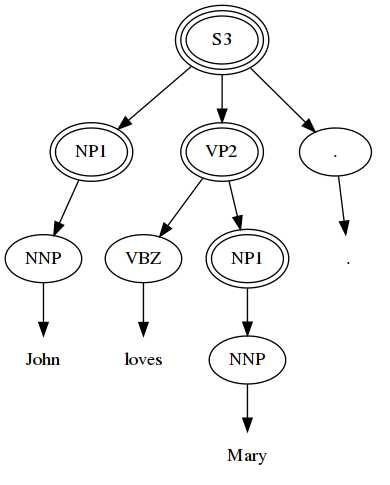
\includegraphics[scale=0.5]{figures/dots/example1.png}
\caption{~\ref{sec:example1}-ben leírt IRTG által generált levezetési fa a \textit{John Loves Mary.} mondat TT-jére.}
\label{fig:example1}
\end{figure}

\begin{figure}[h]
\begin{verbatim}
@(
	S3( *, VP2( VBZ( loves ),  NP1( NNP( Mary ) ) ), .( . ) ), 
	NP1( NNP( John ) ) 
)
\end{verbatim}
\caption{~\ref{sec:example1}-ben leírt IRTG tree interpretációjának kimenete \textit{John Loves Mary.} mondat TT-jére.}
\label{cod:example1output}
\end{figure}



%----------------------------------------------------------------------------
\section{Példa 2}
\label{sec:example2}
%----------------------------------------------------------------------------

\begin{figure}[h]
\begin{verbatim}
\begin{verbatim}
S! -> NP( DT, JJ, NN )
[tree] NP3(?1,?2,?3)

DT -> the_DT
[tree] DT(the)

JJ -> black_JJ
[tree] NN(black)

VB -> cat_VB
[tree] VB(cat)
\end{verbatim}
\caption{Egyszerű három bemenetű IRTG a \textit{the black cat} szószerkezet TT-jének generálására}
\label{cod:example2}
\end{figure}

\begin{figure}[h]
\centering
\graphicspath{./}
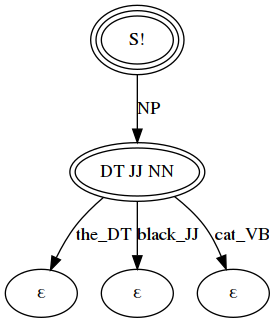
\includegraphics[scale=0.5]{figures/dots/example2.png}
\caption{~\ref{sec:example2}-ben leírt IRTG által generált levezetési fa a \textit{the black cat} szószerkezet TT-jére.}
\label{fig:example2}
\end{figure}

\begin{figure}[h]
\begin{verbatim}
NP3( DT( the ), JJ( black ), NN( cat ) )
\end{verbatim}
\caption{~\ref{sec:example2}-ben leírt IRTG tree interpretációjának kimenete \textit{the black cat} szószerkezet TT-jére. A kimenet maga a  \textit{the black cat} szószerkezet TT-je. }
\label{cod:example2output}
\end{figure}




%----------------------------------------------------------------------------
\section{Példa 3}
\label{sec:example3}
%----------------------------------------------------------------------------

\begin{figure}[h]
\begin{verbatim}
S! -> NP_DT_NP_BAR( DT, NP_BAR)
[tree] @(?2,?1)

NP_BAR -> NP_BAR_JJ_NN(JJ,NN)
[tree] NP3(*,?1,?2)

DT -> the_DT
[tree] DT(the)

JJ -> black_JJ
[tree] NN(black)

VB -> cat_VB
[tree] VB(cat)
\end{verbatim}
\caption{Egyszerű IRTG a \textit{the black cat} szószerkezet TT-jének generálására}
\label{cod:example3}
\end{figure}

\begin{figure}[h]
\centering
\graphicspath{./}
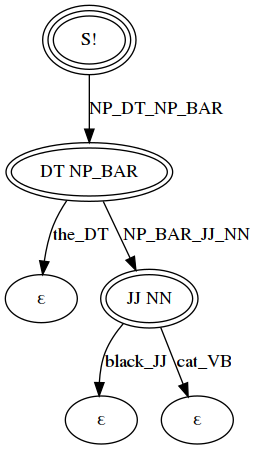
\includegraphics[scale=0.5]{figures/dots/example3.png}
\caption{~\ref{sec:example3}-ban leírt IRTG által generált levezetési fa a \textit{the black cat} szószerkezet TT-jére.}
\label{fig:example3}
\end{figure}

\begin{figure}[h]
\begin{verbatim}
@(  NP3( *, JJ( black ), NN( cat ) ), DT( the ) )
\end{verbatim}
\caption{~\ref{sec:example3}-ben leírt IRTG tree interpretációjának kimenete \textit{the black cat} szószerkezet TT-jére.}
\label{cod:example3output}
\end{figure}




%----------------------------------------------------------------------------
\section{Példa 4}
\label{sec:example4}
%----------------------------------------------------------------------------

\begin{figure}[h]
\begin{verbatim}
S! -> NP_DT_NP_BAR( DT, NP_BAR)
[tree] @(?2,?1)

NP_BAR -> NP_BAR_JJ_NP_BAR(JJ,NP_BAR)
[tree] @(?2,?1)

NP_BAR -> NP_BAR_JJ_NN(JJ,NN)
[tree] NP4(* ,* ,?1 ,?2)

DT -> this_DT
[tree] DT(this)

JJ -> British_JJ
[tree] JJ(British)

JJ -> indastrial_JJ
[tree] JJ(indastrial)

NN -> conglomerate_NN
[tree] NN(conglomerate)
\end{verbatim}
\caption{Egyszerű IRTG a \textit{this British indastrial conglomerate} szószerkezet TT-jének generálására}
\label{cod:example4}
\end{figure}

\begin{figure}[h]
\centering
\graphicspath{./}
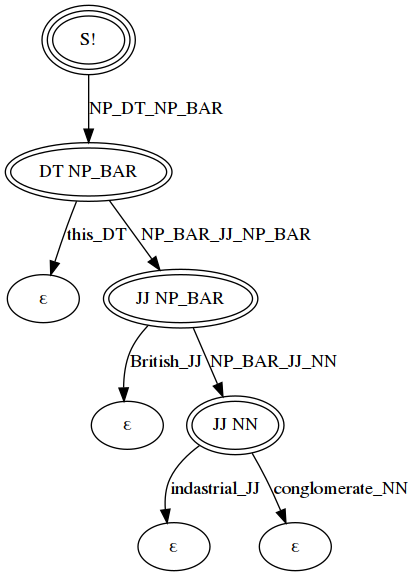
\includegraphics[scale=0.5]{figures/dots/example4.png}
\caption{~\ref{sec:example4}-ben leírt IRTG által generált levezetési fa a \textit{this British indastrial conglomerate} szószerkezet TT-jére.}
\label{fig:example4}
\end{figure}




%----------------------------------------------------------------------------
\section{Példa 5}
\label{sec:example5}
%----------------------------------------------------------------------------

\begin{figure}[h]
\begin{verbatim}
S! -> root_nsubj_NP_S_BAR(NP, S_BAR)
[ud] merge(
			f_dep(merge("(Root/Root :root r<root> :nsubj (d<dep>))", r_dep(?1))),
	 		?2
	 		)

S_BAR -> S_BAR_VP_PUNCT(VP, PUNCT)
[ud] ?1

VP -> dobj_VB_NP(VB,NP)
[ud] merge(f_dep(merge("(r<root> :dobj (d<dep>))", r_dep(?2))),?1)

NP -> NP_NN(NN)
[ud] ?1


NN -> John_NNP
[ud] "(John<root> / John)"

NN -> Mary_NNP
[ud] "(Mary<root> / Mary)"

VB -> loves_VBZ
[ud] "(loves<root> / loves)"

PUNCT -> punct_PUNCT
[ud] "(punct<root> / punct)"
\end{verbatim}
\caption{Egyszerű IRTG a \textit{John Loves Mary.} mondat ud gráfjánek generálására}
\label{cod:example5}
\end{figure}

\begin{figure}[h]
\centering
\graphicspath{./}
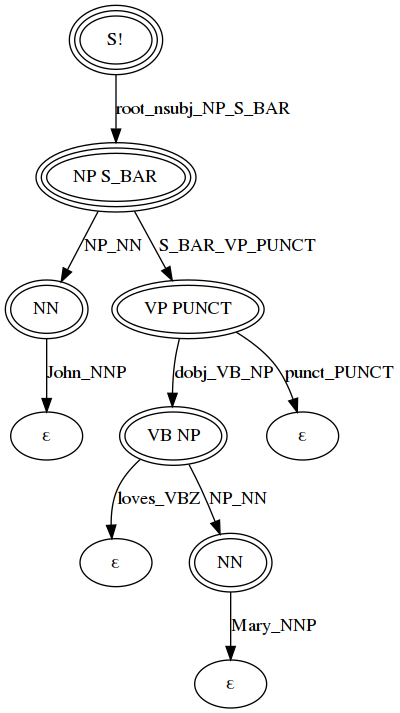
\includegraphics[scale=0.5]{figures/dots/example5_1.png}
\caption{~\ref{sec:example5}-ben leírt IRTG által generált levezetési fa a \textit{John loves Mary.} szószerkezet ud-jét leíró s-graph-ra}
\label{fig:example5.1}
\end{figure}

\begin{figure}[h]
\begin{verbatim}
merge(
	f_dep( merge(
		"(Root/Root :root r<root> :nsubj (d<dep>))",
 		r_dep( "(John<root> / John)" )
		) ),
	 merge(
		f_dep( merge(
					"(r<root> :dobj (d<dep>))", 
					r_dep( "(Mary<root> / Mary)" )
					) ),
 		“(loves<root> / loves)”
		)
	)
\end{verbatim}
\caption{~\ref{sec:example5} ud interpretációjának kimenete}
\label{fig:example5ud}
\end{figure}

\begin{figure}[h]
\centering
\graphicspath{./}
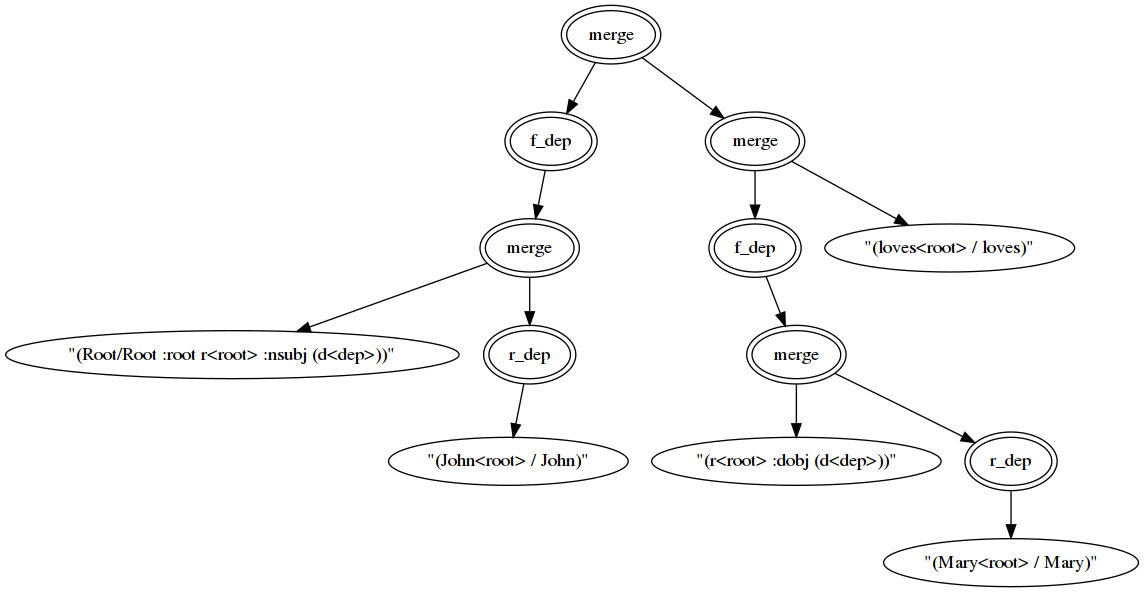
\includegraphics[scale=0.4]{figures/dots/example5_2.png}
\caption{~\ref{sec:example5}-ben leírt IRTG ud interpretációja által generált s-graph kifejezés műveleti fája}
\label{fig:example5.2}
\end{figure}

"(Root/Root :root loves<root>/loves :nsubj (John/John) :dobj (Mary/Mary))"
\begin{figure}[h]
\centering
\graphicspath{./}
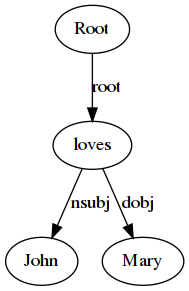
\includegraphics[scale=0.5]{figures/dots/example5_3.png}
\caption{~\ref{sec:example5}-ben leírt IRTG ud interpretációja által generált s-graph kifejezés végeredménye}
\label{fig:example5.3}
\end{figure}




%----------------------------------------------------------------------------
\section{Példa 6}
\label{sec:example6}
%----------------------------------------------------------------------------

\begin{figure}[h]
\begin{verbatim}
S! -> root_nsubj_NP_S_BAR(NP, S_BAR)
[tree] @(?2,?1)
[ud] merge(
			f_dep(merge("(Root/Root :root r<root> :nsubj (d<dep>))", r_dep(?1))),
			?2
			)
[fourlang] merge(
				f_dep(merge("(Root/Root :root r<root> :1,0 (d<dep>))", r_dep(?1))),
				?2
				)

S_BAR -> S_NP_VP(VP, PUNCT)
[tree] S3( *, ?1, ?2)
[ud] ?1
[fourlang] ?1

VP -> dobj_VB_NP(VB,NP)
[tree] VP2(?1,?2)
[ud] merge(
			f_dep(merge("(r<root> :dobj (d<dep>))", r_dep(?2))),
			?1
			)
[fourlang] merge(
				f_dep(merge("(r<root> :2 (d<dep>))", r_dep(?2))),
				?1
				)

NP -> NP_NN(NN)
[tree] NP1(?1)
[ud] ?1
[fourlang] ?1


NN -> John_NNP
[tree] NNP(John)
[ud] "(John<root> / John)"
[fourlang] "(John<root> / John)"

NN -> Mary_NNP
[tree] NNP(Mary)
[ud] "(Mary<root> / Mary)"
[fourlang] "(Mary<root> / Mary)"

VB -> loves_VBZ
[tree] VBZ(loves)
[ud] "(loves<root> / loves)"
[fourlang] "(loves<root> / loves)"

PUNCT -> punct_PUNCT
[tree] .(.)
[ud] "(punct<root> / punct)"
[fourlang] "(punct<root> / punct)"
\end{verbatim}
\caption{IRTG három algebrával a \textit{John Loves Mary.} mondat szintaktikai fájának, ud gráfjának és 4lang gráfjának generálására}
\label{cod:example6}
\end{figure}

\begin{figure}[h]
\centering
\graphicspath{./}
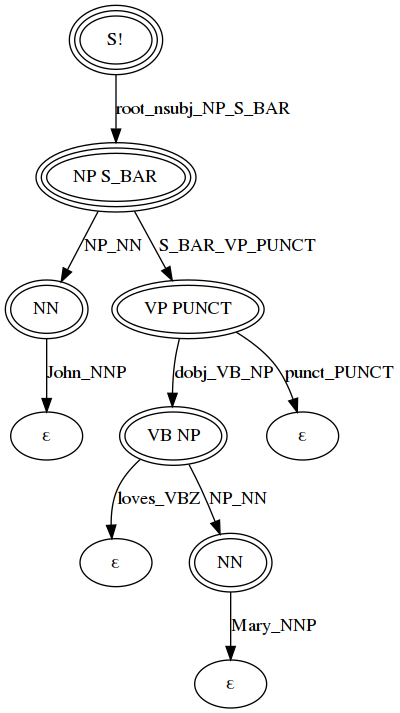
\includegraphics[scale=0.5]{figures/dots/example6_1.png}
\caption{~\ref{sec:example6}-ban leírt IRTG által generált levezetési fa a \textit{John loves Mary.} szószerkezet 4lang-ját leíró s-graph-ra}
\label{fig:example6}
\end{figure}

\begin{figure}[h]
\begin{verbatim}
merge(
	f_dep( 
		merge(
			"(Root/Root :root r<root> :1,0 (d<dep>))",
 			r_dep( 
				"(John<root> / John)" 
				)
			) 
		),
 		merge(
			f_dep( 
					merge(
						"(r<root> :2 (d<dep>))", 
						r_dep( 
							"(Mary<root> / Mary)" 	
							)
						) 
				),
			 “(loves<root> / loves)”
			)
)
\end{verbatim}
\caption{~\ref{sec:example6} fourlang interpretációjának kimenete}
\label{fig:example6fourlang}
\end{figure}

\begin{figure}[h]
\centering
\graphicspath{./}
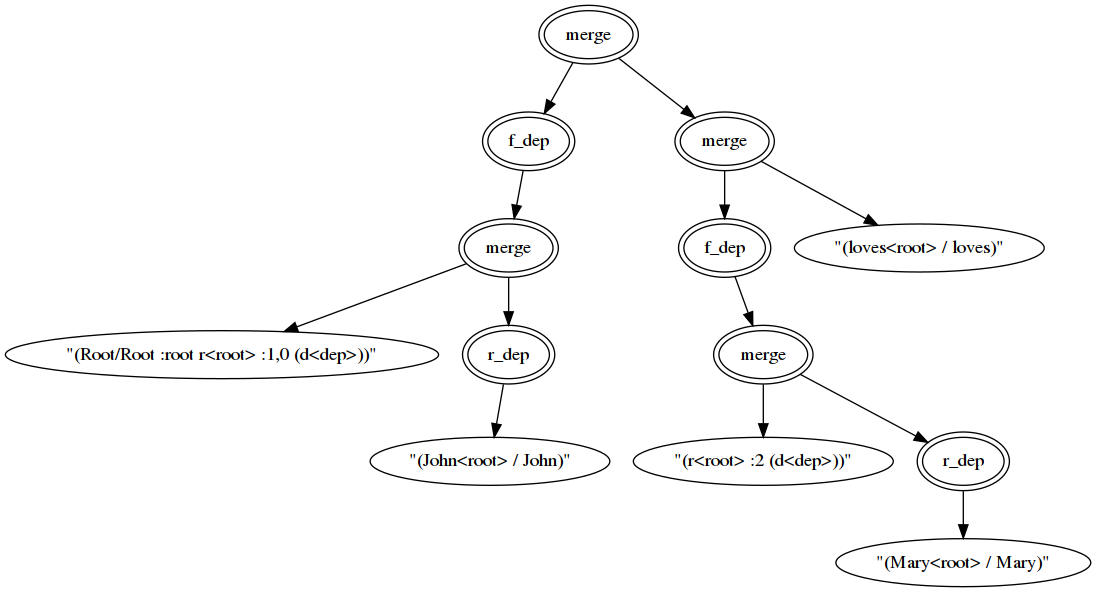
\includegraphics[scale=0.4]{figures/dots/example6_2.png}
\caption{~\ref{sec:example6}-ben leírt IRTG fourlang interpretációja által generált s-graph kifejezés műveleti fája}
\label{fig:example6.2}
\end{figure}

\begin{figure}[h]
\centering
\graphicspath{./}
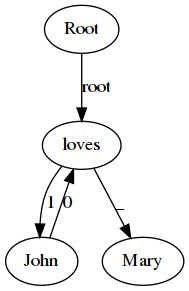
\includegraphics[scale=0.5]{figures/dots/example6_3.png}
\caption{~\ref{sec:example6}-ben leírt IRTG fourlang interpretációja által generált s-graph kifejezés végeredménye}
\label{fig:example6.3}
\end{figure}




%----------------------------------------------------------------------------
\section{Példa 7}
\label{sec:example7}
%----------------------------------------------------------------------------

\begin{figure}[h]
\begin{verbatim}
//merge start
@(																				
	//merge start
	@(																			
		//graph1
		"( [ Root | | Root ] <root- ( [ r | root ] <nsubj- [ d | dep ] ) )",	
		//graph2
	 	"( [ John | root | John ] )",
	 	//tag of graph1
		dep,							
		//tag of graph2
		root,						
		//tag to forget	
		dep							
	//merge end
	),								
	//merge start
 	@(								
 		//merge start
		@(							
			//graph1
			"([ r | root ] <dobj- [ d | dep ] )", 		
			//graph2	
			"( [ Mary | root | Mary] )",
			//tag of graph1				
			dep,						
			//tag of graph2
			root,					
			//tag to forget	
			dep						
		//merge end
		) ,							
		//graph2
		“( [ loves | root | loves ] )”
	//megre end					
	)								
//merge end
)									
\end{verbatim}
\caption{Példa kód az SGA fejlesztésével kapcsolatos koncepció szemléltetésére.
			A példa a \textit{John loves Mary.} mondat UD-gráfjára adott kimenetet dolgozza fel az új szintaxissal.}
\label{cod:example7}
\end{figure}



%----------------------------------------------------------------------------
\section{Példa 8}
\label{sec:example8}
%----------------------------------------------------------------------------

\begin{verbatim}


//merge the root of the left graph with root of the right graph
( 
//merge the dep of left graph with the root of the right graph, then we forget dep
( "( [ Root | | Root ] <root- ( [ r | root ] <nsubj- [ d | dep ] ) )" 
>dep@root< 
"( [ John | root | John ] )" X dep ) 

>root@root<

//merge the root of the left graph with root of the right graph
( 

//merge the dep of left graph with the root of the right graph, then we forget dep
( "([ r | root ] <dobj- [ d | dep ] )" 
>dep@root< 	//merge on dep of left graph and root of right graph
"( [ Mary | root | Mary ]  )" X	dep ) 

>root@root<	//merge on root of left graph and root of right graph

“( [ loves | root | loves ]  )” )

)
\end{verbatim}



%----------------------------------------------------------------------------
\section{Példa IRTG1}
\label{sec:exampleIRTG1}
%----------------------------------------------------------------------------
\begin{verbatim}
{= 
irtgBase : Temp := 
	{|
		{@e@}{@t@}{$left$} -> {$header$}
		{@e@}{@t@}[string] {$string$}
		{@e@}{@t@}[tree] {$syntax_tree$}
		{@e@}{@t@}[ud] {$ud_graph$}
		{@e@}{@t@}[4lang] {$fourlang_graph$}
	|}
=}
{= 
irtgDataBase : Type  :=  left, header, string, syntax_tree, ud_graph, fourlang_graph : Temp
=}
{= 
irtgData : irtgDataBase  :=  
		left		:={|{$word_class$}|},
		header		:={|{$word$}_{$word_class$}|},
		string		:={|{$word$}|},
		syntax_tree	:={|{$word_class$}({$word$})|},
		ud_graph	:={|"({$word$}<root>\{$word$})"|},
		fourlang_graph	:={|"({$concept$}<root>\{$concept$})"|}
=}
{= 
termBase : Temp  :=  {+ irtgBase :+ irtgData +}
=}
{= 
termDataBase : Type  :=  word_class, word, concept : Template
=}
{=data0 :termDataBase  := word_class := {"NN"}, word := {"dog"}, concept := {"dog"} =}
{=data1 :termDataBase  := word_class := {"NN"}, word := {"cat"}, concept := {"cat"} =}
{=data2 :termDataBase  := word_class := {"NN"}, word := {"fish"}, concept := {"fish"} =}
{=data3 :termDataBase  := word_class := {"NN"}, word := {"mouse"}, concept := {"mouse"} =}
{=data4 :termDataBase  := word_class := {"NN"}, word := {"lion"}, concept := {"lion"} =}
{=data5 :termDataBase  := word_class := {"NN"}, word := {"monkey"}, concept := {"monkey"} =}
{=data6 :termDataBase  := word_class := {"NN"}, word := {"fox"}, concept := {"fox"} =}
{=data7 :termDataBase  := word_class := {"NN"}, word := {"bird"}, concept := {"bird"} =}
{=data8 :termDataBase  := word_class := {"NN"}, word := {"tiger"}, concept := {"tiger"} =}
{=data9 :termDataBase  := word_class := {"NN"}, word := {"owl"}, concept := {"owl"} =}
{* 
	{+ 
	termBase.copy :+ data0 : 
		left.cont.word_class 		:+ word_class,
		header.cont.word 		:+ word,
		header.cont.word_class 		:+ word_class,
		string.cont.word	 	:+ word,
		syntax_tree.cont.word_class	:+ word_class,
		syntax_tree.cont.word 		:+ word,
		ud_graph.cont.word.0		:+ word,
		ud_graph.cont.word.1		:+ word,
		fourlang_graph.cont.concept.0	:+ concept,
		fourlang_graph.cont.concept.1	:+ concept
	+}
*}
{@e@}
{* 
	{+ 
	termBase.copy :+ data1 : 
		left.cont.word_class 		:+ word_class,
		header.cont.word 		:+ word,
		header.cont.word_class 		:+ word_class,
		string.cont.word	 	:+ word,
		syntax_tree.cont.word_class	:+ word_class,
		syntax_tree.cont.word 		:+ word,
		ud_graph.cont.word.0		:+ word,
		ud_graph.cont.word.1		:+ word,
		fourlang_graph.cont.concept.0	:+ concept,
		fourlang_graph.cont.concept.1	:+ concept
	+}
*}
{@e@}
{* 
	{+ 
	termBase.copy :+ data2 : 
		left.cont.word_class 		:+ word_class,
		header.cont.word 		:+ word,
		header.cont.word_class 		:+ word_class,
		string.cont.word	 	:+ word,
		syntax_tree.cont.word_class	:+ word_class,
		syntax_tree.cont.word 		:+ word,
		ud_graph.cont.word.0		:+ word,
		ud_graph.cont.word.1		:+ word,
		fourlang_graph.cont.concept.0	:+ concept,
		fourlang_graph.cont.concept.1	:+ concept
	+}
*}
{@e@}
{* 
	{+ 
	termBase.copy :+ data3 : 
		left.cont.word_class 		:+ word_class,
		header.cont.word 		:+ word,
		header.cont.word_class 		:+ word_class,
		string.cont.word	 	:+ word,
		syntax_tree.cont.word_class	:+ word_class,
		syntax_tree.cont.word 		:+ word,
		ud_graph.cont.word.0		:+ word,
		ud_graph.cont.word.1		:+ word,
		fourlang_graph.cont.concept.0	:+ concept,
		fourlang_graph.cont.concept.1	:+ concept
	+}
*}
{@e@}
{* 
	{+ 
	termBase.copy :+ data4 : 
		left.cont.word_class 		:+ word_class,
		header.cont.word 		:+ word,
		header.cont.word_class 		:+ word_class,
		string.cont.word	 	:+ word,
		syntax_tree.cont.word_class	:+ word_class,
		syntax_tree.cont.word 		:+ word,
		ud_graph.cont.word.0		:+ word,
		ud_graph.cont.word.1		:+ word,
		fourlang_graph.cont.concept.0	:+ concept,
		fourlang_graph.cont.concept.1	:+ concept
	+}
*}
{@e@}
{* 
	{+ 
	termBase.copy :+ data5 : 
		left.cont.word_class 		:+ word_class,
		header.cont.word 		:+ word,
		header.cont.word_class 		:+ word_class,
		string.cont.word	 	:+ word,
		syntax_tree.cont.word_class	:+ word_class,
		syntax_tree.cont.word 		:+ word,
		ud_graph.cont.word.0		:+ word,
		ud_graph.cont.word.1		:+ word,
		fourlang_graph.cont.concept.0	:+ concept,
		fourlang_graph.cont.concept.1	:+ concept
	+}
*}
{@e@}
{* 
	{+ 
	termBase.copy :+ data6 : 
		left.cont.word_class 		:+ word_class,
		header.cont.word 		:+ word,
		header.cont.word_class 		:+ word_class,
		string.cont.word	 	:+ word,
		syntax_tree.cont.word_class	:+ word_class,
		syntax_tree.cont.word 		:+ word,
		ud_graph.cont.word.0		:+ word,
		ud_graph.cont.word.1		:+ word,
		fourlang_graph.cont.concept.0	:+ concept,
		fourlang_graph.cont.concept.1	:+ concept
	+}
*}
{@e@}
{* 
	{+ 
	termBase.copy :+ data7 : 
		left.cont.word_class 		:+ word_class,
		header.cont.word 		:+ word,
		header.cont.word_class 		:+ word_class,
		string.cont.word	 	:+ word,
		syntax_tree.cont.word_class	:+ word_class,
		syntax_tree.cont.word 		:+ word,
		ud_graph.cont.word.0		:+ word,
		ud_graph.cont.word.1		:+ word,
		fourlang_graph.cont.concept.0	:+ concept,
		fourlang_graph.cont.concept.1	:+ concept
	+}
*}
{@e@}
{* 
	{+ 
	termBase.copy :+ data8 : 
		left.cont.word_class 		:+ word_class,
		header.cont.word 		:+ word,
		header.cont.word_class 		:+ word_class,
		string.cont.word	 	:+ word,
		syntax_tree.cont.word_class	:+ word_class,
		syntax_tree.cont.word 		:+ word,
		ud_graph.cont.word.0		:+ word,
		ud_graph.cont.word.1		:+ word,
		fourlang_graph.cont.concept.0	:+ concept,
		fourlang_graph.cont.concept.1	:+ concept
	+}
*}
{@e@}
{* 
	{+ 
	termBase.copy :+ data9 : 
		left.cont.word_class 		:+ word_class,
		header.cont.word 		:+ word,
		header.cont.word_class 		:+ word_class,
		string.cont.word	 	:+ word,
		syntax_tree.cont.word_class	:+ word_class,
		syntax_tree.cont.word 		:+ word,
		ud_graph.cont.word.0		:+ word,
		ud_graph.cont.word.1		:+ word,
		fourlang_graph.cont.concept.0	:+ concept,
		fourlang_graph.cont.concept.1	:+ concept
	+}
*}
{@e@}
\end{verbatim}


%----------------------------------------------------------------------------
\section{Példa IRTG2}
\label{sec:exampleIRTG2}
%----------------------------------------------------------------------------
\begin{verbatim}
{= 
dataFile :File := {"/home/boss/Documents/Git/SlimeAnUTLE/test_codes/irtg_example2data"};
result :List:Temp := {+ dataFile.termBase :+ dataFile.datas +} 
=}
{*
{+ 
result :+ dataFile.datas : 
	0.slots.iter:+0, 
	1.slots.iter:+1, 
	2.slots.iter:+2, 
	3.slots.iter:+3, 
	4.slots.iter:+4, 
	5.slots.iter:+5, 
	6.slots.iter:+6, 
	7.slots.iter:+7, 
	8.slots.iter:+8, 
	9.slots.iter:+9 
+}: {@e@} 
*}

\end{verbatim}

\begin{verbatim}
{# Data for example 2 #}
{= 
irtgBase : Temp := 
	{|
		{@e;t@}{$left$} -> {$header$}
		{@e;t@}[string] {$string$}
		{@e;t@}[tree] {$syntax_tree$}
		{@e;t@}[ud] {$ud_graph$}
		{@e;t@}[4lang] {$fourlang_graph$}
	|};

irtgDataBase : Type  :=  left, header, string, syntax_tree, ud_graph, fourlang_graph : Temp;

irtgData : irtgDataBase  :=  
	{|
		{$word_class$};{$word$}_{$word_class$};
		{$word$};
		{$word_class$}({$word$});
		"({$word$}<root>\{$word$})";
		"({$concept$}<root>\{$concept$})"
	|};

termBase : Temp  :=  {+ irtgBase :+ irtgData +};

termDataBase : Type  :=  word_class, word, concept : Template;

datas :List:termDataBase :=
	{= :termDataBase  := 	{"NN"}, {"dog"},   {"dog"} 	=},
	{= :termDataBase  := 	{"NN"}, {"cat"},   {"cat"} 	=},
	{= :termDataBase  := 	{"NN"}, {"fish"},  {"fish"} 	=},
	{= :termDataBase  := 	{"NN"}, {"mouse"}, {"mouse"} 	=},
	{= :termDataBase  :=	{"NN"}, {"lion"},  {"lion"} 	=},
	{= :termDataBase  := 	{"NN"}, {"monkey"},{"monkey"} 	=},
	{= :termDataBase  := 	{"NN"}, {"fox"},   {"fox"} 	=},
	{= :termDataBase  := 	{"NN"}, {"bird"},  {"bird"} 	=},
	{= :termDataBase  := 	{"NN"}, {"tiger"}, {"tiger"} 	=},
	{= :termDataBase  := 	{"NN"}, {"owl"},   {"owl"} 	=}
=}

\end{verbatim}

%----------------------------------------------------------------------------
\section{Példa IRTG3}
\label{sec:exampleIRTG3}
%----------------------------------------------------------------------------
\begin{verbatim}
{= 
irtgBase,IB : Temp := 
	{|
		<@e;t <$left  -> [$header
		<@e;t [string] [$string
		<@e;t [tree] [$syntax_tree
		<@e;t [ud] [$ud_graph
		<@e;t [4lang] [$fourlang_graph
	|}

IDB,irtgDataBase : Type  :=  left, header, string, syntax_tree, ud_graph, fourlang_graph : Template

irtgData,ID : IDB  :=  
	{|
		<$word_class ;<$word _<$word_class ;
		<$word ;
		<$word_class (<$word );
		"(<$word <root>\<$word )";
		"(<$concept <root>\<$concept )"
	|}

termBase,TB : Temp  :=  <+IB:+ID

TDB,termDataBase : Type  :=  word_class, word, concept : Temp

datas,D :List:TDB :=
	 [=:TDB:= [|NN;dog;dog 
	,[=:TDB:= [|NN;cat;cat 
	,[=:TDB:= [|NN;owl;owl 
	,[=:TDB:= [|NN;fox;fox 
	,[=:TDB:= [|NN;fish;fish 
	,[=:TDB:= [|NN;lion;lion 
	,[=:TDB:= [|NN;bird;bird 
	,[=:TDB:= [|NN;mouse;mouse 
	,[=:TDB:= [|NN;tiger;tiger 
	,[=:TDB:= [|NN;monkey;monkey 

result,R :List:Temp := <+TB:+D 
=}
<*{+ 
R :+ D : 
	0.slots.iter:+0, 
	1.slots.iter:+1, 
	2.slots.iter:+2, 
	3.slots.iter:+3, 
	4.slots.iter:+4, 
	5.slots.iter:+5, 
	6.slots.iter:+6, 
	7.slots.iter:+7, 
	8.slots.iter:+8, 
	9.slots.iter:+9 
+}:<@e

\end{verbatim}


%----------------------------------------------------------------------------
\section{Példa IRTG4}
\label{sec:exampleIRTG4}
%----------------------------------------------------------------------------
\begin{verbatim}
{= 
irtgBase,IB : Temp := 
	{|
		<@e;t //[$comm
		<@e;t <$left  -> [$header
		<@e;t [string] [$string
		<@e;t [tree] [$tree
		<@e;t [ud] [$ud
		<@e;t [4lang] [$four
	|}

IDB,irtgDataBase : Type  :=  comm, left, header, string, tree, ud, four : Temp

irtgData1,ID1 : IDB  :=  
	{|
		{$comm$};
		NP;_NP2_{$edge_ud$}_{$arg1$}_{$arg2$}({$arg1$}, {$arg2$}); 
        	*(?1, ?2);
		NP2(?1,?2); 
		merge(f_dep(merge("(r<root> :{$edge_ud$} (d<dep>))",r_dep(?1))),?2);
		merge(f_dep(merge("(r<root> :{$edge_4lang$}) (d<dep>))",r_dep(?1))),?2)
	|}

irtgData2,ID2 : IDB  := ID1.0, ID1.1, ID1.2, ID1.3, ID1.4, ID1.5,
	{|?2|}
	

irtgData3,ID3 : IDB  := ID1.0, ID1.1, ID1.2, ID1.3, ID1.4, ID1.5,
	{|f_dep(merge(merge(?1, "(HAS / HAS :1 (d<dep>) :2 (r<root>))"), r_dep(?2)))|}

nounPhraseBase1,NPB1 : Temp  :=  <+IB.copy:+ID1
nounPhraseBase1,NPB2 : Temp  :=  <+IB.copy:+ID2
nounPhraseBase1,NPB3 : Temp  :=  <+IB.copy:+ID3

NPDB,nounPhraseDataBase : Type  :=  comm,  arg1, arg2, edge_ud, edge_4lang : Text

datas1,D1 :List:NPDB :=
	 [=:NPDB:= {"cute cat"}			,{"JJ"}	,{"NN"}		,{"amod"}	,{"0"}
	,[=:NPDB:= {"electricity charges"}	,{"NN"}	,{"NNS"}	,{"compound"}	,{"0_compound_nouns"}
	,[=:NPDB:= {"car safety"}		,{"NN"}	,{"NN"}		,{"compound"}	,{"0_compound_nouns"}
	,[=:NPDB:= {"one dog"}			,{"CD"}	,{"NN"}		,{"nummod"}	,{"0"}
	,[=:NPDB:= {"three dogs"}		,{"CD"}	,{"NNS"}	,{"nummod"}	,{"0"}
	,[=:NPDB:= {"cute cats"}		,{"JJ"}	,{"NNS"}	,{"amod"}	,{"0"}
	,[=:NPDB:= {"John Smith"}		,{"NNP"},{"NNP"}	,{"flat"}	,{"0_flat_name"}
	
datas2,D2 :List:NPDB :=
	 [=:NPDB:= {"the Examiner"}	,{"DT"}	,{"NNP"}	,{"det"}
	,[=:NPDB:= {"a cat"}		,{"DT"}	,{"NN"}		,{"det"}
	,[=:NPDB:= {"the cats"}		,{"DT"}	,{"NNS"}	,{"det"}
	
datas3,D3 :List:NPDB :=
	 [=:NPDB:= {"my cat"}		,{"PRPDOLLAR"}	,{"NN"}		,{"nmod:poss"}
	,[=:NPDB:= {"my cats"}		,{"PRPDOLLAR"}	,{"NNS"}	,{"nmod:poss"}

result1,R1 :List:Temp := <+NPB1:+D1
result2,R2 :List:Temp := <+NPB2:+D2
result3,R3 :List:Temp := <+NPB3:+D3
=}
<*{+ 
R1 :+ D1 : 
	0.slots.iter:+0, 
	1.slots.iter:+1, 
	2.slots.iter:+2, 
	3.slots.iter:+3, 
	4.slots.iter:+4, 
	5.slots.iter:+5, 
	6.slots.iter:+6
R2 :+ D2 : 
	0.slots.iter:+0, 
	1.slots.iter:+1, 
	2.slots.iter:+2
R3 :+ D3 : 
	0.slots.iter:+0, 
	1.slots.iter:+1
+}:<@e 

\end{verbatim}


%----------------------------------------------------------------------------
\section{Példa ANTLR}
\label{sec:exampleANTLR}
%----------------------------------------------------------------------------

\begin{verbatim}
{=
shortRuleBase, SRB	:Temp := {|<$typeB _<$typeM  : '<$pattB;pattM ' -> 
					pushMode(<$modeB _<$modeM )<@sc <$wrap |}
longRuleBase, LRB    	:Temp := {|<$typeB _<$typeM _<$fromB _<$fromM  : '<$pattB;pattM ' ->
					type(<$typeB _<$typeM ), pushMode(<$modeB _<$modeM )<@sc <$wrap |}

BDB,bracDataBase : Type := typeB, pattB, modeB :Temp
bracDatas,BD :List:BDB :=
	 [=:BDB:= [|BOB;{;B
	,[=:BDB:= [|OLB;[;O
	,[=:BDB:= [|COB;<;C

MDB,modeDataBase : Type := typeM, pattM, modeM, wrap :Temp
modeDatas3,MD3 :List:MDB :=
	 [=:MDB:= [|SLOT;$;SLSP;<@e 
	,[=:MDB:= [|SPEC;@;SLSP;<@e 
	,[=:MDB:= [|TEXT;";TEXT;<@e;e 
modeDatas9,MD9 :List:MDB := MD3.0, MD3.1
	,[=:MDB:= [|REFE;&;REFE;<@e 
	,[=:MDB:= [|EXTE;*;OPER;<@e 
	,[=:MDB:= [|PLUS;+;OPER;<@e 
	,[=:MDB:= [|DECL;=;OPER;<@e 
	,[=:MDB:= [|DELE;X;OPER;<@e 
	,[=:MDB:= [|TEXT;";TEXT;<@e 
	,[=:MDB:= [|TEMP;|;TEMP;<@e;e 
fromBData ,FBD	:List:Temp := [|B;O;C
fromMData ,FMD	:List:Temp := [|O;T
=}

{=
datasBasic, DB	: List:Temp := [+SRB:+BD

dataBasicBloc, DBB	:List:Temp := [+ DB.0 :+ MD9
dataBasicOnel, DBO	:List:Temp := [+ DB.1 :+ MD9
dataBasicComp, DBC	:List:Temp := [+ DB.2 :+ MD9
=}
{*
{&List:Temp:&DB[BOC]&}
{@e@}
*}

{=
datasLong, DL		: List:Temp := [+ LRB.fromM :+ FMD
DLOper, DLO	: List:Temp := [+ DL.0.fromB :+ FBD
DLTemp, DLT	: List:Temp := [+ DL.1.fromB :+ FBD

DLBlocOper, DLBO: List:Temp := [+ DLO.0 :+ BD
DLOnelOper, DLOO: List:Temp := [+ DLO.1 :+ BD
DLCompOper, DLCO: List:Temp := [+ DLO.2 :+ BD
DLBlocTemp, DLBT: List:Temp := [+ DLT.0 :+ BD
DLOnelTemp, DLOT: List:Temp := [+ DLT.1 :+ BD
DLCompTemp, DLCT: List:Temp := [+ DLT.2 :+ BD
 
DLBOBloc, DLBOB: List:Temp := [+ DLBO.0 :+ MD9
DLBOOnel, DLBOO: List:Temp := [+ DLBO.1 :+ MD9
DLBOComp, DLBOC: List:Temp := [+ DLBO.2 :+ MD9
DLOOBloc, DLOOB: List:Temp := [+ DLOO.0 :+ MD9
DLOOOnel, DLOOO: List:Temp := [+ DLOO.1 :+ MD9
DLOOComp, DLOOC: List:Temp := [+ DLOO.2 :+ MD9
DLCOBloc, DLCOB: List:Temp := [+ DLCO.0 :+ MD9
DLCOOnel, DLCOO: List:Temp := [+ DLCO.1 :+ MD9
DLCOComp, DLCOC: List:Temp := [+ DLCO.2 :+ MD9
DLBTBloc, DLBTB: List:Temp := [+ DLBT.0 :+ MD3
DLBTOnel, DLBTO: List:Temp := [+ DLBT.1 :+ MD3
DLBTComp, DLBTC: List:Temp := [+ DLBT.2 :+ MD3
DLOTBloc, DLOTB: List:Temp := [+ DLOT.0 :+ MD3
DLOTOnel, DLOTO: List:Temp := [+ DLOT.1 :+ MD3
DLOTComp, DLOTC: List:Temp := [+ DLOT.2 :+ MD3
DLCTBloc, DLCTB: List:Temp := [+ DLCT.0 :+ MD3
DLCTOnel, DLCTO: List:Temp := [+ DLCT.1 :+ MD3
DLCTComp, DLCTC: List:Temp := [+ DLCT.2 :+ MD3
=}

{*
	{&List:Temp:&DLBO[BOC]&}{@e@}
	{&List:Temp:&DLOO[BOC]&}{@e@}
	{&List:Temp:&DLCO[BOC]&}{@e@}
	{@e@}
	{&List:Temp:&DLBT[BOC]&}{@e@}
	{&List:Temp:&DLOT[BOC]&}{@e@}
	{&List:Temp:&DLCT[BOC]&}{@e@}
*}


\end{verbatim}

Ilyen kimenetet ad:

\begin{verbatim}
BOB_SLOT : '{$' -> pushMode(B_SLSP);
BOB_SPEC : '{@' -> pushMode(B_SLSP);
BOB_REFE : '{&' -> pushMode(B_REFE);
BOB_EXTE : '{*' -> pushMode(B_OPER);
BOB_PLUS : '{+' -> pushMode(B_OPER);
BOB_DECL : '{=' -> pushMode(B_OPER);
BOB_DELE : '{X' -> pushMode(B_OPER);
BOB_TEXT : '{"' -> pushMode(B_TEXT);
BOB_TEMP : '{|' -> pushMode(B_TEMP);

OLB_SLOT : '[$' -> pushMode(O_SLSP);
OLB_SPEC : '[@' -> pushMode(O_SLSP);
OLB_REFE : '[&' -> pushMode(O_REFE);
OLB_EXTE : '[*' -> pushMode(O_OPER);
OLB_PLUS : '[+' -> pushMode(O_OPER);
OLB_DECL : '[=' -> pushMode(O_OPER);
OLB_DELE : '[X' -> pushMode(O_OPER);
OLB_TEXT : '["' -> pushMode(O_TEXT);
OLB_TEMP : '[|' -> pushMode(O_TEMP);

COB_SLOT : '<$' -> pushMode(C_SLSP);
COB_SPEC : '<@' -> pushMode(C_SLSP);
COB_REFE : '<&' -> pushMode(C_REFE);
COB_EXTE : '<*' -> pushMode(C_OPER);
COB_PLUS : '<+' -> pushMode(C_OPER);
COB_DECL : '<=' -> pushMode(C_OPER);
COB_DELE : '<X' -> pushMode(C_OPER);
COB_TEXT : '<"' -> pushMode(C_TEXT);
COB_TEMP : '<|' -> pushMode(C_TEMP);


BOB_SLOT_B_O : '{$' -> type(BOB_SLOT), pushMode(B_SLSP);
BOB_SPEC_B_O : '{@' -> type(BOB_SPEC), pushMode(B_SLSP);
BOB_REFE_B_O : '{&' -> type(BOB_REFE), pushMode(B_REFE);
BOB_EXTE_B_O : '{*' -> type(BOB_EXTE), pushMode(B_OPER);
BOB_PLUS_B_O : '{+' -> type(BOB_PLUS), pushMode(B_OPER);
BOB_DECL_B_O : '{=' -> type(BOB_DECL), pushMode(B_OPER);
BOB_DELE_B_O : '{X' -> type(BOB_DELE), pushMode(B_OPER);
BOB_TEXT_B_O : '{"' -> type(BOB_TEXT), pushMode(B_TEXT);
BOB_TEMP_B_O : '{|' -> type(BOB_TEMP), pushMode(B_TEMP);

OLB_SLOT_B_O : '[$' -> type(OLB_SLOT), pushMode(O_SLSP);
OLB_SPEC_B_O : '[@' -> type(OLB_SPEC), pushMode(O_SLSP);
OLB_REFE_B_O : '[&' -> type(OLB_REFE), pushMode(O_REFE);
OLB_EXTE_B_O : '[*' -> type(OLB_EXTE), pushMode(O_OPER);
OLB_PLUS_B_O : '[+' -> type(OLB_PLUS), pushMode(O_OPER);
OLB_DECL_B_O : '[=' -> type(OLB_DECL), pushMode(O_OPER);
OLB_DELE_B_O : '[X' -> type(OLB_DELE), pushMode(O_OPER);
OLB_TEXT_B_O : '["' -> type(OLB_TEXT), pushMode(O_TEXT);
OLB_TEMP_B_O : '[|' -> type(OLB_TEMP), pushMode(O_TEMP);

COB_SLOT_B_O : '<$' -> type(COB_SLOT), pushMode(C_SLSP);
COB_SPEC_B_O : '<@' -> type(COB_SPEC), pushMode(C_SLSP);
COB_REFE_B_O : '<&' -> type(COB_REFE), pushMode(C_REFE);
COB_EXTE_B_O : '<*' -> type(COB_EXTE), pushMode(C_OPER);
COB_PLUS_B_O : '<+' -> type(COB_PLUS), pushMode(C_OPER);
COB_DECL_B_O : '<=' -> type(COB_DECL), pushMode(C_OPER);
COB_DELE_B_O : '<X' -> type(COB_DELE), pushMode(C_OPER);
COB_TEXT_B_O : '<"' -> type(COB_TEXT), pushMode(C_TEXT);
COB_TEMP_B_O : '<|' -> type(COB_TEMP), pushMode(C_TEMP);


BOB_SLOT_O_O : '{$' -> type(BOB_SLOT), pushMode(B_SLSP);
BOB_SPEC_O_O : '{@' -> type(BOB_SPEC), pushMode(B_SLSP);
BOB_REFE_O_O : '{&' -> type(BOB_REFE), pushMode(B_REFE);
BOB_EXTE_O_O : '{*' -> type(BOB_EXTE), pushMode(B_OPER);
BOB_PLUS_O_O : '{+' -> type(BOB_PLUS), pushMode(B_OPER);
BOB_DECL_O_O : '{=' -> type(BOB_DECL), pushMode(B_OPER);
BOB_DELE_O_O : '{X' -> type(BOB_DELE), pushMode(B_OPER);
BOB_TEXT_O_O : '{"' -> type(BOB_TEXT), pushMode(B_TEXT);
BOB_TEMP_O_O : '{|' -> type(BOB_TEMP), pushMode(B_TEMP);

OLB_SLOT_O_O : '[$' -> type(OLB_SLOT), pushMode(O_SLSP);
OLB_SPEC_O_O : '[@' -> type(OLB_SPEC), pushMode(O_SLSP);
OLB_REFE_O_O : '[&' -> type(OLB_REFE), pushMode(O_REFE);
OLB_EXTE_O_O : '[*' -> type(OLB_EXTE), pushMode(O_OPER);
OLB_PLUS_O_O : '[+' -> type(OLB_PLUS), pushMode(O_OPER);
OLB_DECL_O_O : '[=' -> type(OLB_DECL), pushMode(O_OPER);
OLB_DELE_O_O : '[X' -> type(OLB_DELE), pushMode(O_OPER);
OLB_TEXT_O_O : '["' -> type(OLB_TEXT), pushMode(O_TEXT);
OLB_TEMP_O_O : '[|' -> type(OLB_TEMP), pushMode(O_TEMP);

COB_SLOT_O_O : '<$' -> type(COB_SLOT), pushMode(C_SLSP);
COB_SPEC_O_O : '<@' -> type(COB_SPEC), pushMode(C_SLSP);
COB_REFE_O_O : '<&' -> type(COB_REFE), pushMode(C_REFE);
COB_EXTE_O_O : '<*' -> type(COB_EXTE), pushMode(C_OPER);
COB_PLUS_O_O : '<+' -> type(COB_PLUS), pushMode(C_OPER);
COB_DECL_O_O : '<=' -> type(COB_DECL), pushMode(C_OPER);
COB_DELE_O_O : '<X' -> type(COB_DELE), pushMode(C_OPER);
COB_TEXT_O_O : '<"' -> type(COB_TEXT), pushMode(C_TEXT);
COB_TEMP_O_O : '<|' -> type(COB_TEMP), pushMode(C_TEMP);


BOB_SLOT_C_O : '{$' -> type(BOB_SLOT), pushMode(B_SLSP);
BOB_SPEC_C_O : '{@' -> type(BOB_SPEC), pushMode(B_SLSP);
BOB_REFE_C_O : '{&' -> type(BOB_REFE), pushMode(B_REFE);
BOB_EXTE_C_O : '{*' -> type(BOB_EXTE), pushMode(B_OPER);
BOB_PLUS_C_O : '{+' -> type(BOB_PLUS), pushMode(B_OPER);
BOB_DECL_C_O : '{=' -> type(BOB_DECL), pushMode(B_OPER);
BOB_DELE_C_O : '{X' -> type(BOB_DELE), pushMode(B_OPER);
BOB_TEXT_C_O : '{"' -> type(BOB_TEXT), pushMode(B_TEXT);
BOB_TEMP_C_O : '{|' -> type(BOB_TEMP), pushMode(B_TEMP);

OLB_SLOT_C_O : '[$' -> type(OLB_SLOT), pushMode(O_SLSP);
OLB_SPEC_C_O : '[@' -> type(OLB_SPEC), pushMode(O_SLSP);
OLB_REFE_C_O : '[&' -> type(OLB_REFE), pushMode(O_REFE);
OLB_EXTE_C_O : '[*' -> type(OLB_EXTE), pushMode(O_OPER);
OLB_PLUS_C_O : '[+' -> type(OLB_PLUS), pushMode(O_OPER);
OLB_DECL_C_O : '[=' -> type(OLB_DECL), pushMode(O_OPER);
OLB_DELE_C_O : '[X' -> type(OLB_DELE), pushMode(O_OPER);
OLB_TEXT_C_O : '["' -> type(OLB_TEXT), pushMode(O_TEXT);
OLB_TEMP_C_O : '[|' -> type(OLB_TEMP), pushMode(O_TEMP);

COB_SLOT_C_O : '<$' -> type(COB_SLOT), pushMode(C_SLSP);
COB_SPEC_C_O : '<@' -> type(COB_SPEC), pushMode(C_SLSP);
COB_REFE_C_O : '<&' -> type(COB_REFE), pushMode(C_REFE);
COB_EXTE_C_O : '<*' -> type(COB_EXTE), pushMode(C_OPER);
COB_PLUS_C_O : '<+' -> type(COB_PLUS), pushMode(C_OPER);
COB_DECL_C_O : '<=' -> type(COB_DECL), pushMode(C_OPER);
COB_DELE_C_O : '<X' -> type(COB_DELE), pushMode(C_OPER);
COB_TEXT_C_O : '<"' -> type(COB_TEXT), pushMode(C_TEXT);
COB_TEMP_C_O : '<|' -> type(COB_TEMP), pushMode(C_TEMP);



BOB_SLOT_B_T : '{$' -> type(BOB_SLOT), pushMode(B_SLSP);
BOB_SPEC_B_T : '{@' -> type(BOB_SPEC), pushMode(B_SLSP);
BOB_TEXT_B_T : '{"' -> type(BOB_TEXT), pushMode(B_TEXT);

OLB_SLOT_B_T : '[$' -> type(OLB_SLOT), pushMode(O_SLSP);
OLB_SPEC_B_T : '[@' -> type(OLB_SPEC), pushMode(O_SLSP);
OLB_TEXT_B_T : '["' -> type(OLB_TEXT), pushMode(O_TEXT);

COB_SLOT_B_T : '<$' -> type(COB_SLOT), pushMode(C_SLSP);
COB_SPEC_B_T : '<@' -> type(COB_SPEC), pushMode(C_SLSP);
COB_TEXT_B_T : '<"' -> type(COB_TEXT), pushMode(C_TEXT);


BOB_SLOT_O_T : '{$' -> type(BOB_SLOT), pushMode(B_SLSP);
BOB_SPEC_O_T : '{@' -> type(BOB_SPEC), pushMode(B_SLSP);
BOB_TEXT_O_T : '{"' -> type(BOB_TEXT), pushMode(B_TEXT);

OLB_SLOT_O_T : '[$' -> type(OLB_SLOT), pushMode(O_SLSP);
OLB_SPEC_O_T : '[@' -> type(OLB_SPEC), pushMode(O_SLSP);
OLB_TEXT_O_T : '["' -> type(OLB_TEXT), pushMode(O_TEXT);

COB_SLOT_O_T : '<$' -> type(COB_SLOT), pushMode(C_SLSP);
COB_SPEC_O_T : '<@' -> type(COB_SPEC), pushMode(C_SLSP);
COB_TEXT_O_T : '<"' -> type(COB_TEXT), pushMode(C_TEXT);


BOB_SLOT_C_T : '{$' -> type(BOB_SLOT), pushMode(B_SLSP);
BOB_SPEC_C_T : '{@' -> type(BOB_SPEC), pushMode(B_SLSP);
BOB_TEXT_C_T : '{"' -> type(BOB_TEXT), pushMode(B_TEXT);

OLB_SLOT_C_T : '[$' -> type(OLB_SLOT), pushMode(O_SLSP);
OLB_SPEC_C_T : '[@' -> type(OLB_SPEC), pushMode(O_SLSP);
OLB_TEXT_C_T : '["' -> type(OLB_TEXT), pushMode(O_TEXT);

COB_SLOT_C_T : '<$' -> type(COB_SLOT), pushMode(C_SLSP);
COB_SPEC_C_T : '<@' -> type(COB_SPEC), pushMode(C_SLSP);
COB_TEXT_C_T : '<"' -> type(COB_TEXT), pushMode(C_TEXT);

\end{verbatim}

Tehát a sorokat tekintve a felére esett össze a szöveg.
Így is könnyen megfigyelhető a redundancia Slime kódban.
Ha az iterátoros hozzáadások fejlettebbek lesznek, akkor a még nagyjából kétharmad ennyi sorból meglehetett volna oldani.
Jelenleg az iterátoros hozzáadások legkorlátozóbb tényezője a visszatérési érték.
Ennél tömörebb eredményt a nyelv jelen fejlődési fázisában csak a Slime kód template-elésével érhettünk volna el.

%\label{page:last}
\end{document}
